\chapter{Results and Discussion}\label{chap:results}

\section{Chapter Overview}\label{sec:results_overview}

This chapter reports the experimental results of the proposed system. It is organised by module, in the same order as the methodology chapter. Part~I, in Sections~\ref{sec:results_fer}--\ref{sec:results_fer_summary}, presents the quantitative results of the Facial Expression Recognition (FER) module on the DAiSEE benchmark \cite{gupta_daisee_2016}. Part~II, in Sections~\ref{sec:results_adapt_intro}--\ref{sec:results_adapt_summary}, presents the adaptation module: reinforcement-learning policies trained and evaluated inside a Gymnasium-compatible synthetic tutoring environment. The two parts use different protocols---multilabel classification on DAiSEE versus policy-level metrics in simulation---and must be interpreted separately. \textbf{The main RL experiments use simulator-derived affect states (\texttt{USE\_REAL\_FER=False}); they do not quantify end-to-end webcam-based tutoring.}

The FER results in this chapter follow a clear path. First, Section~\ref{sec:results_fer} describes the experimental scope and the consistency rule that separates single-label runs from multilabel runs. Section~\ref{sec:results_fer_training} then analyses the training behaviour of the final selected FER model, before Section~\ref{sec:results_fer_overall} reports its overall and per-label test performance. Section~\ref{sec:results_fer_perlabel} discusses each affective label in turn. Section~\ref{sec:results_fer_arch_selection} reports the architecture-selection experiments that justify the final design, organised into a single-label family table and a multilabel family table. Section~\ref{sec:results_fer_traditional} compares the proposed system with traditional handcrafted-feature baselines, and Section~\ref{sec:results_fer_literature} compares it with prior FER work on DAiSEE. Section~\ref{sec:results_fer_discussion} synthesises the findings and acknowledges remaining limitations, and Section~\ref{sec:results_fer_summary} closes Part~I.

\section{FER Module Results on DAiSEE}\label{sec:results_fer}

\subsection{Experimental Scope and Consistency Rule}\label{sec:results_fer_scope}

The FER experiments in this thesis cover a long chain of design choices, from a baseline that simply averages frame features and feeds them to a Support Vector Machine, up to deep spatiotemporal networks with attention and per-label thresholds. To keep the comparison fair, the experiments are first separated into two formulations, exactly as described in the methodology in Section~\ref{sec:method_dataset}.

The first formulation is \emph{single-label}. In this setting, the model produces a softmax distribution over four classes (boredom, engagement, confusion, frustration) and predicts the single dominant emotion of the clip. It is trained with a cross-entropy or focal-cross-entropy objective and evaluated with multiclass metrics. The second formulation is \emph{multilabel}. In this setting, the model produces four independent sigmoid scores and predicts a binary present/absent decision per label. It is trained with binary cross-entropy with logits, possibly with a positive-class weight, and evaluated with multilabel metrics that include Macro F1, Micro F1, Weighted F1, Samples F1, and exact-match accuracy.

The two formulations are not interchangeable. A single-label classifier cannot, by construction, predict that a learner is both engaged and slightly confused at the same time, while a multilabel classifier can. The two also use different loss functions, different output layers, and different test metrics. Comparing a high single-label accuracy to a multilabel Macro F1 is therefore not a like-for-like comparison: a single-label accuracy of $0.70$ on DAiSEE only requires the dominant emotion of each clip to be correct, whereas a multilabel exact-match accuracy of $0.70$ would require all four binary labels to be simultaneously correct on every clip. For this reason, the architecture-selection experiments in Section~\ref{sec:results_fer_arch_selection} are split into two separate tables, and the discussion is careful never to claim a multilabel-versus-single-label improvement based on metrics alone.

The chosen final model, used in the rest of this chapter, is a multilabel system. Its architecture is the ResNet50~+~SE~+~two-layer BiLSTM~+~temporal attention pipeline of Section~\ref{sec:method_architecture}, trained on $24$-frame clips with weighted binary cross-entropy plus controlled oversampling, and evaluated with per-label thresholds tuned on the validation split. The thresholds saved with the best validation checkpoint are $0.30$ for boredom, $0.10$ for engagement, $0.60$ for confusion, and $0.60$ for frustration.

\subsection{Training Behaviour of the Final FER Model}\label{sec:results_fer_training}

Figure~\ref{fig:fer_training_curves} shows the training loss together with the validation Macro F1, Micro F1, and Weighted F1 across epochs for the chosen model. Three things are visible. First, the training loss decreases monotonically across the run, from about $0.76$ at epoch $1$ to about $0.49$ at epoch $5$, which confirms that the optimiser is reducing the weighted binary cross-entropy on the training split as expected. Second, the validation F1 metrics stay inside a relatively narrow band: the validation Macro F1 reaches its highest value of $0.512$ at the very first epoch, then settles between $0.479$ and $0.500$ for the remaining four epochs, the validation Micro F1 rises only mildly from about $0.69$ to about $0.74$, and the validation Weighted F1 is essentially flat around $0.76$ across the run. Third, the training loss keeps decreasing after epoch~$2$, while the validation Macro F1 has already stopped improving and even drifts slightly downward, which opens a visible gap between the still-falling training loss and the flat validation Macro F1 curve. This combination of falling train loss and stagnating validation F1 is the standard signature of mild overfitting and matches what has been reported on DAiSEE by other CNN-plus-recurrent pipelines that train at small batch sizes \cite{abedi_improving_2021,mehta_three-dimensional_2022,shiri_detection_2024}.

The early-stopping rule of Section~\ref{sec:method_optim} therefore selects the epoch~$1$ checkpoint as the final model, because that is the epoch with the highest validation Macro F1. The same checkpoint is used to compute the test metrics that follow. The per-label thresholds saved with this checkpoint, $0.30$ for boredom, $0.10$ for engagement, $0.60$ for confusion, and $0.60$ for frustration, are kept fixed at test time and never re-tuned on the test set, which keeps the test estimate honest.

\begin{figure}[H]
    \centering
    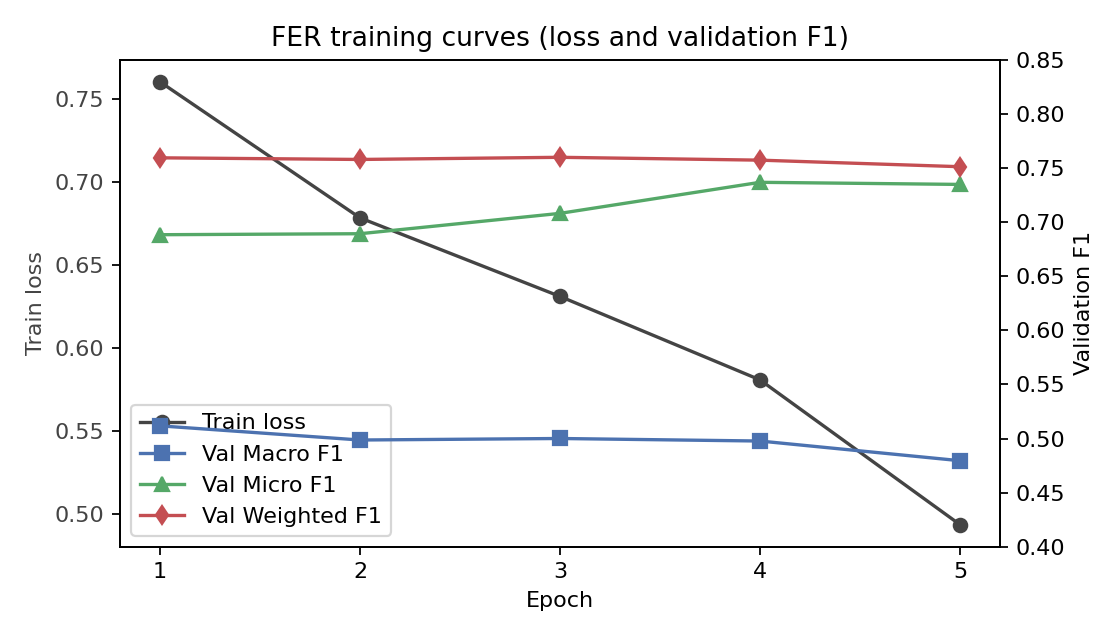
\includegraphics[width=0.85\textwidth]{Figures/fer_training_curves.png}
    \caption{Training loss and validation Macro/Micro/Weighted F1 across epochs for the chosen FER model (ResNet50~+~SE~+~two-layer BiLSTM~+~temporal attention, $24$~frames, weighted BCE with controlled oversampling, per-label tuned thresholds). The training loss decreases monotonically while the validation metrics stay inside a stable band, with the highest validation Macro F1 reached at the first epoch and used for early stopping.}
    \label{fig:fer_training_curves}
\end{figure}

The fact that the best validation Macro F1 is reached so early is, on its own, a useful diagnostic. Because the ResNet50 backbone is initialised from ImageNet \cite{he_resnet_2016} and only fine-tuned with a small learning rate of $5 \times 10^{-5}$, most of the visual representation needed for academic affect is already in place at the start of training. The remaining epochs mostly improve the ranking on the training split but stop translating into validation gains, which is exactly the regime in which an early-stopping rule based on validation Macro F1 is meant to act \cite{abedi_improving_2021,shiri_detection_2024,su_leveraging_2024}.

\subsection{Overall and Per-Label Test Performance}\label{sec:results_fer_overall}

On the official DAiSEE test set ($N_{\mathrm{test}} = 1{,}784$ clips), the chosen model reaches a Macro F1 of $0.453$, a Micro F1 of $0.724$, a Weighted F1 of $0.798$, a Samples F1 of $0.746$, and an exact-match accuracy of $0.342$. The per-label accuracies are $0.46$ for boredom, $0.95$ for engagement, $0.80$ for confusion, and $0.91$ for frustration. The per-label F1 scores are $0.36$ for boredom, $0.97$ for engagement, $0.22$ for confusion, and $0.25$ for frustration, with per-label recalls of $0.71$, $1.00$, $0.32$, and $0.34$ respectively. These numbers are summarised in Table~\ref{tab:fer_results}, while Figure~\ref{fig:fer_per_label_metrics} shows the per-label precision, recall, and F1 side by side, Figure~\ref{fig:fer_overall_metrics_bar} shows the five overall metrics in a single bar chart, and Figure~\ref{fig:fer_confusion_per_label} shows the per-label confusion matrices.

\begin{table}[H]
\centering
\caption{Test-set performance of the proposed FER model on DAiSEE.}
\label{tab:fer_results}
\begin{tabular}{lcccc}
\toprule
\textbf{Label} & \textbf{Threshold} & \textbf{Precision} & \textbf{Recall} & \textbf{F1} \\
\midrule
Boredom     & 0.30 & 0.24 & 0.71 & 0.36 \\
Engagement  & 0.10 & 0.95 & 1.00 & 0.97 \\
Confusion   & 0.60 & 0.17 & 0.32 & 0.22 \\
Frustration & 0.60 & 0.20 & 0.34 & 0.25 \\
\midrule
\textbf{Macro avg}    & --   & 0.39 & 0.59 & 0.45 \\
\textbf{Micro avg}    & --   & 0.61 & 0.88 & 0.72 \\
\textbf{Weighted avg} & --   & 0.76 & 0.88 & 0.80 \\
\textbf{Samples avg}  & --   & 0.70 & 0.91 & 0.75 \\
\textbf{Exact match}  & --   & \multicolumn{3}{c}{0.342} \\
\bottomrule
\end{tabular}
\end{table}

\begin{figure}[H]
    \centering
    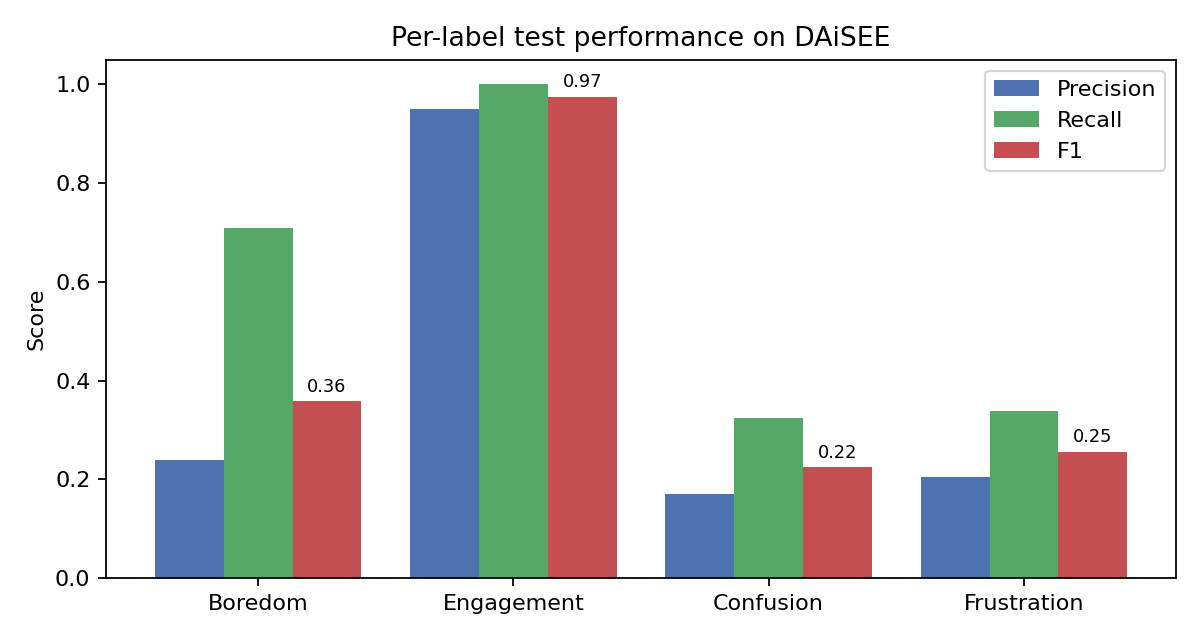
\includegraphics[width=0.92\textwidth]{Figures/fer_per_label_metrics.png}
    \caption{Per-label precision, recall, and F1 on the DAiSEE test split with the per-label thresholds reported in Table~\ref{tab:fer_results}. Engagement is detected very reliably; the rare states (boredom, confusion, frustration) trade precision for recall.}
    \label{fig:fer_per_label_metrics}
\end{figure}

\begin{figure}[H]
    \centering
    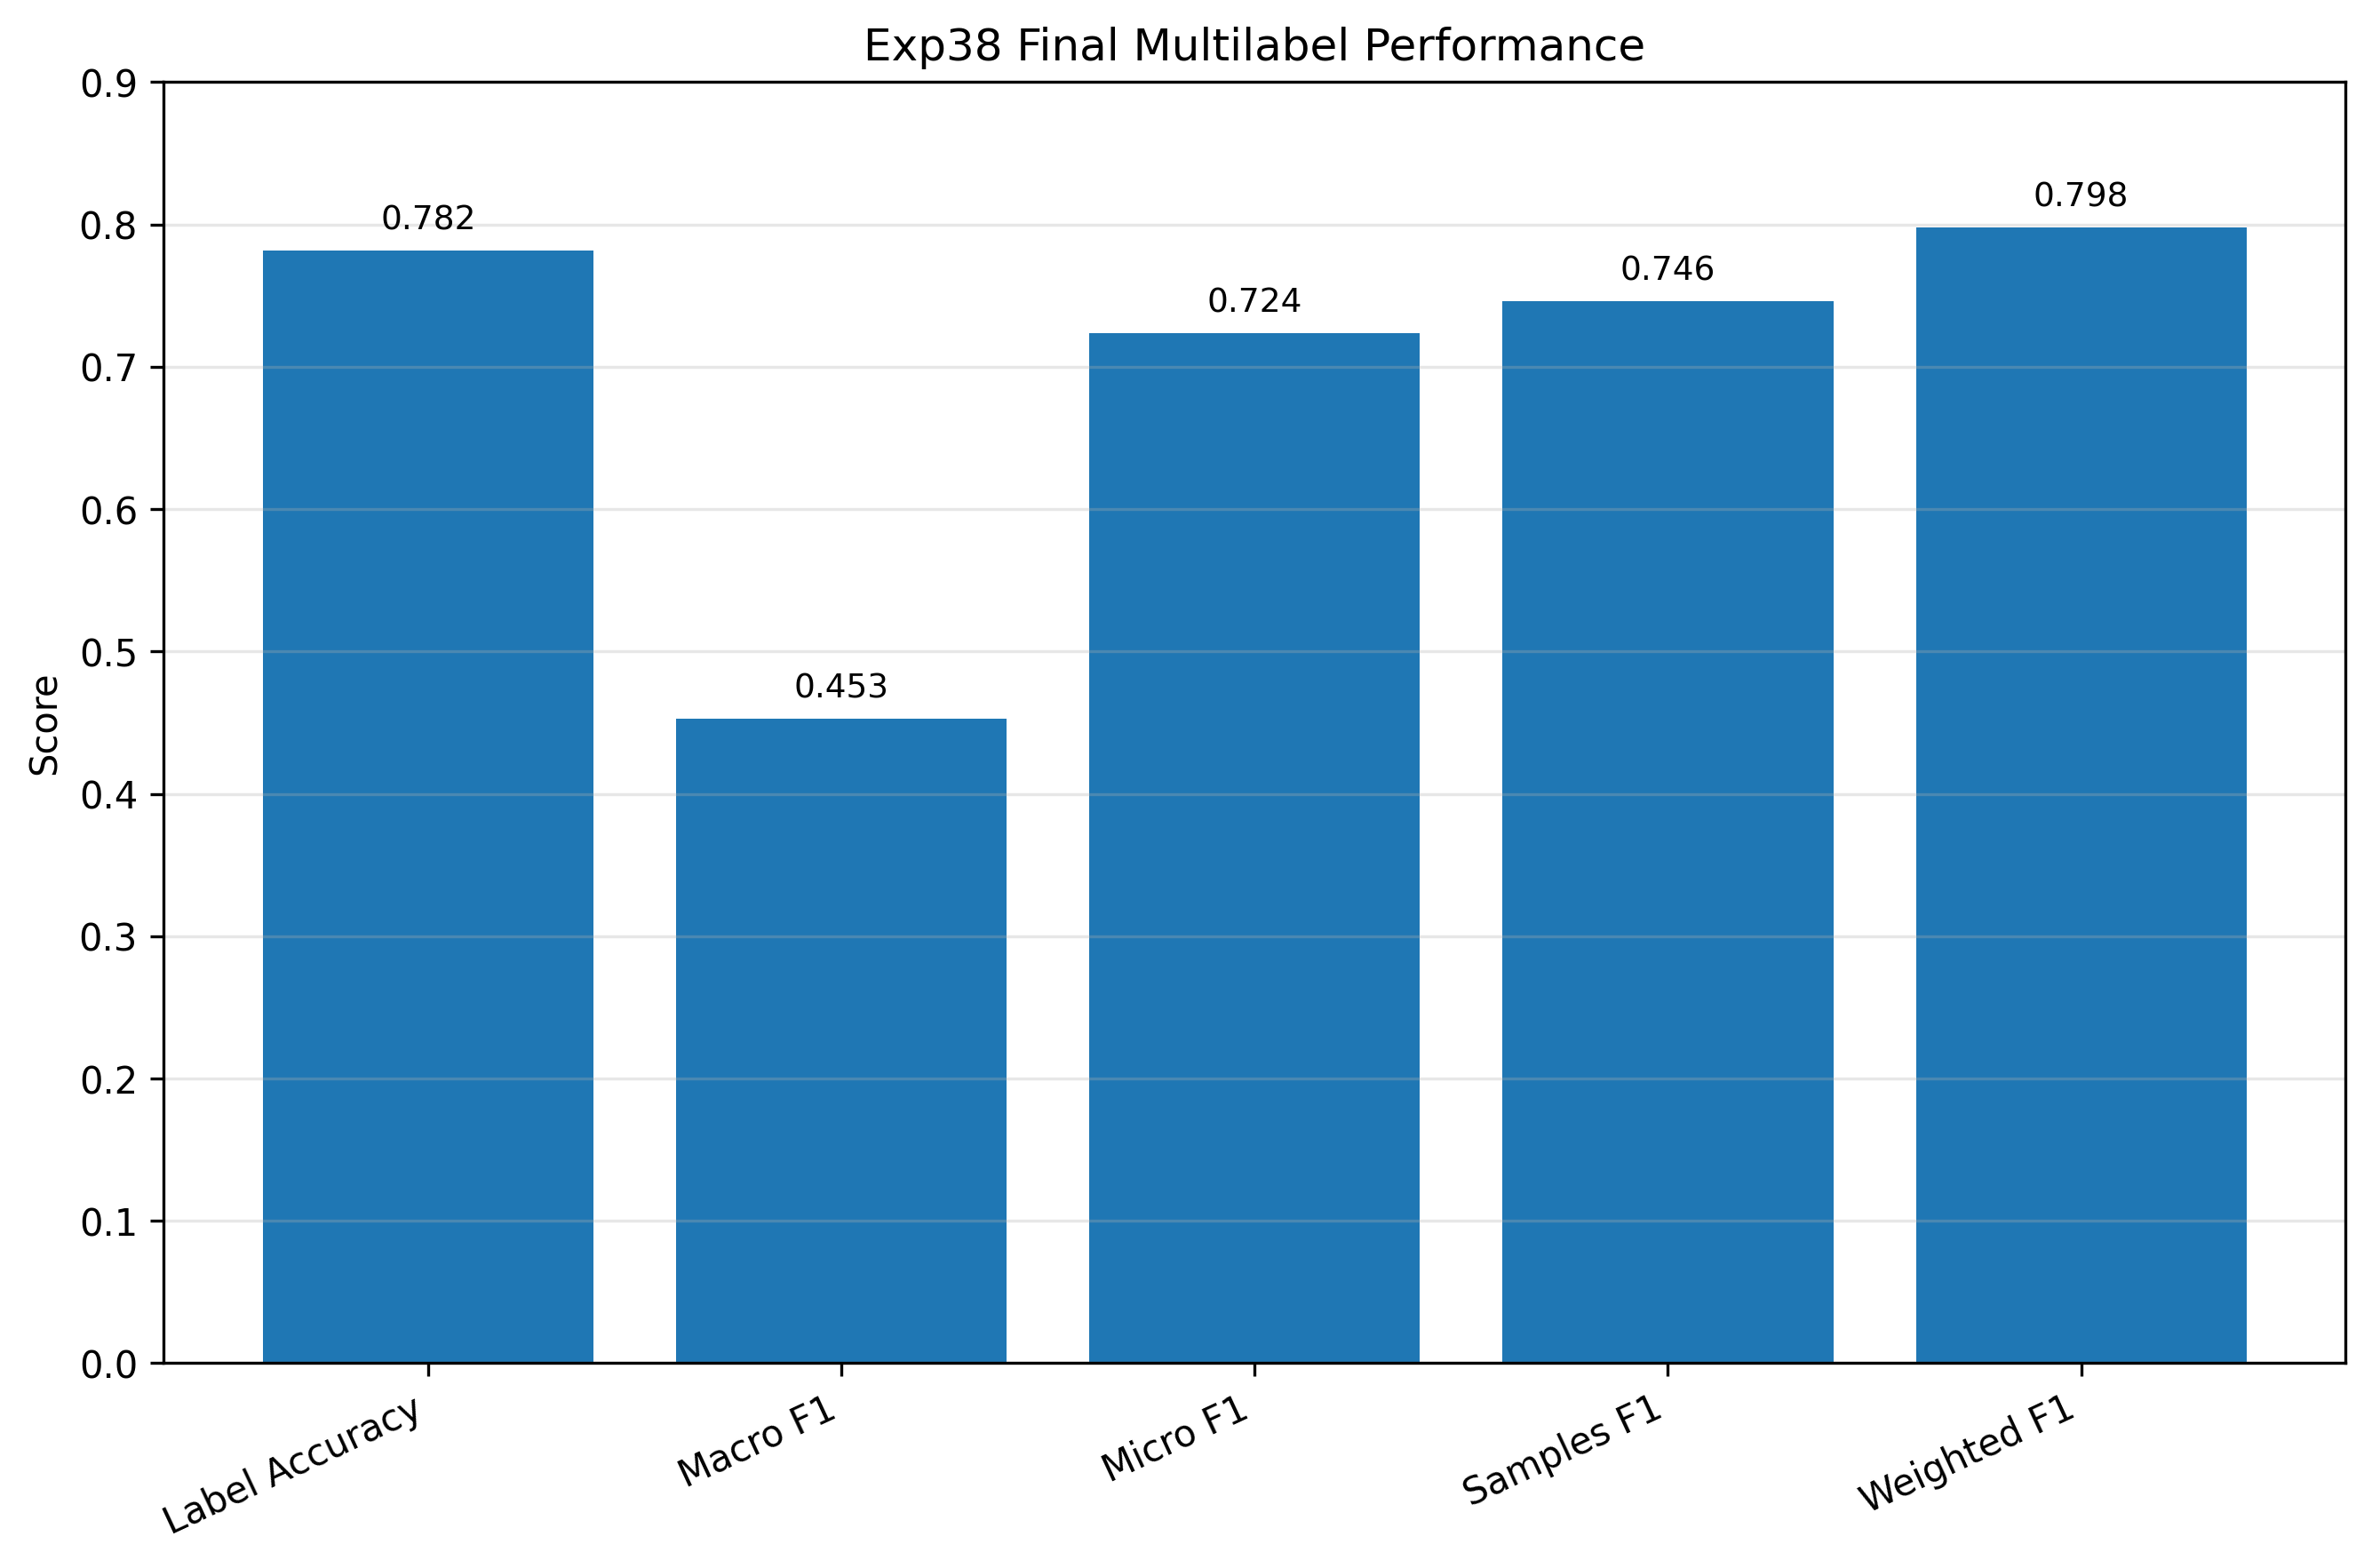
\includegraphics[width=0.78\textwidth]{Figures/fer_overall_metrics_bar.png}
    \caption{Overall test metrics of the chosen FER model on DAiSEE: per-label accuracy averaged across the four labels, Macro F1, Micro F1, Samples F1, and Weighted F1. Weighted-by-frequency metrics are noticeably higher than Macro F1, which is the expected pattern for a heavily imbalanced multilabel task in which the dominant label is very well detected.}
    \label{fig:fer_overall_metrics_bar}
\end{figure}

\begin{figure}[H]
    \centering
    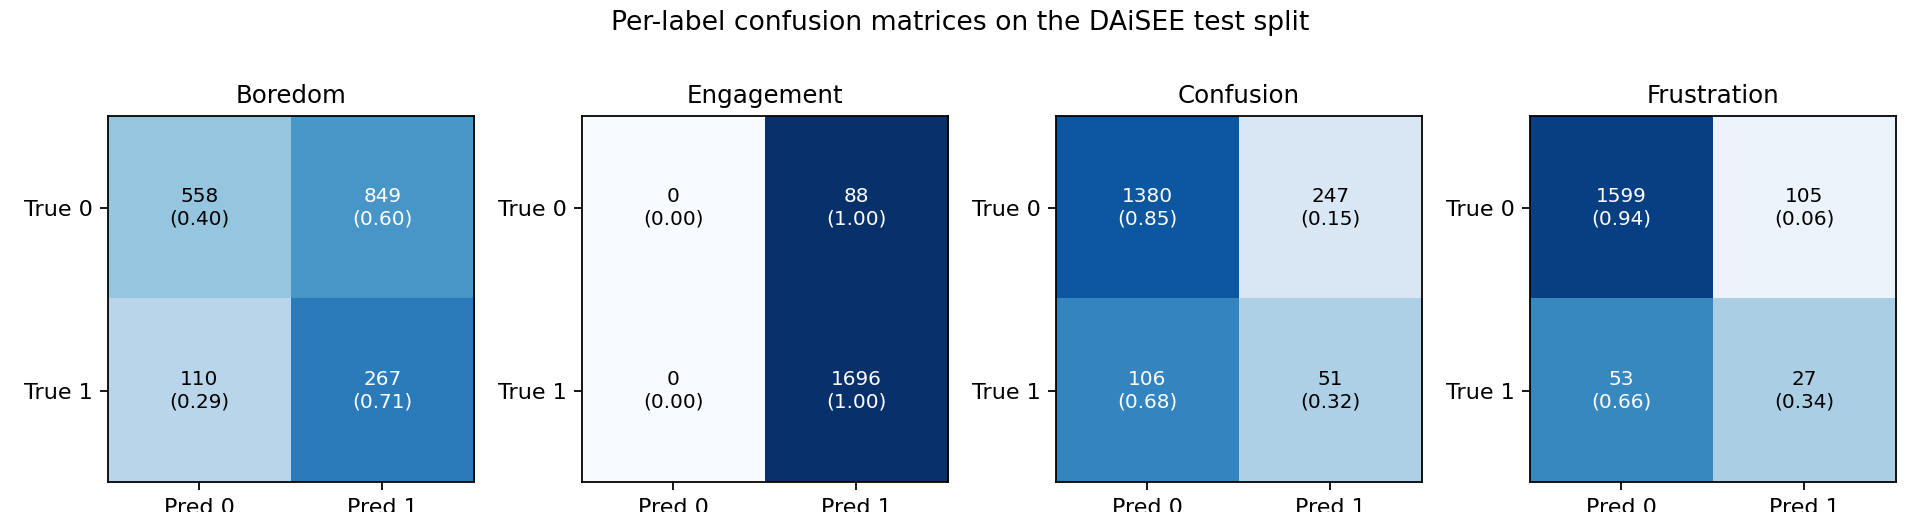
\includegraphics[width=\textwidth]{Figures/fer_confusion_per_label.png}
    \caption{Per-label confusion matrices on the DAiSEE test split. Each cell shows the absolute count and (in parentheses) the row-normalised proportion. Rows correspond to ground-truth labels and columns correspond to predicted labels for the matching emotion.}
    \label{fig:fer_confusion_per_label}
\end{figure}

The five overall metrics give complementary views of the same predictions. Weighted F1 ($0.80$) and Micro F1 ($0.72$) are high because they are dominated by the most frequent label, engagement, which the model recognises almost perfectly. Samples F1 ($0.75$) is also high because most clips contain the engagement label and predicting it correctly already lifts the per-clip F1. Macro F1 ($0.45$), however, gives equal weight to all four labels, including the rare ones, and falls noticeably below the other three because boredom, confusion, and frustration are still much harder than engagement, even with imbalance-aware training. Exact-match accuracy ($0.34$) is the strictest metric of the five: a clip is only counted as correct when all four binary labels are predicted correctly, so a single missed minority label is enough to mark the entire clip as wrong. The fact that exact match is much lower than per-label accuracy is a known property of multilabel classification under imbalance and is consistent with what is reported in recent multilabel FER works \cite{rianto_engagement_2025,fu_integrating_2025}.

The bar chart in Figure~\ref{fig:fer_per_label_metrics} also makes the precision--recall trade-off visible. The chosen thresholds were tuned on the validation split to maximise per-label F1, but because the training distribution is heavily skewed toward engagement, the rare labels still need fairly low thresholds and end up with high recall at the cost of low precision. This is a common pattern in imbalance-aware multilabel pipelines: when minority labels are sparse, the model has to choose between predicting them often (high recall, low precision) or rarely (low recall, high precision) \cite{santoni_convolutional_2023,rianto_engagement_2025}. Per-label threshold tuning, exactly because it is per-label, is what allows boredom to have a different trade-off from engagement, and confusion to have a different trade-off from frustration. Without it, a single fixed threshold of $0.5$ would either suppress almost all rare positives or flood the rare labels with false positives.

\subsection{Per-Label Analysis}\label{sec:results_fer_perlabel}

The per-label confusion matrices in Figure~\ref{fig:fer_confusion_per_label} show, for each affective label, how often the model is right or wrong, broken down by ground-truth value. The remainder of this subsection discusses each label in turn.

\paragraph{Engagement.} The model detects engagement very reliably: per-label accuracy is $0.95$, recall is $1.00$, precision is $0.95$, and F1 is $0.97$. This near-perfect recall indicates that, with the tuned threshold of $0.10$, the model essentially flags every truly engaged clip as engaged. The reason engagement dominates is structural. Engagement is by far the most frequent positive label in DAiSEE, and the controlled oversampling of Section~\ref{sec:method_preparation} keeps engagement at multiplier~$1$ while boosting rarer labels, so engagement is still the class with the strongest training signal. Engagement also corresponds to facial cues that are clearer than the other three: alert eyes, a stable head pose, a slightly forward-leaning posture, and a generally relaxed expression \cite{dmello_language_2012,asaju_adaptive_2022,asaju_affects_2021,tulsani_realtime_2025}. Recent DAiSEE engagement detectors, even when they ignore the other three labels entirely, also report engagement metrics that are well above $0.90$, which suggests that the visual cues for engagement are not particularly difficult once a strong CNN backbone is paired with a temporal model \cite{abedi_improving_2021,asaju_adaptive_2022,shiri_detection_2024,su_leveraging_2024,liu_dynamic_nodate}.

\paragraph{Boredom.} Boredom is the most informative case in the per-label results. The per-label accuracy is $0.46$, the recall is $0.71$, the precision is $0.24$, and the F1 is $0.36$. The model therefore catches most truly bored clips, but it also marks many engaged clips as bored. There are three reasons for this behaviour. First, boredom is sparse in DAiSEE relative to engagement \cite{gupta_daisee_2016,abedi_improving_2021}, so a single missed positive costs more in F1 than in accuracy. Second, the visual cues that signal boredom in a study setting are subtle: a slightly drooping eyelid, a small loss of facial tension, or a slow blink rate, none of which are as expressive as a smile or a frown \cite{dmello_language_2012,santoni_convolutional_2023}. Third, boredom and a calm, neutral form of engagement look very similar from a webcam, especially when the head pose is stable and the lighting is uniform; learners can be quietly attentive but with a low-energy face that resembles boredom. The chosen threshold of $0.30$ for boredom is the most aggressive among the three rare labels, which is what produces the high recall and low precision profile observed here, and is consistent with the pattern reported by other DAiSEE-focused works that explicitly target boredom recovery \cite{santoni_convolutional_2023,rianto_engagement_2025}.

\paragraph{Confusion.} Confusion is the hardest label in the test results. The per-label accuracy is $0.80$, but the precision is $0.17$, the recall is $0.32$, and the F1 is $0.22$. The high accuracy is misleading: confusion is itself rare, so always predicting ``not confused'' would already give an accuracy close to $0.83$. The poor F1 reflects the real difficulty. From a webcam, confusion is signalled by short and ambiguous events, such as a brief brow furrow, a small head tilt, or a momentary squint. Many of these cues only last for a few hundred milliseconds, and they overlap visually with thinking, surprise, or even mild discomfort, which DAiSEE does not separate \cite{gupta_daisee_2016,dmello_language_2012}. The temporal attention layer of the model is meant to focus on the few frames that contain the strongest cues, but when the cues themselves are subtle, even the best frames are hard to interpret correctly. Other DAiSEE studies also report that confusion is one of the labels with the weakest per-class performance, so this thesis is not unusual in that respect; what matters is that the F1 is no longer zero, which it would be under the early baselines reported in Section~\ref{sec:results_fer_arch_selection}.

\paragraph{Frustration.} Frustration is similarly hard. The per-label accuracy is $0.91$, but the precision is $0.20$, the recall is $0.34$, and the F1 is $0.25$. The pattern is the same as for confusion: rare positives, ambiguous cues, and a high accuracy that mostly reflects the dominant ``not frustrated'' class. Frustration in a study setting is even harder than in classical FER, because learners often try to suppress visible frustration in front of a webcam, which leaves only weak micro-cues such as lip pressing, jaw tension, or short exhalations \cite{dmello_language_2012,Baker2010BetterFrustratedThanBored}. The model nevertheless reaches a non-trivial F1 of $0.25$, which is again much better than the zero-recall behaviour of the early multilabel baselines.

The four cases together illustrate why Macro F1 is the right primary metric in this thesis. If the model is judged by accuracy or by Weighted F1 alone, it looks almost solved. If it is judged by Macro F1, which gives equal weight to engagement and to the three rare labels, the difficulty of the task becomes visible, and the design choices that target rare labels, such as oversampling, weighted BCE, and per-label threshold tuning, are seen as having real, but partial, effect.

\subsection{Architecture-Selection Experiments}\label{sec:results_fer_arch_selection}

The configuration evaluated above is not the first one tried. It was chosen after a long sequence of architecture-selection experiments that explored alternative backbones, alternative temporal modules, alternative attention placements, alternative imbalance-handling strategies, and alternative decision rules. To respect the consistency rule of Section~\ref{sec:results_fer_scope}, the experiments are reported in two separate tables. Table~\ref{tab:fer_arch_selection_multilabel} contains the multilabel runs and is the table used to justify the final choice. Table~\ref{tab:fer_arch_selection_singlelabel} contains the single-label runs, which were also explored as an alternative formulation but ultimately rejected because they cannot represent overlapping affect, as discussed in Section~\ref{sec:method_design_rationale}. All runs share the same DAiSEE training, validation, and test splits and the same evaluation protocol described in Section~\ref{sec:method_metrics}.

\subsubsection{Multilabel Family}\label{sec:results_fer_multilabel_family}

Table~\ref{tab:fer_arch_selection_multilabel} reports the multilabel architecture-selection runs and their final test metrics. ``Sampling'' indicates the data-level imbalance strategy (\textsc{none} for shuffled training, \textsc{ws} for the weighted random sampler, \textsc{os} for the controlled-oversampling CSV used by the final model). ``Loss'' indicates the optimisation-level imbalance strategy (\textsc{bce} for plain binary cross-entropy, \textsc{wbce} for weighted binary cross-entropy with a positive-class weight, \textsc{focal} for focal binary cross-entropy). ``Thr.'' indicates the decision rule (\textsc{0.5} for the fixed default, \textsc{tuned} for per-label thresholds tuned on the validation split as in Section~\ref{sec:method_thresholds}). The chosen final configuration (Exp~38) is shown in bold.

\begin{table}[H]
\centering
\small
\caption{Multilabel architecture-selection experiments on the DAiSEE test split. All runs share the same DAiSEE splits and the same evaluation protocol of Section~\ref{sec:method_metrics}. The chosen final configuration (Exp~38) is shown in bold.}
\label{tab:fer_arch_selection_multilabel}
\begin{tabular}{lp{4.4cm}cccc}
\toprule
\textbf{ID} & \textbf{Architecture} & \textbf{Sampling/Loss} & \textbf{Thr.} & \textbf{Frames} & \textbf{Macro F1} \\
\midrule
Exp 1  & ResNet50 + BiLSTM                                         & \textsc{none}/\textsc{bce}    & 0.5     & 16 & 0.251 \\
Exp 2  & ResNet50 + BiLSTM                                         & \textsc{none}/\textsc{wbce}   & 0.5     & 16 & 0.356 \\
Exp 3  & ResNet50 + BiLSTM                                         & \textsc{none}/\textsc{wbce}   & 0.3     & 16 & 0.392 \\
Exp 4  & ResNet50 + BiLSTM (5~epochs)                              & \textsc{none}/\textsc{wbce}   & 0.5     & 16 & 0.408 \\
Exp 5  & ResNet50 + BiLSTM ($\mathrm{lr}=5\!\times\!10^{-5}$)      & \textsc{none}/\textsc{wbce}   & 0.5     & 16 & 0.405 \\
Exp 6  & ResNet50 + BiLSTM (naive sampler+\textsc{wbce})           & \textsc{ws}/\textsc{wbce}     & 0.5     & 16 & 0.153 \\
Exp 8  & ResNet50 + BiLSTM (last frame)                            & \textsc{none}/\textsc{wbce}   & 0.5     & 16 & 0.303 \\
Exp 9  & ResNet50 + BiLSTM                                         & \textsc{none}/\textsc{wbce}   & 0.5     & 16 & 0.155 \\
Exp 10 & EfficientNetV2-S + BiLSTM                                 & \textsc{none}/\textsc{wbce}   & 0.5     & 16 & 0.379 \\
Exp 11 & EfficientNetV2-S + Transformer                            & \textsc{none}/\textsc{wbce}   & 0.5     & 8  & 0.319 \\
Exp 12 & ShuffleNetV2 + SE + BiLSTM                                & \textsc{none}/\textsc{wbce}   & 0.5     & 16 & 0.404 \\
Exp 13 & Xception + BiLSTM                                         & \textsc{none}/\textsc{bce}    & 0.5     & 16 & 0.246 \\
Exp 14 & SE-ResNet50 + BiLSTM + temp.\ attn.                       & \textsc{none}/\textsc{bce}    & 0.5     & 16 & 0.280 \\
Exp 15 & ResNet18 + Transformer                                    & \textsc{none}/\textsc{bce}    & 0.5     & 16 & 0.305 \\
Exp 16 & ShuffleNetV2 + SE + 2-BiLSTM                              & \textsc{ws}/\textsc{wbce}     & tuned   & 24 & 0.445 \\
Exp 17 & ShuffleNetV2 + SE + 2-BiLSTM + temp.\ attn.               & \textsc{ws}/\textsc{wbce}     & tuned   & 24 & 0.444 \\
Exp 18 & EfficientNetV2-S + 2-BiLSTM + temp.\ attn.                & \textsc{none}/\textsc{wbce}   & tuned   & 24 & 0.336 \\
Exp 19 & 3D DenseNet + 3D self-attn.                               & \textsc{none}/\textsc{focal}  & 0.5     & 16 & 0.379 \\
Exp 34 & ResNet50 + BiLSTM + temp.\ attn.                          & \textsc{os}/\textsc{bce}      & 0.5     & 16 & 0.383 \\
\textbf{Exp 38 (final)} & \textbf{ResNet50 + SE + 2-BiLSTM + temp.\ attn.} & \textbf{\textsc{os}/\textsc{wbce}} & \textbf{tuned} & \textbf{24} & \textbf{0.453} \\
\bottomrule
\end{tabular}
\end{table}

The structure of Table~\ref{tab:fer_arch_selection_multilabel} carries the main empirical narrative of the chapter, and is matched by the bar chart in Figure~\ref{fig:fer_macro_f1_comparison}, which contrasts the strongest single-label, multilabel and traditional baselines side-by-side, and by the weighted-F1 bar chart in Figure~\ref{fig:fer_weighted_f1_comparison}. The conclusions visible from the table can be grouped into five lessons.

\paragraph{Lesson 1: Imbalance handling is the single most important axis.} The plain BCE baselines without any imbalance handling, Exp~1 with ResNet50~+~BiLSTM and Exp~13 with Xception~+~BiLSTM, only reach Macro F1 of $0.251$ and $0.246$ respectively. Adding a positive-class weight to the loss (\textsc{wbce}) lifts the same backbone~+~temporal model from $0.251$ in Exp~1 to $0.356$ in Exp~2, and to $0.408$ once the run is given five epochs in Exp~4. This is consistent with what other DAiSEE works report: without imbalance-aware training, multilabel models on DAiSEE collapse to engagement and produce nearly zero F1 on the rare labels \cite{abedi_improving_2021,santoni_convolutional_2023,rianto_engagement_2025}.

\paragraph{Lesson 2: Imbalance handling can also be overdone.} Exp~6 combines a naive weighted random sampler with the same weighted BCE used in Exp~5 and obtains a Macro F1 of only $0.153$, with Engagement F1 collapsing to $0.000$. This is the worst multilabel result in the entire table, even though it uses the most aggressive imbalance correction. The reason is that the sampler and the loss correct for the same imbalance twice, which over-emphasises minority clips so strongly that the model loses the dominant class. The lesson is that data-level and loss-level corrections must be jointly calibrated, not stacked blindly. The chosen final configuration in Exp~38 instead uses a controlled, fixed-multiplier oversampling (engagement~$\times 1$, boredom~$\times 2$, confusion~$\times 3$, frustration~$\times 4$), which is much milder than the inverse-frequency sampler of Exp~6 and combines well with the clipped per-label \texttt{pos\_weight}.

\paragraph{Lesson 3: A heavier or more modern backbone is not automatically better.} EfficientNetV2-S in Exp~10 gives Macro F1 $0.379$, slightly below the ShuffleNetV2 ShuffleNetV2~+~SE backbone of Exp~12 ($0.404$) on the same temporal head, despite EfficientNetV2-S being a much heavier model. Xception in Exp~13 gives only $0.246$, even though Xception is a strong classical FER backbone in non-educational benchmarks. SE-ResNet50 in Exp~14, which adds an integrated SE block inside ResNet50 plus a temporal attention layer, gives $0.280$, well below ResNet50~+~BiLSTM~+~\textsc{wbce} (Exp~4, $0.408$). The general pattern is that backbone strength alone does not solve DAiSEE, which is in line with what recent surveys observe: educational FER datasets are too small and too imbalanced for backbone scaling to behave the way it does on ImageNet \cite{lek_academic_2023,vistorte_integrating_2024,florestiyanto_emotion_2024}.

\paragraph{Lesson 4: Two-layer BiLSTM with temporal attention beats one-layer BiLSTM with a last-frame readout.} Among the runs that share weighted BCE and a similar imbalance setup, the temporal-attention variants (Exp~16, Exp~17, Exp~38) consistently sit at the top of the table, while the last-frame readouts (Exp~8) sit near the middle. Exp~17, which adds a temporal attention layer on top of the same ShuffleNetV2~+~SE~+~2-BiLSTM as Exp~16, reaches Macro F1 $0.444$ versus $0.445$ for Exp~16; the two are essentially tied. Exp~38, which keeps the same two-layer BiLSTM~+~temporal attention but switches the backbone to ResNet50, lifts the Macro F1 further to $0.453$. This is the empirical evidence behind the design choice in Section~\ref{sec:method_temporal_attention}: pooling time steps with attention, instead of taking the last hidden state, lets the model focus on the few frames that actually contain affect-relevant cues, which is consistent with the same conclusion in other DAiSEE pipelines that compare temporal pooling strategies \cite{mehta_three-dimensional_2022,su_leveraging_2024,liu_dynamic_nodate}.

\paragraph{Lesson 5: Per-label threshold tuning is decisive.} Exp~3 takes the same model as Exp~2 but moves the decision threshold from $0.5$ to $0.3$, lifting Macro F1 from $0.356$ to $0.392$. The price is that overall accuracy drops sharply, because lowering the threshold floods minority labels with false positives. A single fixed threshold therefore cannot be optimal for all four labels at once. Per-label thresholds, tuned on the validation split as described in Section~\ref{sec:method_thresholds}, fix this: Exp~16, Exp~17 and Exp~38, which use per-label tuned thresholds, are the three highest-scoring multilabel runs, with Macro F1 between $0.444$ and $0.453$.

The chosen Exp~38 sits at the intersection of these five lessons. It uses a strong but conventional ResNet50 backbone (Lesson~3), an SE block plus a two-layer BiLSTM with temporal attention as the temporal module (Lesson~4), a jointly calibrated combination of controlled oversampling and weighted BCE (Lessons~1--2), and per-label thresholds tuned on the validation set (Lesson~5). The result, a test Macro F1 of $0.453$, is the highest in Table~\ref{tab:fer_arch_selection_multilabel}.

\begin{figure}[H]
    \centering
    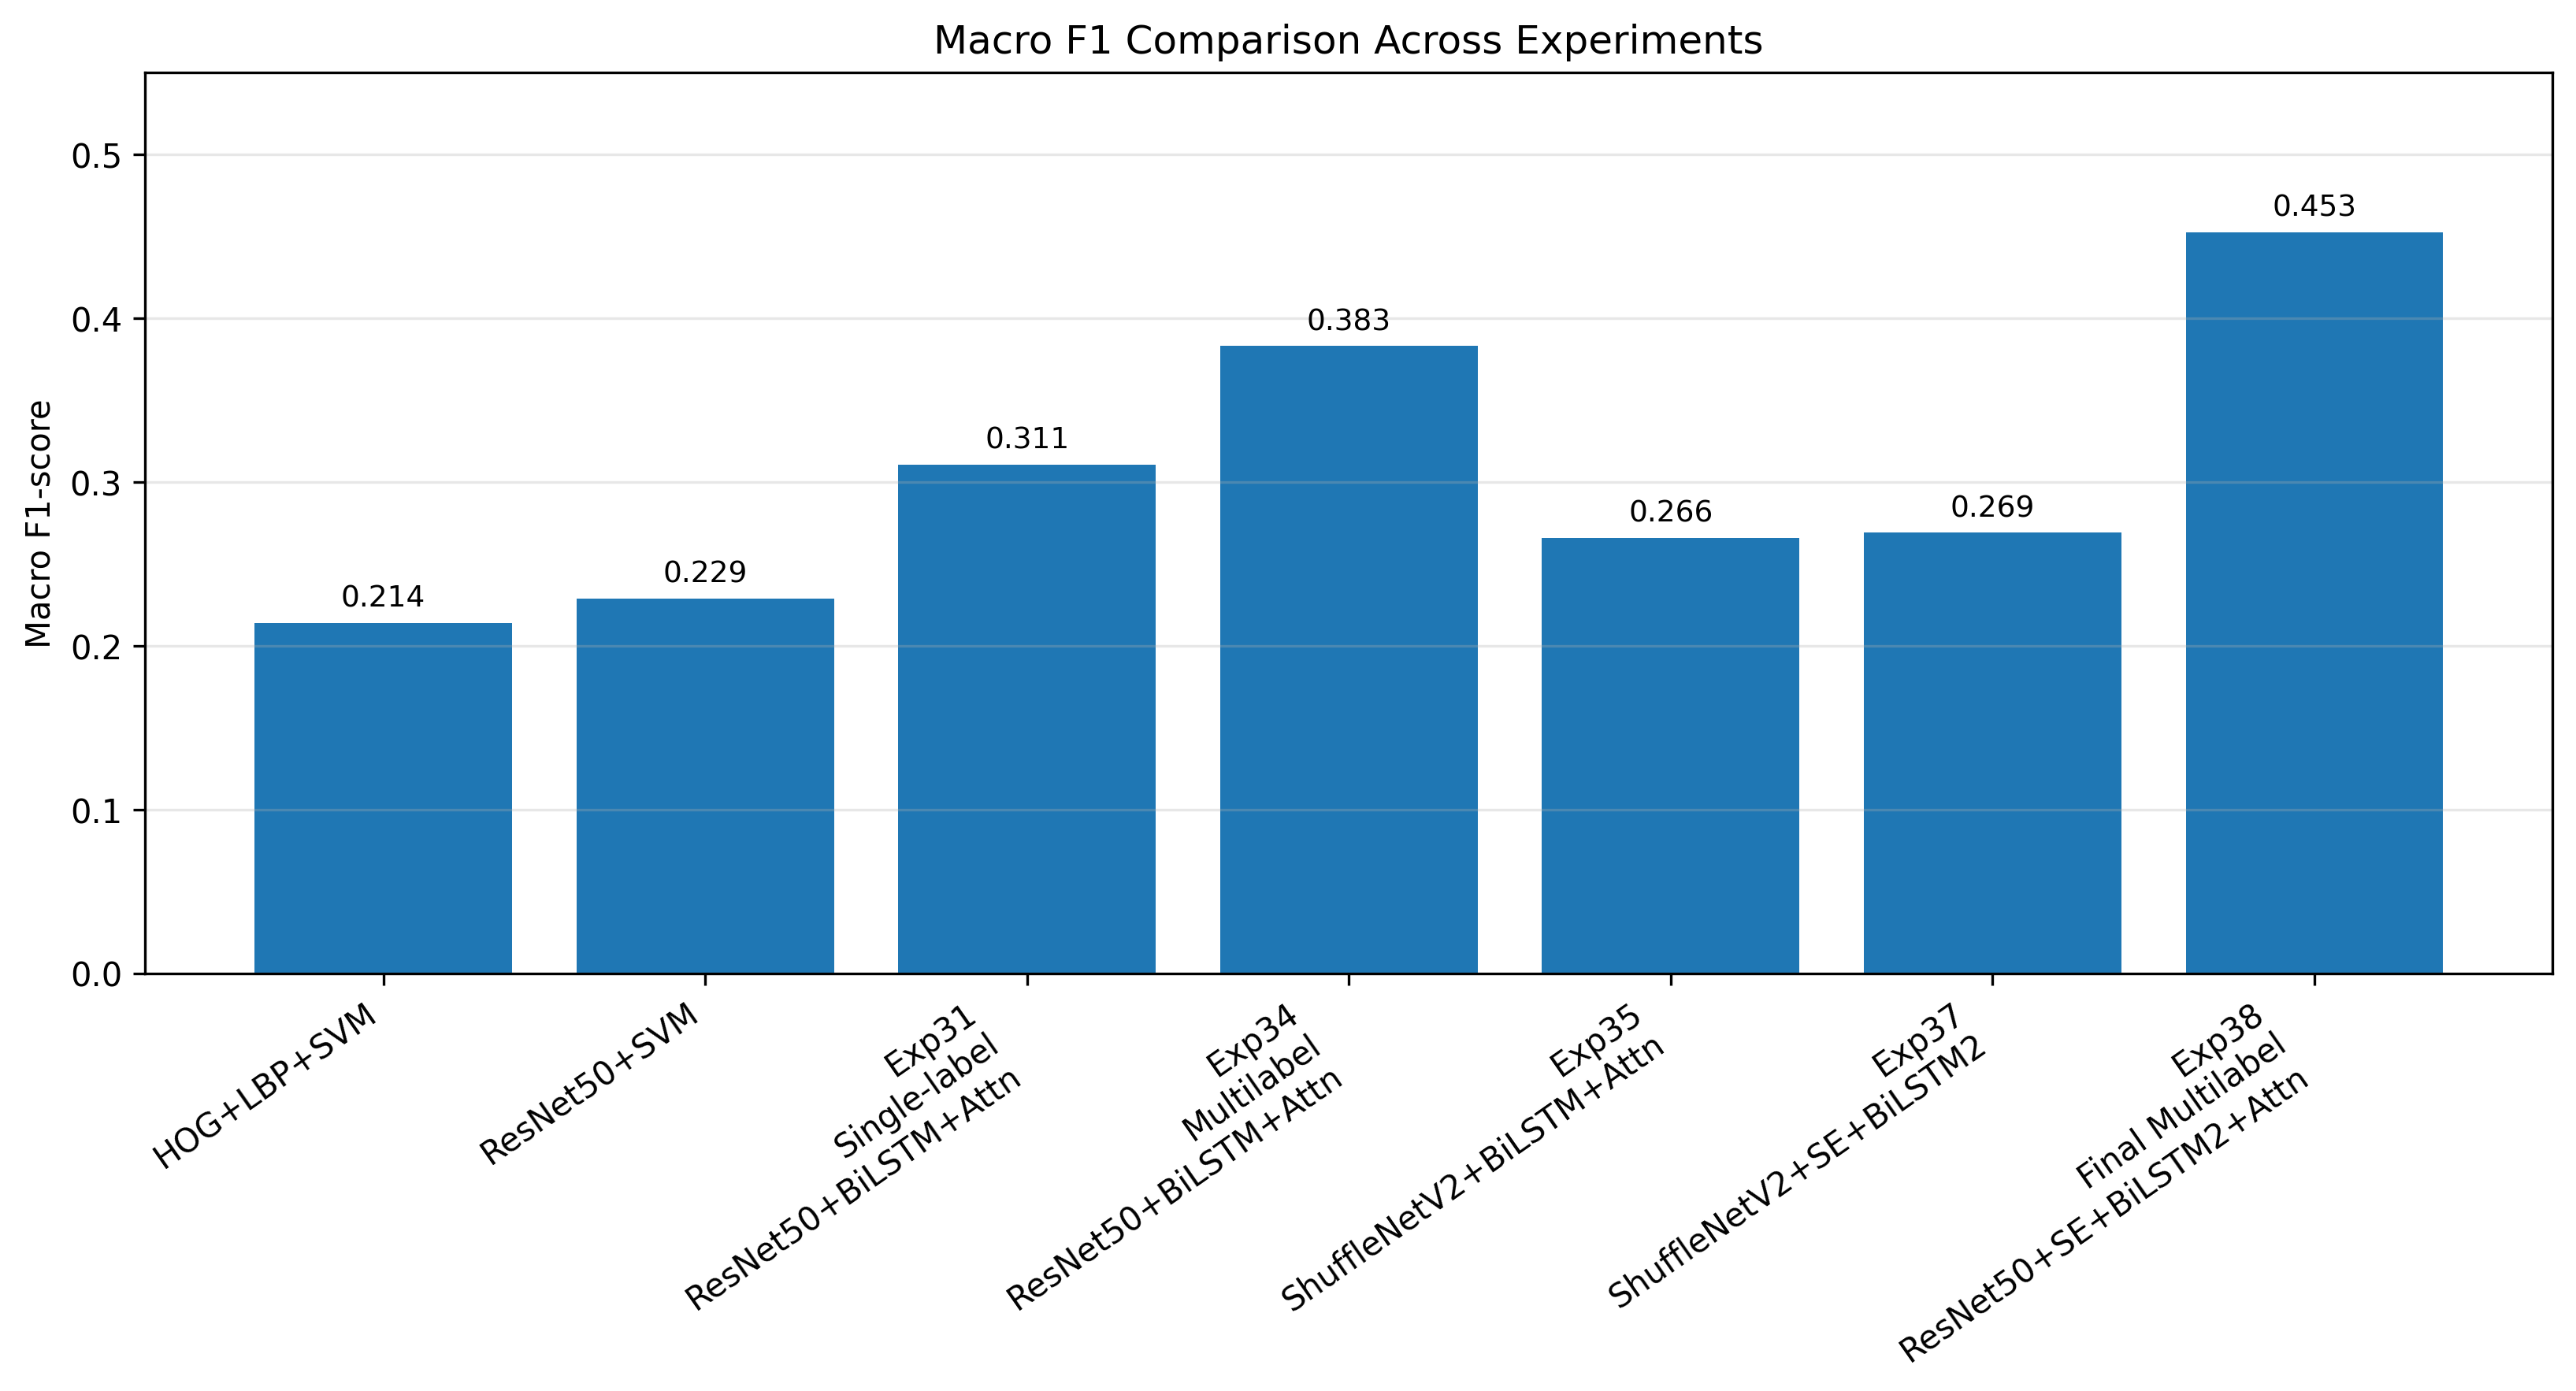
\includegraphics[width=0.92\textwidth]{Figures/fer_macro_f1_comparison.png}
    \caption{Macro F1 across the strongest multilabel and single-label experiments and the two traditional baselines (HOG~+~LBP~+~SVM and ResNet50 features~+~SVM). The chosen final model, Exp~38, dominates all other runs on Macro F1, and the multilabel runs on the right of the chart all sit above their single-label counterparts trained under matched protocols.}
    \label{fig:fer_macro_f1_comparison}
\end{figure}

\subsubsection{Single-Label Family}\label{sec:results_fer_singlelabel_family}

Table~\ref{tab:fer_arch_selection_singlelabel} reports the single-label family experiments. These runs use the same DAiSEE training, validation and test splits, but they predict only the single dominant emotion of the clip with a softmax head and a cross-entropy or focal cross-entropy loss. Because the multilabel-style metrics (Micro F1, Samples F1, Weighted F1) are not defined in exactly the same way for single-label classification, only multiclass Macro F1, Weighted F1, and accuracy are reported here. The strongest single-label run is shown in bold, but it is \emph{not} the model used in the rest of the thesis: as discussed in Section~\ref{sec:results_fer_scope} and motivated in Section~\ref{sec:method_design_rationale}, the multilabel formulation is preferred because it can represent overlapping affect, which the single-label formulation cannot.

\begin{table}[H]
\centering
\small
\caption{Single-label architecture-selection experiments on the DAiSEE test split. ``Macro F1'' is the multiclass macro-averaged F1; ``Weighted F1'' is multiclass weighted F1; ``Acc.'' is multiclass top-1 accuracy. The strongest single-label run (Exp~31) is shown in bold; it is \emph{not} the model used in the rest of the thesis, because the single-label formulation cannot represent overlapping affect.}
\label{tab:fer_arch_selection_singlelabel}
\begin{tabular}{lp{4.4cm}lcccc}
\toprule
\textbf{ID} & \textbf{Architecture} & \textbf{Loss/Sampling} & \textbf{Frames} & \textbf{Macro F1} & \textbf{Weighted F1} & \textbf{Acc.} \\
\midrule
Exp 22 & ResNet50 + BiLSTM                                         & CE/\textsc{ws}            & 16 & 0.282 & 0.648 & 0.656 \\
Exp 23 & ResNet50 + BiLSTM + temp.\ attn.                          & focal CE/\textsc{ws}      & 16 & 0.310 & 0.657 & 0.665 \\
Exp 24 & ShuffleNetV2 + BiLSTM (last frame)                        & CE/balanced CSV           & 16 & 0.232 & 0.549 & 0.525 \\
Exp 25 & ResNet50 + CBAM + TCN                                     & CE/\textsc{ws}            & 16 & 0.275 & 0.613 & 0.608 \\
Exp 26 & FaceNet (frozen) + BiLSTM                                 & CE/\textsc{ws}            & 16 & 0.191 & 0.334 & 0.269 \\
Exp 27 & 3D DenseNet + 3D self-attn.                               & CE/\textsc{ws}            & 16 & 0.171 & 0.273 & 0.235 \\
Exp 28 & ShuffleNetV2 + BiLSTM + multihead attn.                   & focal CE/\textsc{ws}      & 16 & 0.264 & 0.566 & 0.516 \\
Exp 30 & ResNet50 + CBAM + 3D CNN (AGTO)                           & focal CE/\textsc{ws}      & 16 & 0.267 & 0.510 & 0.448 \\
\textbf{Exp 31} & \textbf{ResNet50 + BiLSTM + temp.\ attn.}        & \textbf{focal CE/balanced CSV} & \textbf{16} & \textbf{0.311} & \textbf{0.666} & \textbf{0.702} \\
Exp 35 & ShuffleNetV2 + BiLSTM + temp.\ attn.                      & focal CE/balanced CSV     & 16 & 0.266 & 0.621 & 0.631 \\
Exp 36 & ResNet50 + 2-BiLSTM + temp.\ attn.                        & focal CE/balanced CSV     & 24 & 0.271 & 0.602 & 0.581 \\
Exp 37 & ShuffleNetV2 + SE + 2-BiLSTM + temp.\ attn.               & focal CE/balanced CSV     & 24 & 0.269 & 0.635 & 0.651 \\
\bottomrule
\end{tabular}
\end{table}

The single-label family produces a useful negative result. The strongest single-label run, Exp~31 (ResNet50~+~BiLSTM~+~temporal attention with focal cross-entropy on a balanced training CSV), reaches a multiclass top-1 accuracy of $0.702$ and a Macro F1 of $0.311$. Despite the high accuracy, its per-label F1 scores remain very uneven: $0.83$ for engagement and only $0.13$, $0.16$, and $0.12$ for boredom, confusion, and frustration respectively. Other single-label runs reproduce the same pattern: they look acceptable on accuracy because most clips have ``engagement'' as their dominant label, but they collapse to engagement-only predictions on the rare labels. Even more aggressive backbones, such as InceptionResnetV1 pretrained on VGGFace2 in Exp~26 or 3D DenseNet with self-attention in Exp~27, do not fix this; in fact, they make it worse, because their higher capacity overfits the dominant class even faster.

A direct comparison between the best single-label run (Exp~31, multiclass Macro F1 $0.311$) and the chosen multilabel run (Exp~38, multilabel Macro F1 $0.453$) is shown in Figure~\ref{fig:fer_macro_f1_comparison}. The two numbers should not be read as a head-to-head improvement, because they correspond to different problems with different denominators: Exp~31 only has to pick one of four classes per clip, while Exp~38 has to commit to four binary decisions per clip. What can be claimed is the qualitative observation that, under matched training protocols and the same DAiSEE splits, the multilabel formulation does not simply trade off engagement detection for minority detection: it produces engagement F1 of $0.97$ \emph{and} non-zero F1 on all three rare labels, while every single-label run that reaches high accuracy still has at least one rare label very close to zero F1. This is the empirical counterpart of the conceptual argument in Section~\ref{sec:method_design_rationale}: academic affect overlaps in time, and forcing the model to choose only one emotion per clip throws away signal that the multilabel head can exploit.

\subsubsection{Decision-Rule Ablation: Fixed versus Per-Label Thresholds}\label{sec:results_fer_threshold_ablation}

The effect of decision-rule choice can also be read directly from Table~\ref{tab:fer_arch_selection_multilabel}. The runs with a fixed threshold of $0.5$ never exceed Macro F1 of $0.408$ (Exp~4, ResNet50~+~BiLSTM trained for five epochs with weighted BCE) and typically sit between $0.25$ and $0.40$. The runs with per-label tuned thresholds, Exp~16, Exp~17 and Exp~38, are the three highest entries in the table. Switching from a fixed $0.5$ to per-label tuned thresholds therefore lifts the chosen architecture by roughly four to five Macro F1 points, even when the underlying network is identical. This single decision rule, exposed by Exp~3 already in a one-shot threshold-of-$0.3$ ablation, turned out to be one of the most cost-effective interventions of the entire FER pipeline, because it does not require any retraining and it is computed once per validation pass.

\subsubsection{Backbone Comparison Cross-Family}\label{sec:results_fer_backbone_cross}

Across both families, the same backbones can be compared on the same temporal head. ResNet50~+~BiLSTM is used in both Exp~22 (single-label, multiclass Macro F1 $0.282$) and Exp~4 (multilabel, multilabel Macro F1 $0.408$). ShuffleNetV2~+~BiLSTM is used in both Exp~24 (single-label, $0.232$) and Exp~12 (multilabel, $0.404$). EfficientNetV2-S~+~BiLSTM is only used in the multilabel family, in Exp~10 (multilabel Macro F1 $0.379$). FaceNet (frozen) is only used in the single-label family, in Exp~26 (multiclass Macro F1 $0.191$), and is the weakest backbone in either family. Even with the formulation-mismatch caveat, the trend across both tables agrees with what most recent DAiSEE pipelines also report: ResNet50 and ShuffleNetV2 are sweet-spot backbones for educational FER, in the sense that they pair well with temporal models of moderate size and do not over-fit on a dataset that contains only $5{,}358$ training clips \cite{abedi_improving_2021,asaju_adaptive_2022,santoni_convolutional_2023,shiri_detection_2024,tulsani_realtime_2025,aly_revolutionizing_2025}.

\subsection{Comparison with Traditional and Frame-Level Baselines}\label{sec:results_fer_traditional}

Two traditional baselines were also trained on DAiSEE to provide context for the deep multilabel pipeline. The first uses HOG and LBP descriptors per frame, averaged into a single video-level feature vector, and classified with an RBF Support Vector Machine using class-balanced weights, on $8$-frame clips at $128 \times 128$ resolution. The second uses ResNet50 ImageNet features per frame, averaged into a single video-level feature vector, and classified with the same SVM family on $16$-frame clips at $224 \times 224$. Both are single-label classifiers and use no temporal model beyond average pooling. Their test results are summarised in Table~\ref{tab:fer_traditional}, and the accuracy comparison against the strongest single-label deep models is shown in Figure~\ref{fig:fer_accuracy_comparison}.

\begin{table}[H]
\centering
\footnotesize
\caption{Traditional and frame-level baselines on the DAiSEE test split. Both baselines are single-label classifiers and use no temporal model beyond per-clip average pooling. The chosen multilabel deep model is added in the last row for reference; its Macro F1 is multilabel and is not directly comparable to the multiclass Macro F1 of the SVM rows. ``Bor.'', ``Eng.'', ``Con.'', ``Fru.'' are the per-label F1 scores.}
\label{tab:fer_traditional}
\setlength{\tabcolsep}{4pt}
\begin{tabular}{lccccccc}
\toprule
\textbf{Model} & \textbf{Macro F1} & \textbf{Weighted F1} & \textbf{Acc.} & \textbf{Bor.} & \textbf{Eng.} & \textbf{Con.} & \textbf{Fru.} \\
\midrule
HOG~+~LBP~+~SVM (single-label)             & 0.214 & 0.651 & 0.750 & 0.00 & 0.86 & 0.00 & 0.00 \\
ResNet50 features~+~SVM (single-label)     & 0.229 & 0.658 & 0.759 & 0.00 & 0.86 & 0.00 & 0.05 \\
\midrule
Exp~38 (multilabel, final)                 & 0.453$^{\dagger}$ & 0.798$^{\dagger}$ & 0.342$^{\ddagger}$ & 0.36 & 0.97 & 0.22 & 0.25 \\
\bottomrule
\end{tabular}\\[0.4em]
\raggedright
\footnotesize $^{\dagger}$Multilabel Macro F1 / Weighted F1; not directly comparable to the multiclass Macro F1 of the SVM rows. $^{\ddagger}$Multilabel exact-match accuracy (all four labels correct).
\end{table}

\begin{figure}[H]
    \centering
    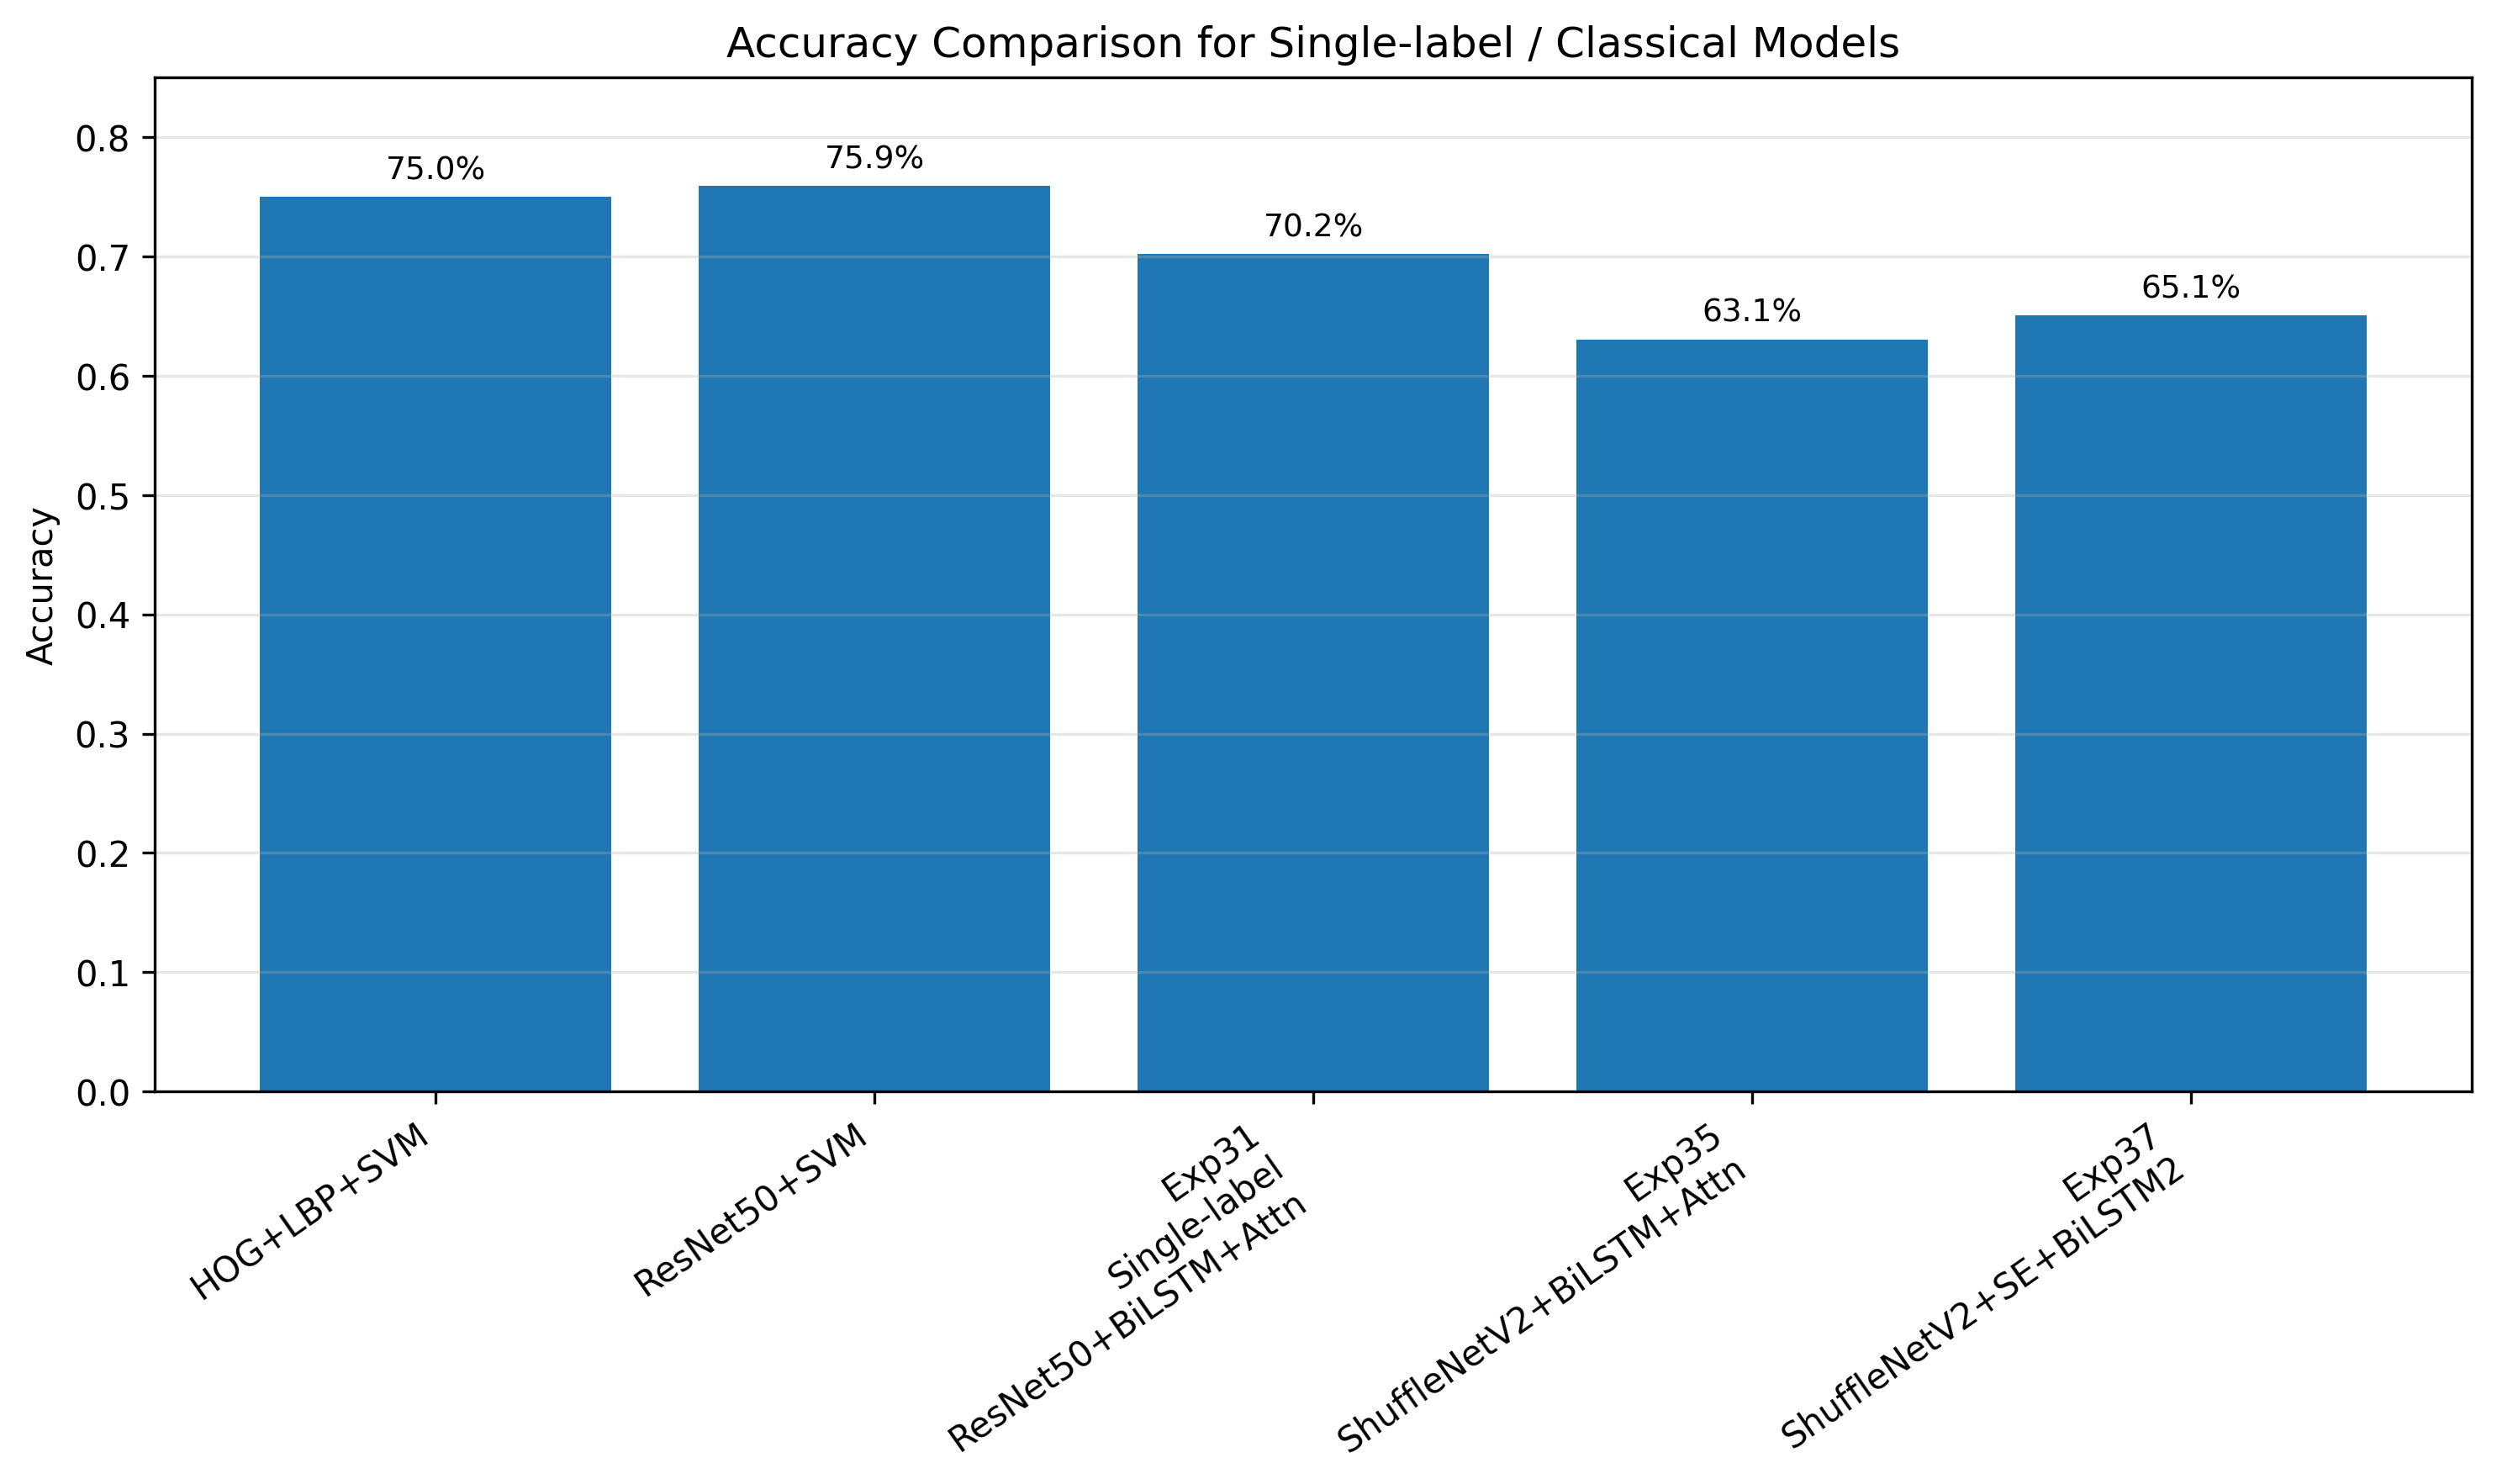
\includegraphics[width=0.92\textwidth]{Figures/fer_accuracy_comparison.png}
    \caption{Top-1 / per-label accuracy on the DAiSEE test split for the two traditional single-label baselines (HOG~+~LBP~+~SVM, ResNet50 features~+~SVM) and the strongest single-label deep models. The traditional baselines achieve high overall accuracy by collapsing to engagement, but their per-label F1 on the rare labels is essentially zero (Table~\ref{tab:fer_traditional}).}
    \label{fig:fer_accuracy_comparison}
\end{figure}

The two SVM baselines reach top-1 accuracy of $0.750$ and $0.759$, which is high. However, both models predict almost only ``engagement'': their per-label F1 is $0.00$ on boredom, $0.00$ on confusion, and $0.00$ or $0.05$ on frustration, against $0.86$ on engagement. They are therefore degenerate solutions that maximise accuracy by ignoring the minority labels, exactly as warned by Section~\ref{sec:method_metrics}. The chosen deep multilabel model, in contrast, reaches non-zero F1 on every label, and its multilabel Macro F1 of $0.453$ is roughly twice the multiclass Macro F1 of either SVM baseline, even though the two metrics are not directly comparable. The traditional baselines therefore confirm that high accuracy on DAiSEE is not, on its own, evidence of a useful FER model: a model that always predicts engagement is already at $\approx 0.75$ accuracy.

\begin{figure}[H]
    \centering
    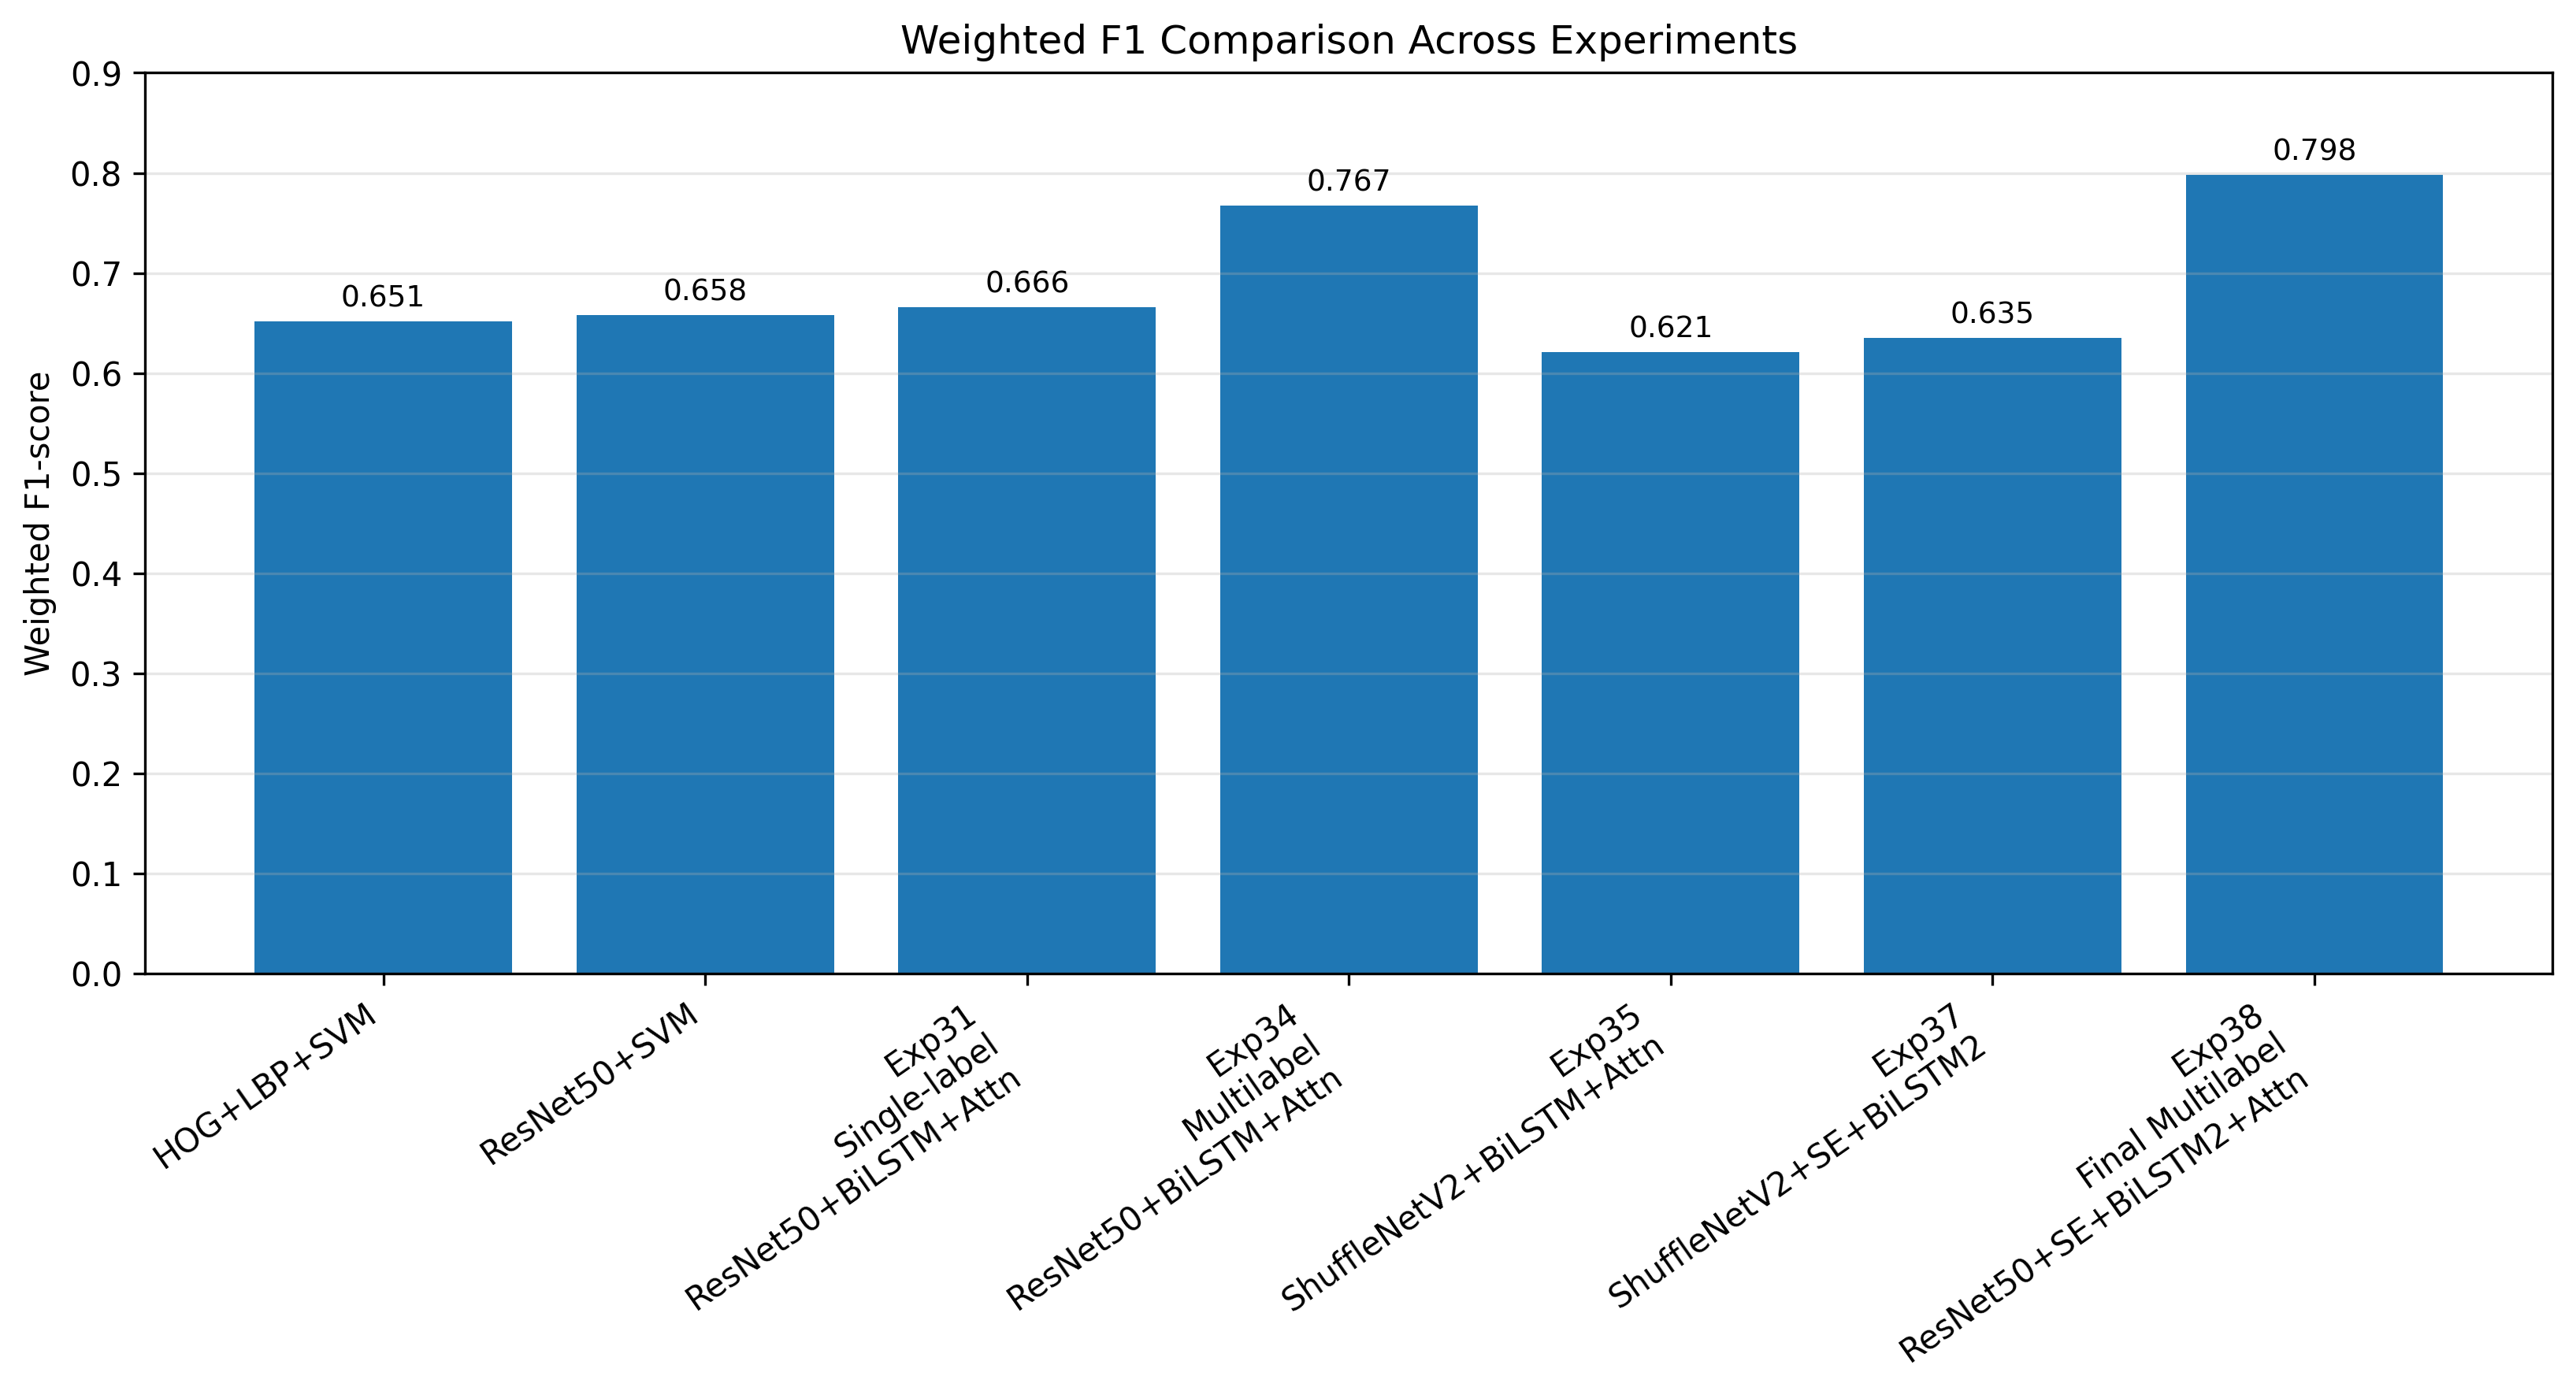
\includegraphics[width=0.92\textwidth]{Figures/fer_weighted_f1_comparison.png}
    \caption{Weighted F1 across the two traditional baselines and the strongest single-label and multilabel deep models. Weighted F1 puts more mass on the engagement label and is therefore closer between models than Macro F1, but the chosen multilabel system (Exp~38) still reaches the highest Weighted F1 ($0.80$), which means that even when the dominant class is given more weight, the proposed system is at least as good as the traditional and single-label baselines.}
    \label{fig:fer_weighted_f1_comparison}
\end{figure}

\subsection{Comparison with Prior FER Work on DAiSEE}\label{sec:results_fer_literature}

Prior FER work on DAiSEE is dominated by single-label engagement classifiers. Most of these works simplify DAiSEE to a four-class engagement task (engagement levels $0$--$3$) and report multiclass top-1 accuracy on the official test split \cite{gupta_daisee_2016,abedi_improving_2021,mehta_three-dimensional_2022,santoni_convolutional_2023,shiri_detection_2024,su_leveraging_2024,liu_dynamic_nodate,asaju_adaptive_2022,tulsani_realtime_2025,aly_revolutionizing_2025}. A direct head-to-head comparison between those engagement-only accuracies and the multilabel Macro F1 reported in this thesis is therefore not fair: the two solve different problems, with different denominators, and a $4$-class engagement classifier never has to deal with the ``boredom and frustration must be detected at the same time'' case. For this reason, the comparison in this section is qualitative and focuses on \emph{architectural choices}, not on numbers.

The closest design family in the literature is the one that combines a CNN backbone with a recurrent or attention-based temporal model. ResNet50~+~BiLSTM-style pipelines are reported in \cite{asaju_adaptive_2022,asaju_affects_2021,tulsani_realtime_2025,shiri_detection_2024}, and they form the empirical evidence for the choice of ResNet50 and BiLSTM in this thesis. ResNet~+~TCN pipelines are studied in \cite{abedi_improving_2021}, which is the same backbone family used here but with a temporal convolutional head instead of a BiLSTM; the present thesis explored this option in Exp~25 (ResNet50~+~CBAM~+~TCN) and Exp~30 (ResNet50~+~CBAM~+~3D~CNN) but found that the BiLSTM family is more stable on the small batch size used here. Three-dimensional spatiotemporal architectures with self-attention are studied in \cite{mehta_three-dimensional_2022,liu_dynamic_nodate}, and were explored in this thesis in Exp~19, Exp~27 and Exp~30; in our setting, the 3D variants did not reach the Macro F1 of the BiLSTM~+~temporal attention design. Transformer-based temporal models are studied in \cite{su_leveraging_2024,liu_dynamic_nodate} and were explored in Exp~11 and Exp~15; their performance was below the BiLSTM~+~temporal attention runs in our protocol, which is consistent with the observation in recent reviews that transformers tend to underperform BiLSTMs on DAiSEE-sized datasets without large-scale pretraining \cite{lek_academic_2023,vistorte_integrating_2024}.

CBAM-based attention modules are studied in \cite{aly_revolutionizing_2025,liu_dynamic_nodate} and were explored in this thesis in Exp~25 and Exp~30. SE attention is the channel-only variant of CBAM and is also used in \cite{aly_revolutionizing_2025}; the chosen final model uses SE rather than full CBAM because SE is lighter and combined more cleanly with the BiLSTM~+~temporal attention pipeline. Imbalance-aware training, with weighted loss or controlled oversampling, is recommended by \cite{santoni_convolutional_2023,abedi_improving_2021,rianto_engagement_2025} and is one of the dominant lessons of the architecture-selection experiments in this chapter, as discussed in Section~\ref{sec:results_fer_arch_selection}. Per-label threshold tuning, recommended by \cite{rianto_engagement_2025,mehta_three-dimensional_2022}, is also used here and is one of the most cost-effective interventions in our pipeline.

A second observation from the literature is that very few DAiSEE works report a true \emph{multilabel} four-state evaluation. Most engagement-focused works simplify the task to a single-label four-class engagement classifier, which is easier than predicting four overlapping binary labels \cite{abedi_improving_2021,mehta_three-dimensional_2022,su_leveraging_2024}, and the works that consider multilabel formulations focus on engagement plus one or two additional states rather than all four \cite{rianto_engagement_2025,fu_integrating_2025,asaju_adaptive_2022}. The proposed thesis pipeline is therefore positioned in a deliberately harder corner of the DAiSEE design space: it commits to all four DAiSEE labels at once, with a multilabel sigmoid head, weighted BCE, controlled oversampling and per-label thresholds. This is the configuration that is needed for downstream adaptation, because the adaptation module of Section~\ref{sec:method_integration} consumes the full four-dimensional emotion vector, not a single dominant label.

A summary of how the proposed system relates to prior FER work on DAiSEE is given in Table~\ref{tab:fer_lit_compare}. The table is intentionally architectural rather than numerical, in line with the consistency rule of Section~\ref{sec:results_fer_scope}.

\begin{table}[H]
\centering
\small
\caption{Architectural comparison with prior FER work on DAiSEE. ``ML'' indicates whether the work reports a true multilabel four-state evaluation (\textsc{yes}) or a single-label engagement-only formulation (\textsc{no}). ``RT'' indicates whether the work targets real-time / lightweight deployment.}
\label{tab:fer_lit_compare}
\begin{tabular}{p{3.4cm}p{3.5cm}p{3.6cm}cc}
\toprule
\textbf{Work} & \textbf{Backbone} & \textbf{Temporal/Attention} & \textbf{ML} & \textbf{RT} \\
\midrule
Gupta et al.\ \cite{gupta_daisee_2016}                & C3D / I3D            & 3D CNN                          & \textsc{yes} & \textsc{no}  \\
Abedi \& Khan \cite{abedi_improving_2021}             & ResNet               & TCN                             & \textsc{no}  & \textsc{no}  \\
Mehta et al.\ \cite{mehta_three-dimensional_2022}     & 3D DenseNet          & 3D self-attention               & \textsc{no}  & \textsc{no}  \\
Su et al.\ \cite{su_leveraging_2024}                  & CNN + Transformer    & part-and-sensitive attention    & \textsc{no}  & \textsc{no}  \\
Asaju \& Vadapalli \cite{asaju_adaptive_2022}         & CNN                  & BiLSTM                          & \textsc{yes} & partial      \\
Liu et al.\ \cite{liu_dynamic_nodate}                 & CNN + AGA            & differential temporal transformer & \textsc{no} & \textsc{no}  \\
Aly \cite{aly_revolutionizing_2025}                   & ResNet50 + CBAM      & TCN                             & \textsc{no}  & \textsc{yes} \\
Shiri et al.\ \cite{shiri_detection_2024}             & EfficientNetV2-L     & RNN                             & \textsc{no}  & \textsc{no}  \\
Santoni et al.\ \cite{santoni_convolutional_2023}     & CNN                  & ---                             & partial      & partial      \\
Rianto et al.\ \cite{rianto_engagement_2025}          & graph-based CNN      & ---                             & partial      & partial      \\
\midrule
\textbf{This thesis} & \textbf{ResNet50 + SE} & \textbf{2-BiLSTM + temp.\ attn.} & \textbf{\textsc{yes}} & \textbf{\textsc{yes}} \\
\bottomrule
\end{tabular}
\end{table}

The two distinguishing features of the proposed pipeline relative to Table~\ref{tab:fer_lit_compare} are: (i) it is a true multilabel four-state model, and (ii) it is webcam-only and lightweight enough to run on a single consumer-grade GPU, in line with the deployment constraint stressed by recent educational FER reviews \cite{lek_academic_2023,florestiyanto_emotion_2024,vistorte_integrating_2024}.

\subsection{Discussion of FER Results}\label{sec:results_fer_discussion}

Three findings stand out from the FER experiments and are worth re-stating clearly.

The first finding is that, on DAiSEE, accuracy alone is misleading. The two SVM baselines reach $0.75$ and $0.76$ test accuracy by predicting almost only engagement; the strongest single-label deep model reaches $0.70$ accuracy with very low minority F1; and even the chosen multilabel model has per-label accuracy of $0.91$ on frustration despite an F1 of only $0.25$, because most clips are not frustrated. Macro F1 is the metric that exposes the difference between a useful FER model and one that has collapsed to the dominant label. Recent surveys of educational FER and of multilabel imbalance handling have argued for exactly this position \cite{lek_academic_2023,santoni_convolutional_2023,rianto_engagement_2025}, and the experiments in this chapter confirm it on DAiSEE.

The second finding is that the highest Macro F1 in the multilabel family comes from the combination of three concurrent imbalance-aware mechanisms: controlled oversampling at the data level, weighted BCE at the loss level, and per-label threshold tuning at the decision level. None of the three alone is enough. Plain BCE collapses to engagement (Exp~1, Macro F1 $0.251$). Weighted BCE alone, with a fixed threshold, only reaches $0.408$ (Exp~4). Aggressive sampling without threshold tuning over-corrects and produces $0.153$ (Exp~6). The full combination, plus a strong spatiotemporal backbone, reaches $0.453$ (Exp~38). The lesson is that imbalance has to be addressed jointly at every stage of the pipeline, not at a single isolated stage.

The third finding is that the temporal axis matters. Within the multilabel family, the two-layer BiLSTM with temporal attention (Exp~16, Exp~17, Exp~38) outperforms the last-frame readouts (Exp~8, Exp~9), the one-layer BiLSTM without attention (Exp~10, Exp~12), the temporal transformer with the same backbone (Exp~11), the 3D CNN with self-attention (Exp~19) and the 3D ResNet (Exp~14). The temporal attention layer is conceptually justified in Section~\ref{sec:method_temporal_attention}: it lets the network give more weight to the few frames that contain affect-relevant cues, and less weight to frames where the face is occluded, the head is turned, or the eyes are closed. The empirical results in Table~\ref{tab:fer_arch_selection_multilabel} are consistent with that explanation.

These three findings, taken together, justify the final architecture and the choice of the multilabel formulation, and connect the conceptual rationale of Section~\ref{sec:method_design_rationale} to the experimental evidence of this chapter.

The FER pipeline still has limitations, and they should be acknowledged honestly. Confusion and frustration F1 stay around $0.22$--$0.25$, which is well below engagement F1. Part of this is intrinsic to DAiSEE: confusion and frustration are sparse, ambiguous, and often suppressed in front of a webcam, and learners can be confused without showing any face cue at all. Per-label thresholds produce a high-recall, low-precision profile on the rare labels, which means that the model is good at not missing rare positives but not at being right when it predicts them. Multilabel exact-match accuracy is $0.342$, which is non-trivial but far from perfect, because each missed minority label takes the whole clip out of the exact-match set. Finally, the model is webcam-only, so any classroom condition that breaks DAiSEE-style framing, such as severe occlusion, strong side-lighting, or off-screen learners, is expected to degrade performance, which is consistent with what classroom-deployed FER reviews report \cite{lek_academic_2023,florestiyanto_emotion_2024,vistorte_integrating_2024}.

Despite these limitations, the chosen multilabel model is suitable as input for the adaptation module: it produces a stable four-dimensional emotion vector per clip, with non-zero F1 on every label, with per-label accuracies that are uniformly above chance, and with reproducible thresholds saved alongside the best validation checkpoint. The next part of this chapter, on the adaptation module, will reuse this exact emotion vector as one of the inputs to the policy.

\subsection{Summary of FER Findings}\label{sec:results_fer_summary}

In summary, on the DAiSEE test set, the proposed FER model reaches a Macro F1 of $0.453$, a Weighted F1 of $0.798$, a Micro F1 of $0.724$, a Samples F1 of $0.746$, and an exact-match accuracy of $0.342$, with per-label F1 of $0.36$, $0.97$, $0.22$ and $0.25$ on boredom, engagement, confusion and frustration. This is the best multilabel result in the architecture-selection experiments, achieved by a ResNet50~+~SE~+~two-layer BiLSTM~+~temporal attention pipeline trained with weighted BCE plus controlled oversampling on $24$-frame clips, and decoded with per-label thresholds tuned on the validation split. The result is supported by ablations along five axes (imbalance handling, sampling-vs-loss interaction, backbone, temporal module, decision rule), by a comparison with traditional handcrafted-feature baselines, and by an architectural comparison with prior FER work on DAiSEE. Part~II of this chapter, on the adaptation module, builds on this FER output.

% =====================================================================
% PART II — ADAPTATION MODULE RESULTS AND DISCUSSION
% =====================================================================

\section{Adaptation Module Results and Discussion}\label{sec:results_adapt_part}

\subsection{Introduction to Adaptation Results}\label{sec:results_adapt_intro}

The adaptation module answers an operational question: \emph{given a compact student state that includes knowledge, engagement, continuous affect scalars, and a discrete emotion label, which pedagogical action should an automated tutor take next?} The module was trained and evaluated inside a synthetic Gymnasium environment (\texttt{StudentEnv}) with a population of $N=10{,}000$ simulated student profiles, action masking for safety, and a multi-term shaped reward (Section~\ref{sec:method_reward}). Five decision policies were compared: Maskable Proximal Policy Optimization (PPO) as the primary learner, Deep Q-Network (DQN), a LinUCB\,+\,DQN hybrid (\emph{Bandit+DQN}), a hand-crafted rule-based tutor, and a random legal-action baseline.

\textbf{Scope of evidence.} All quantitative RL results reported in this part use \textbf{simulator-derived affect states} (\texttt{USE\_REAL\_FER=False}). The \texttt{FERAdapter} maps frustration, confusion, and boredom thresholds to a discrete \texttt{emotion\_id}; it does \emph{not} consume live webcam predictions from the DAiSEE-trained FER model during training or evaluation. The FER results in Part~I therefore evaluate \emph{perception accuracy} on DAiSEE; the adaptation results evaluate \emph{control quality under synthetic affect}, with architectural readiness for future FER integration (Section~\ref{sec:method_integration}). No claim is made that the RL policies were improved by real FER outputs, nor that simulator gains transfer to human classrooms without further study.

The comparison goals are threefold: (i)~identify which learning algorithm best optimizes the designed reward under masking and equal reward weights; (ii)~test whether the discrete \texttt{emotion\_id} dimension adds value beyond the continuous affect scalars already present in the observation; and (iii)~characterize failure modes, variance across seeds, and threats to validity so that positive simulator findings are not over-interpreted.

\subsection{Experimental Setup Overview}\label{sec:results_adapt_setup}

Table~\ref{tab:adapt_experiment_setup} summarizes the protocol aligned with Section~\ref{sec:method_eval} and \texttt{RL\_Module/config.py}. Each RL algorithm was trained for \texttt{TOTAL\_TIMESTEPS = 50{,}000} environment steps per random seed, then evaluated for \texttt{EVAL\_EPISODES = 1{,}000} episodes with deterministic action selection (PPO) or greedy/$\epsilon$-minimal policies (DQN). Ten independent seeds were used (\texttt{SEEDS = [42, 0, 1, 7, 13, 21, 99, 100, 200, 314]}); reported aggregates are means across seeds, with standard deviations or $95\%$ confidence intervals where noted. Rule-based and random agents skip gradient updates but follow the same evaluation episodes and seeds.

\begin{table}[H]
\centering
\caption{Adaptation-module experimental setup (main runs).}
\label{tab:adapt_experiment_setup}
\begin{tabular}{ll}
\toprule
\textbf{Setting} & \textbf{Value} \\
\midrule
Environment API & Gymnasium \texttt{StudentEnv}, max horizon $50$ steps \\
Synthetic population & $10{,}000$ profiles; uniform personality sampling \\
Training budget / seed & $50{,}000$ timesteps \\
Evaluation episodes / seed & $1{,}000$ \\
Random seeds (main) & $10$ fixed integers \\
Primary learner & MaskablePPO (\texttt{sb3\_contrib}), MLP $[256,256,256]$ \\
Affect input (main runs) & Simulator thresholds $\rightarrow$ \texttt{emotion\_id}; \texttt{USE\_REAL\_FER=False} \\
Framework & Stable-Baselines3 $\geq 2.2$, PyTorch \\
Reproducibility & \texttt{set\_all\_seeds} for Python, NumPy, PyTorch \\
Hardware & Single-machine CPU/GPU [TODO: specify GPU model used for final runs] \\
\bottomrule
\end{tabular}
\end{table}

The emotion ablation (Section~\ref{sec:results_adapt_ablation}) re-trains PPO only, with \texttt{ablation\_no\_emotion=True} forcing observation dimension $5$ (\texttt{emotion\_id}) to zero while dimensions $0$--$4$ (knowledge, engagement, frustration, confusion, boredom) remain unchanged. Sensitivity analysis (Section~\ref{sec:results_adapt_sensitivity}) uses a reduced budget of $5{,}000$ timesteps and $50$ evaluation episodes per factorial cell on seed $42$ only; it is reported as a robustness \emph{probe}, not as a definitive hyperparameter study.

\subsection{Evaluation Metrics}\label{sec:results_adapt_metrics}

Adaptation quality is measured with complementary metrics. None of them alone constitutes proof of educational effectiveness on real learners; together they characterize policy behavior \emph{inside the simulator} under the reward and masking rules defined in the methodology.

\paragraph{Mean episode reward.} The sum of per-step rewards $r_t$ over an episode, averaged across evaluation episodes and seeds. Because $r_t \in [-1,1]$ after clipping, cumulative reward reflects both knowledge progress and affect penalties/bonuses. This is the primary RL optimization target.

\paragraph{Normalized learning gain.} Hake-style gain on remaining knowledge headroom (Equation~\eqref{eq:delta_k_norm}), aggregated from episode start to end. High values indicate large relative knowledge growth within a session. This metric can \emph{disagree} with mean reward when affect penalties dominate or when policies terminate early.

\paragraph{Success rate.} Fraction of episodes with final knowledge $k>0.8$, frustration $f<0.3$, and confusion $c<0.4$ (Section~\ref{sec:method_eval}). [TODO: insert per-algorithm success rates from \texttt{logs/summary.csv} if regenerated before final submission.]

\paragraph{Dropout rate.} Fraction of episodes ending in frustration-driven dropout ($\geq 5$ consecutive steps with persistent frustration flag). Lower is generally preferable under the simulator's harm model.

\paragraph{Rule-consistency rate (formerly ``adaptation accuracy'').} Post-hoc fraction of steps where the chosen action belongs to \texttt{BEST\_ACTION\_MAP} for the current \texttt{emotion\_id}. This map is a \textbf{design-time expert table used only for evaluation}; it is \textbf{not} in the reward and \textbf{not} used during training. The metric measures alignment with hand-specified emotion--action heuristics, \textbf{not} ground-truth pedagogical correctness or human teacher approval. Throughout this chapter it is referred to as \emph{rule-consistency rate} to avoid implying educational validity.

\paragraph{Auxiliary diagnostics.} Episode length, action histograms, rolling reward standard deviation (convergence heuristic), and optional explainability JSONL traces (Figure~\ref{fig:rl_explainability}) support qualitative interpretation. Policy entropy during training is influenced by PPO's \texttt{ent\_coef = 0.01}.

\subsection{Algorithm Comparison: PPO, DQN, Rule-Based, and Random}\label{sec:results_adapt_algo_compare}

Table~\ref{tab:adapt_main_comparison} reports aggregated results from the unified thesis export (\texttt{thesis\_results.csv}). Figure~\ref{fig:rl_global_comparison} and Figure~\ref{fig:rl_mean_reward} visualize the same comparison; Figure~\ref{fig:rl_learning_gain} and Figure~\ref{fig:rl_rule_consistency} show learning gain and rule-consistency rate separately.

\begin{table}[H]
\centering
\caption{Main adaptation comparison over ten seeds ($1{,}000$ eval episodes per seed). Mean episode reward shown as mean $\pm$ std across seeds. Rule-consistency rate is the post-hoc \texttt{BEST\_ACTION\_MAP} match rate (not educational accuracy).}
\label{tab:adapt_main_comparison}
\begin{tabular}{lcccc}
\toprule
\textbf{Policy} & \textbf{Mean reward} & \textbf{Learning gain} & \textbf{Rule-consistency} & \textbf{Reward std} \\
\midrule
PPO (emotion-aware) & $3.596 \pm 0.112$ & $0.592$ & $0.315$ & $0.112$ \\
DQN                 & $1.749 \pm 0.850$ & $0.538$ & $0.179$ & $0.850$ \\
Bandit+DQN          & $1.748 \pm 0.852$ & $0.539$ & $0.179$ & $0.852$ \\
Random (legal)      & $1.730 \pm 0.071$ & $0.776$ & $0.299$ & $0.071$ \\
Rule-based          & $-1.532 \pm 0.061$ & $0.881$ & $0.257$ & $0.061$ \\
\bottomrule
\end{tabular}
\end{table}

\begin{figure}[H]
    \centering
    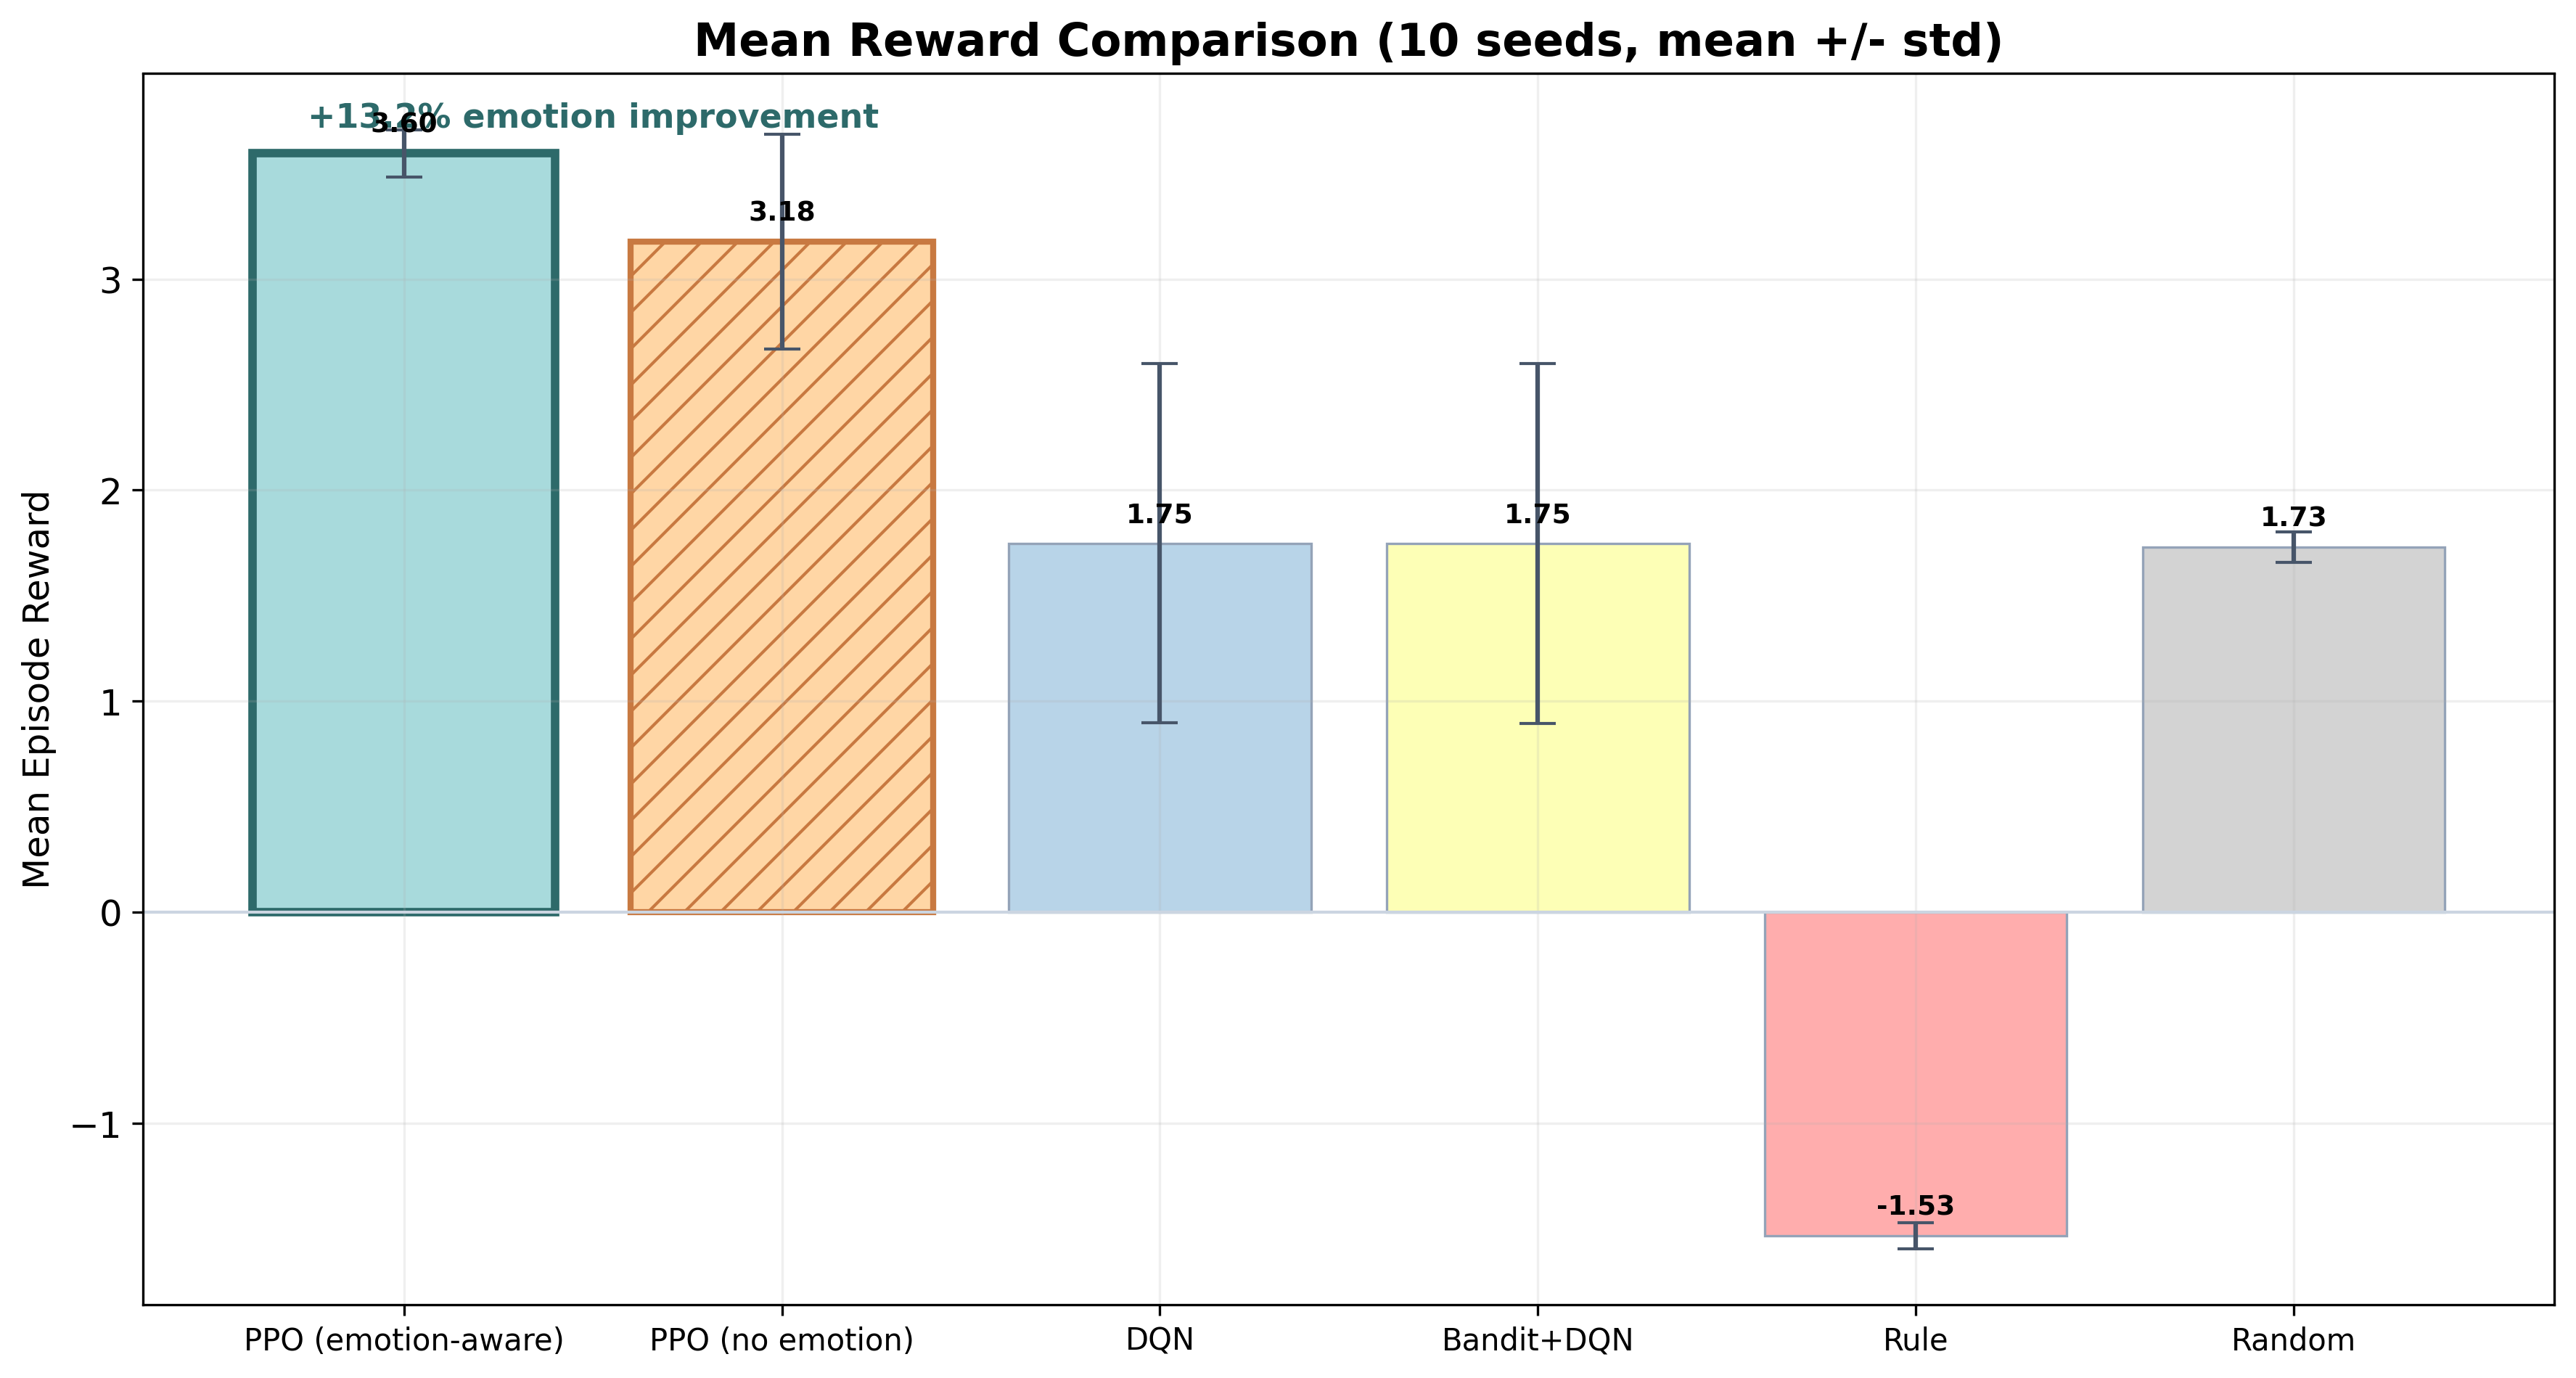
\includegraphics[width=0.95\textwidth]{Figures/global_comparison.png}
    \caption{Multi-metric comparison of all policies (thesis final suite). Bars aggregate ten seeds; error bars reflect cross-seed variability on mean episode reward. PPO dominates mean reward; rule-based and random policies show different trade-offs on learning gain versus reward.}
    \label{fig:rl_global_comparison}
\end{figure}

\begin{figure}[H]
    \centering
    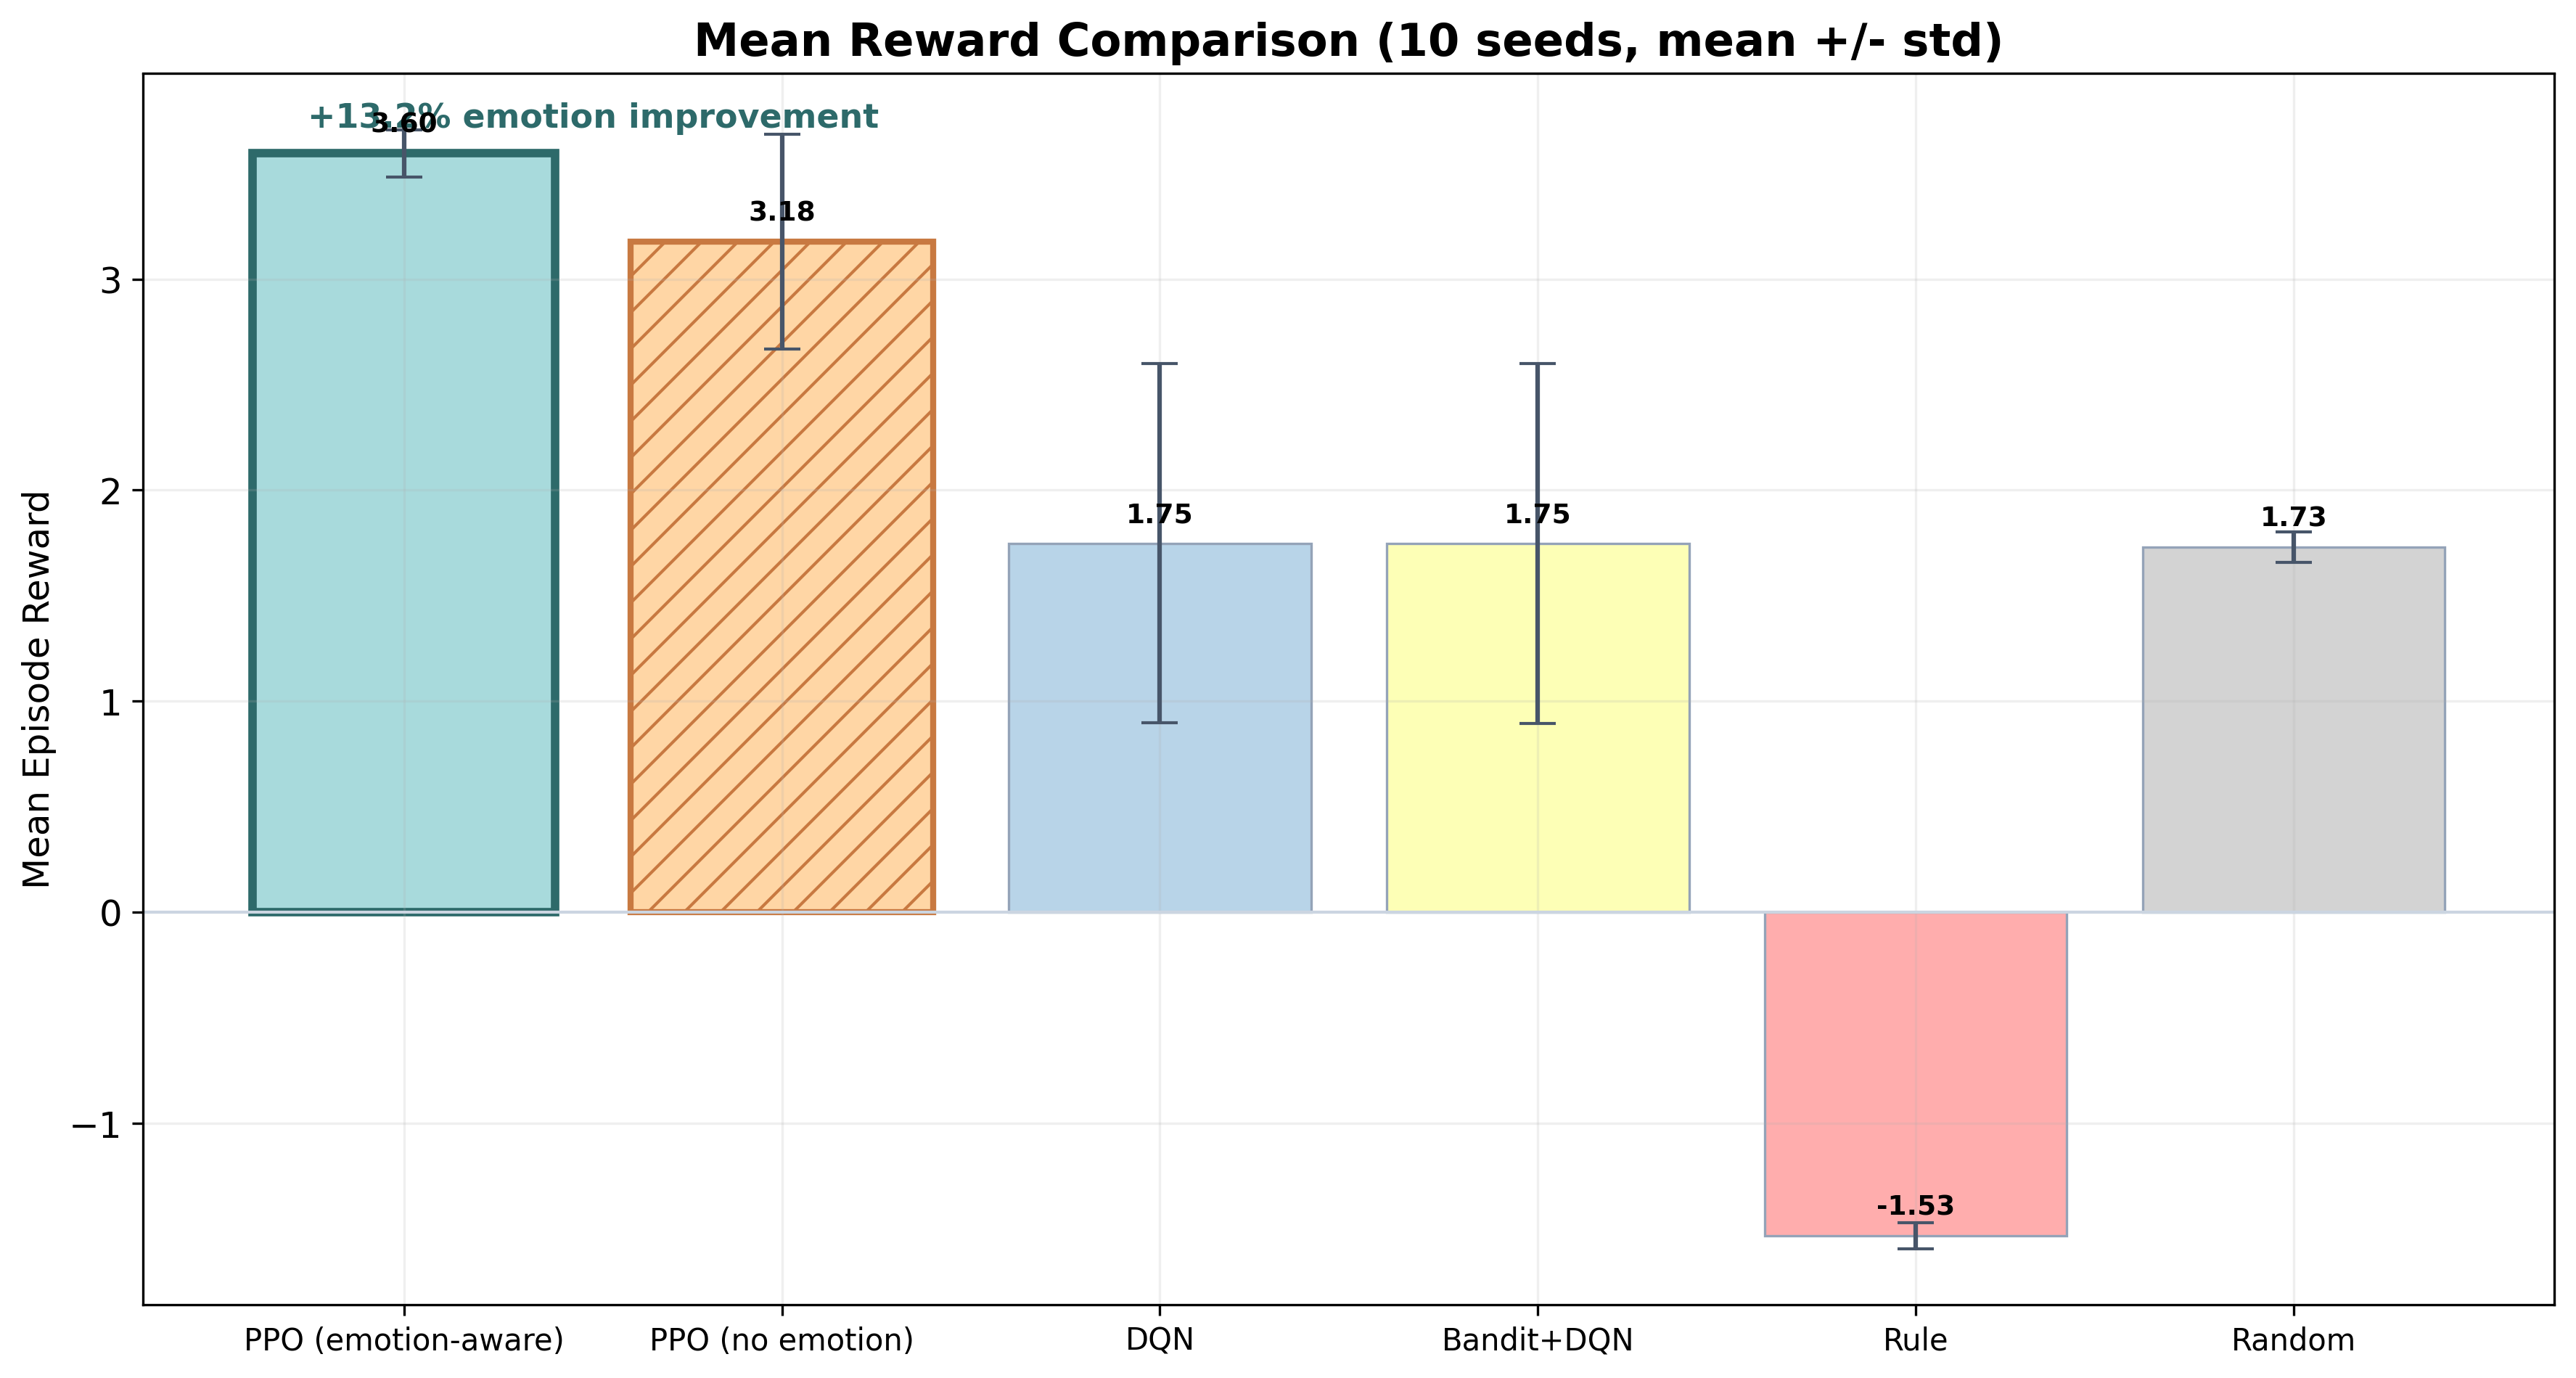
\includegraphics[width=0.88\textwidth]{Figures/mean_reward_comparison.png}
    \caption{Mean episode reward ($\pm$ std across seeds). PPO achieves the highest average return with relatively low variance ($\sigma \approx 0.11$), while DQN and Bandit+DQN exhibit high seed sensitivity ($\sigma \approx 0.85$). The rule-based policy yields negative mean reward because its fixed priority chain frequently violates the shaped reward (e.g., scaffolding when engagement is already low) even when knowledge rises.}
    \label{fig:rl_mean_reward}
\end{figure}

\begin{figure}[H]
    \centering
    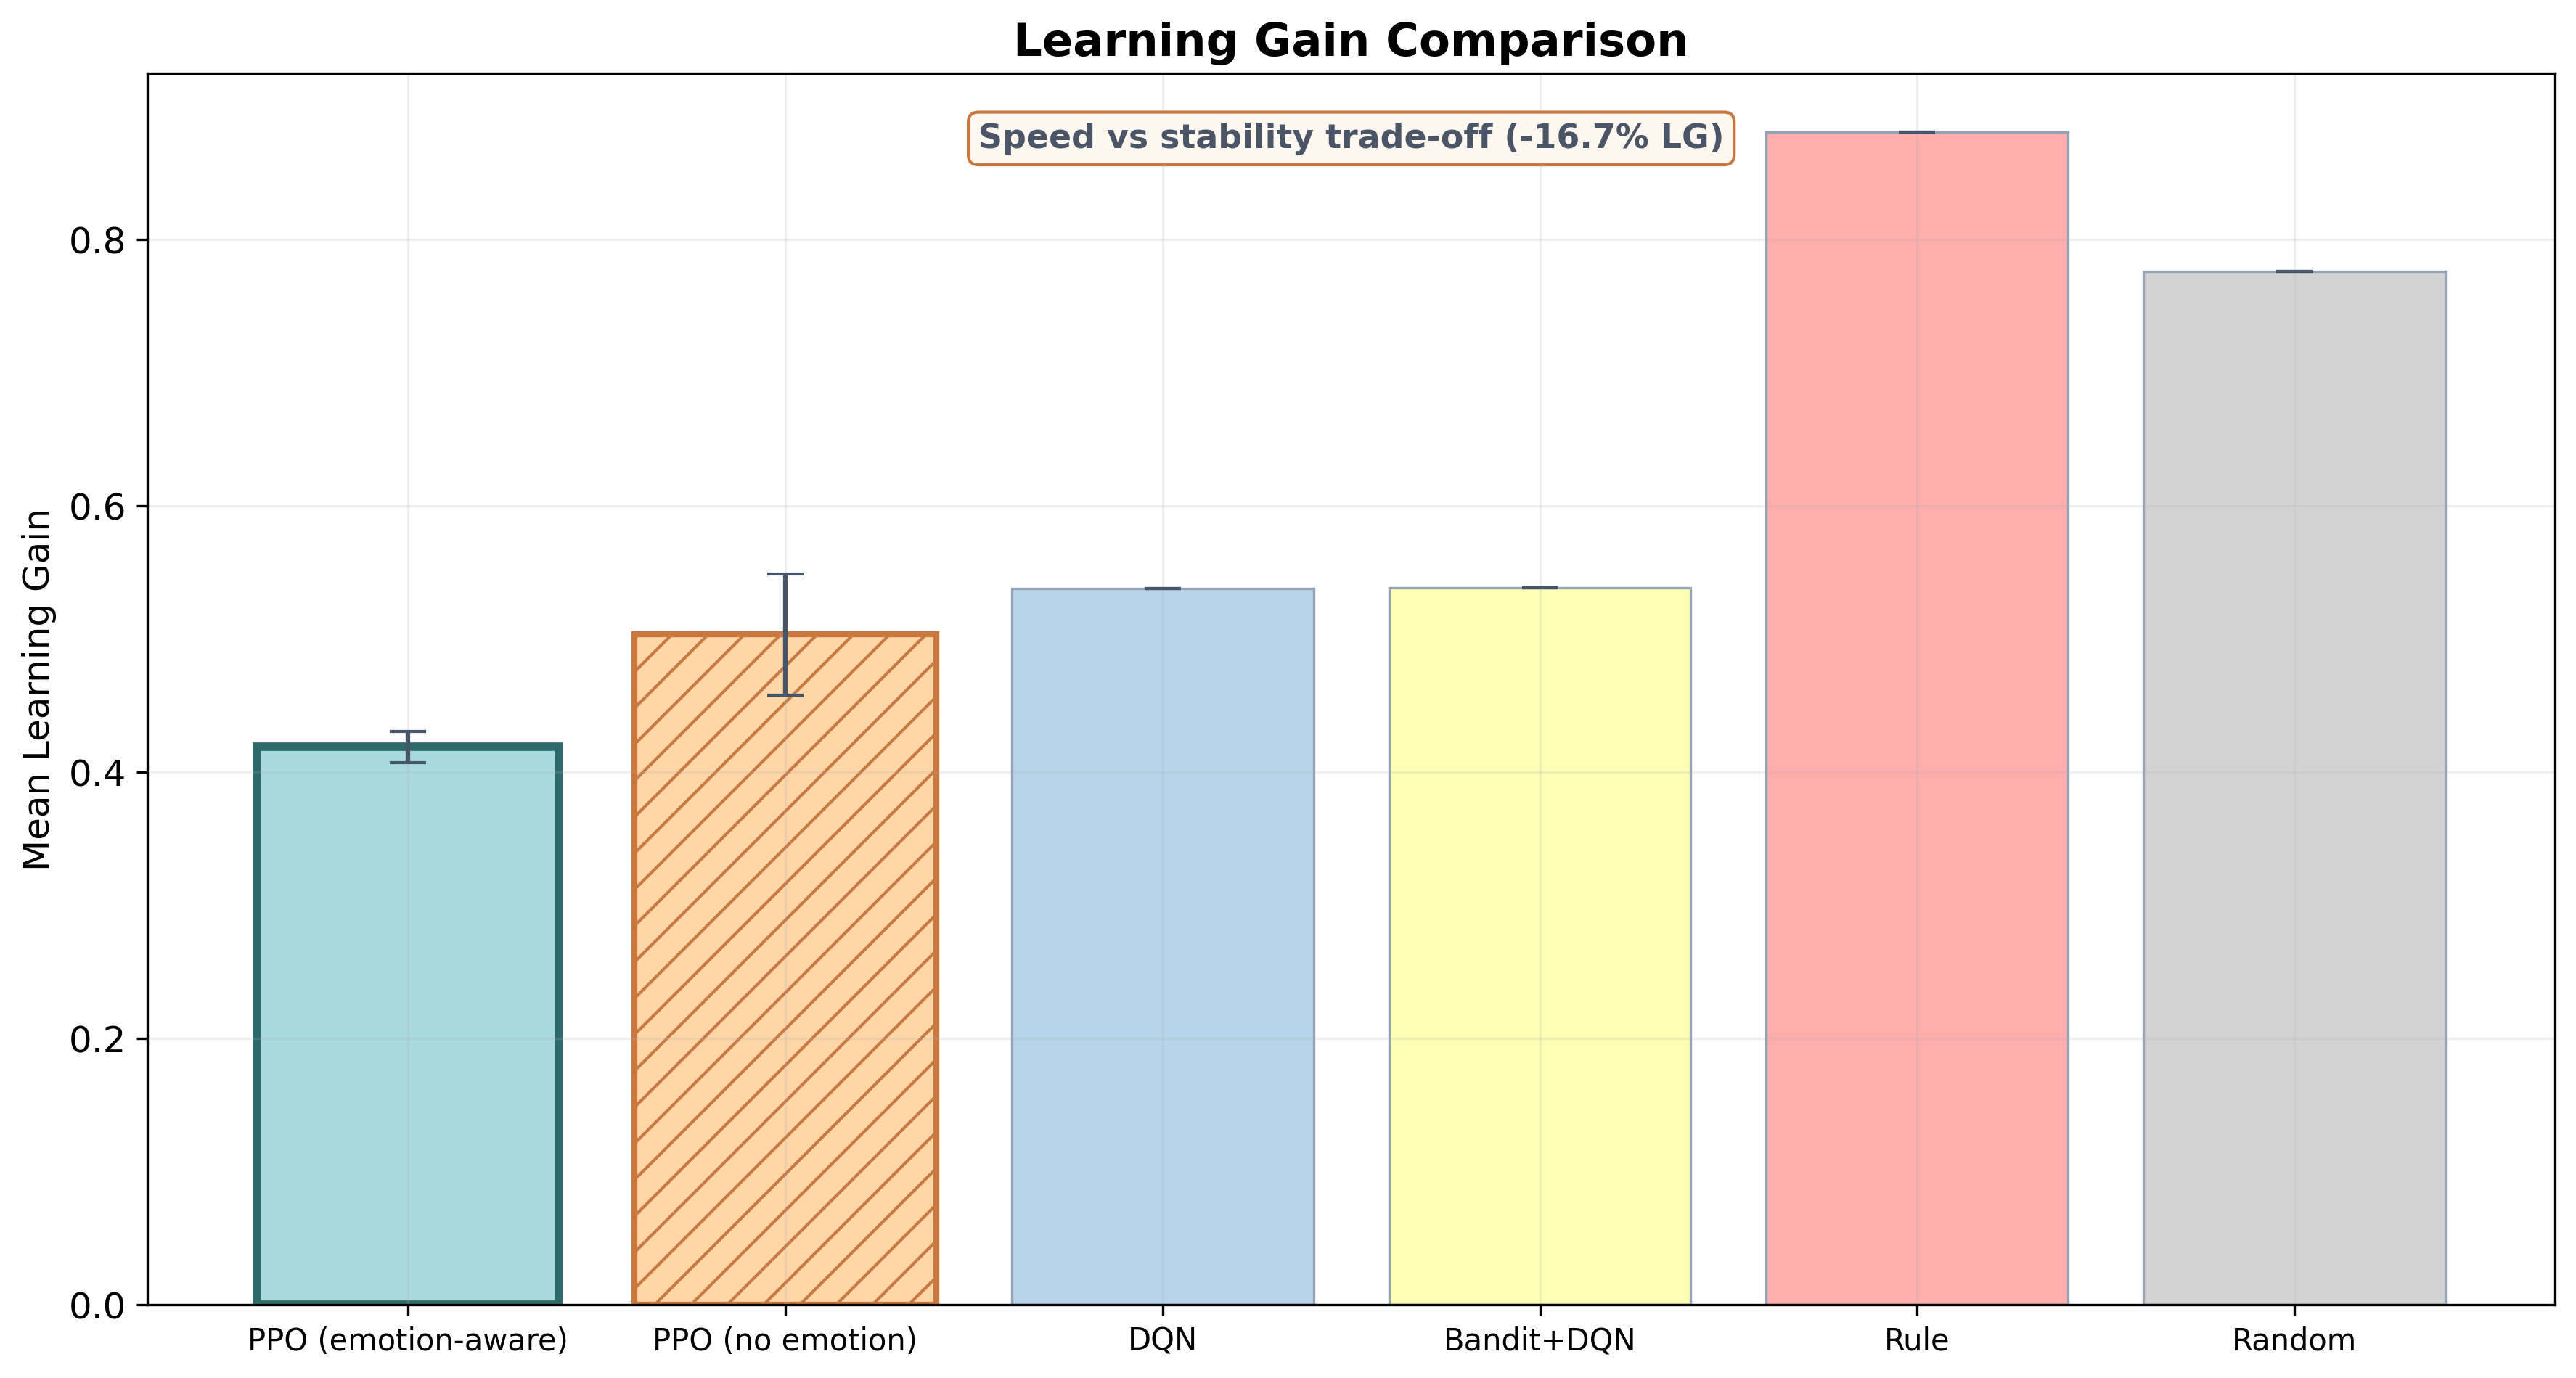
\includegraphics[width=0.88\textwidth]{Figures/learning_gain_comparison.png}
    \caption{Mean normalized learning gain. The rule-based tutor attains the highest learning gain ($0.881$) but the \emph{lowest} mean reward, illustrating metric conflict under shaped rewards. PPO achieves the best reward--gain compromise among learned policies; random exploration produces high gain with mediocre reward and rule-consistency.}
    \label{fig:rl_learning_gain}
\end{figure}

\begin{figure}[H]
    \centering
    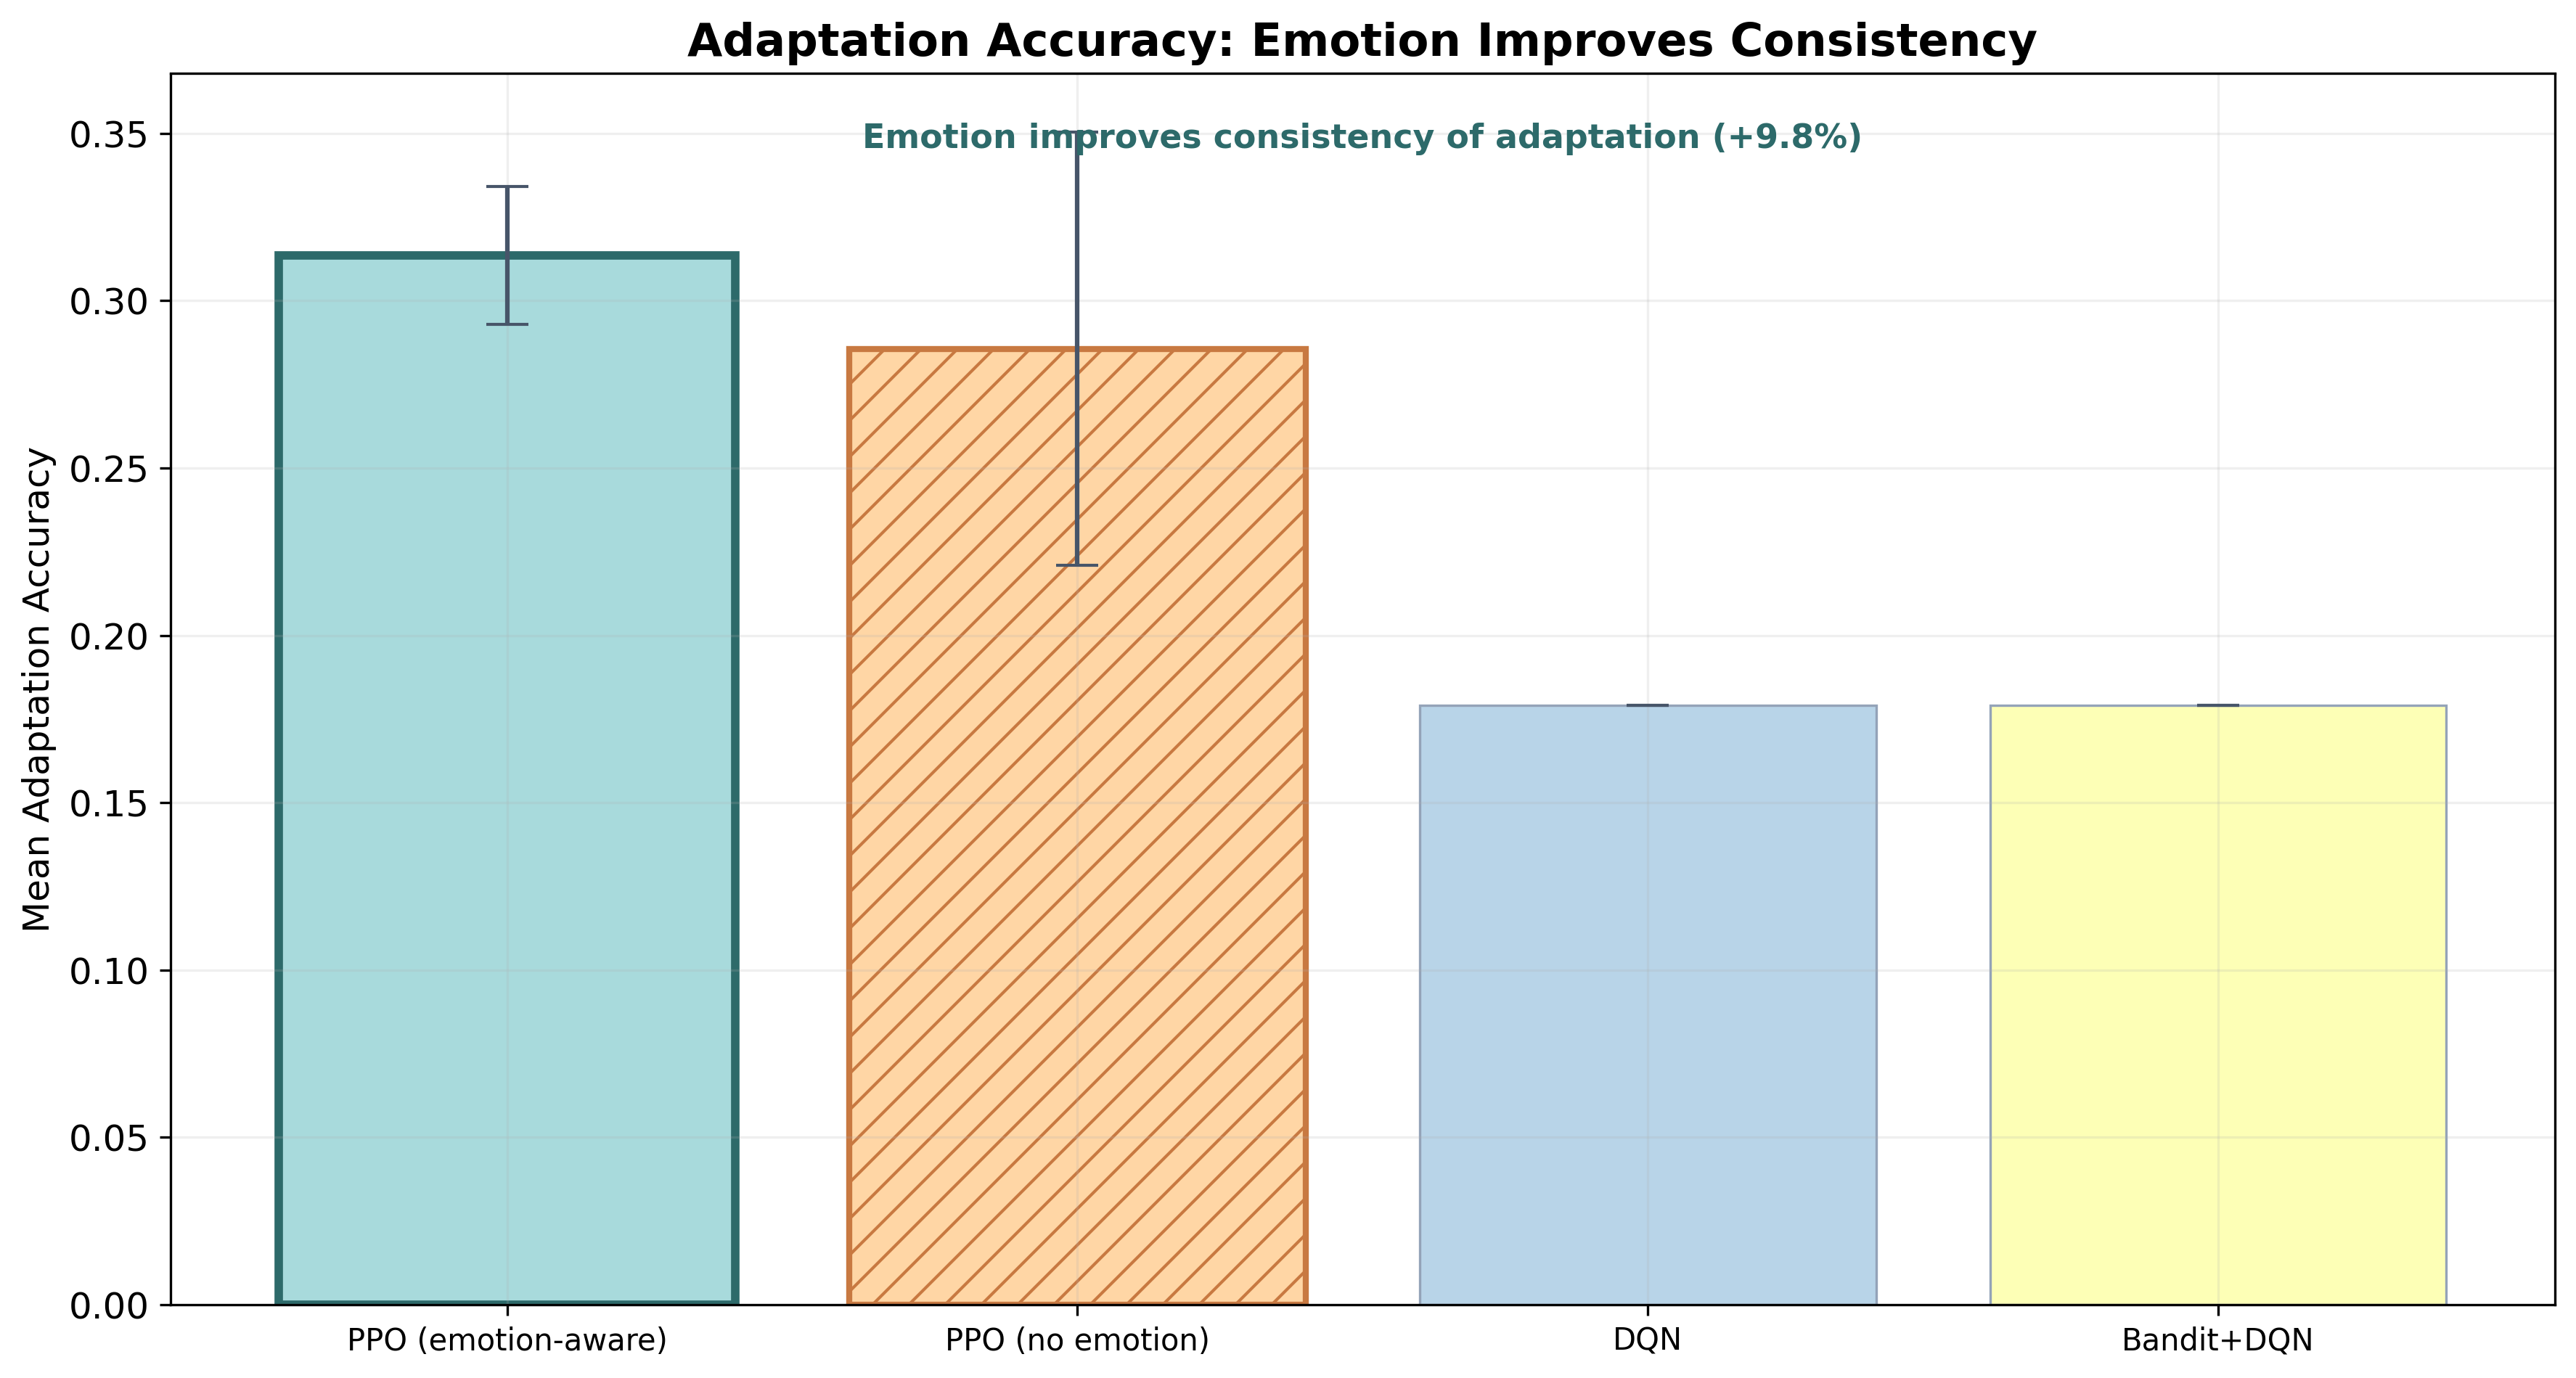
\includegraphics[width=0.88\textwidth]{Figures/adaptation_accuracy.png}
    \caption{Rule-consistency rate (post-hoc match to \texttt{BEST\_ACTION\_MAP}). PPO ($0.315$) exceeds DQN and the hybrid ($\approx 0.18$) but is only marginally above random ($0.299$), indicating that high reward is not reducible to mimicking the expert table.}
    \label{fig:rl_rule_consistency}
\end{figure}

\paragraph{PPO (MaskablePPO).} PPO achieves the highest mean episode reward ($3.596 \pm 0.112$) with the lowest cross-seed standard deviation among learned policies. Clipped surrogate updates, on-policy rollouts (\texttt{n\_steps = 2048}), and native action masking via \texttt{sb3\_contrib} avoid the illegal-action resampling path required by DQN. Under the evaluated conditions, PPO is the most \emph{stable} and \emph{reward-efficient} learner. Its learning gain ($0.592$) is lower than the rule-based and random baselines, which suggests the policy optimizes the full reward vector---including engagement and affect penalties---rather than knowledge alone.

\paragraph{DQN.} DQN reaches only $1.749 \pm 0.850$ mean reward with the lowest rule-consistency ($0.179$). Three mechanisms likely contribute. First, the smaller network ($[64,64]$) may underfit the six-dimensional state under a $50$k-step budget. Second, $\epsilon$-greedy exploration during the first $10\%$ of training injects noise that is not fully washed out by evaluation greediness. Third, \textbf{train/eval mismatch}: during training, \texttt{DQNSafeEnv} resamples illegal actions uniformly from the mask; during evaluation, invalid greedy choices are corrected differently. PPO never executes illegal actions in either phase. DQN's learning gain ($0.538$) remains respectable, so value learning captures some knowledge dynamics but fails to integrate affective costs into a high-return policy.

\paragraph{Rule-based baseline.} The static waterfall policy maximizes normalized learning gain ($0.881$) yet produces \textbf{negative} mean reward ($-1.532 \pm 0.061$). This is a central finding: hand-crafted rules can aggressively push knowledge upward while systematically incurring frustration, boredom, and wrong-answer penalties in the simulator. Rule-consistency ($0.257$) is not highest despite rules being written from the same emotion--action intuition as \texttt{BEST\_ACTION\_MAP}, because the waterfall ordering can select a ``reasonable'' emotion match that is still reward-suboptimal after masking and cooldowns.

\paragraph{Random legal-action baseline.} Uniform random choice over masked actions yields mean reward $1.730 \pm 0.071$ with remarkably high learning gain ($0.776$) and rule-consistency $0.299$. Low variance across seeds indicates that the environment's stochastic student dynamics, not policy brilliance, drive much of the knowledge trajectory. Random serves as a sanity check: PPO must beat chance on reward by a clear margin---which it does---but not on every secondary metric.

\subsection{PPO--Bandit--DQN Hybrid Results}\label{sec:results_adapt_hybrid}

The Bandit+DQN agent routes decisions through LinUCB when $|\Delta \texttt{emotion\_id}| \geq 1$, otherwise through DQN. Aggregated performance is virtually identical to DQN alone: mean reward $1.748 \pm 0.852$, learning gain $0.539$, rule-consistency $0.179$ (Table~\ref{tab:adapt_main_comparison}). The hybrid does not improve mean reward or stability relative to DQN; coordination overhead and context switching between two value estimates appear to offer no benefit within this simulator and sample budget.

A plausible explanation is that emotion changes are frequent enough that the bandit arm is selected often, but the LinUCB context $[\iota/3, f, b]$ is too coarse to outperform the DQN $Q$-function on the full state. Alternatively, both components are under-trained relative to PPO, so any hybrid advantage is below measurement noise ($\sigma \approx 0.85$). The hybrid should not be discarded for all future settings---richer contexts or pre-trained DQN features might help---but \textbf{under the evaluated conditions it is not supported as a stronger baseline than PPO.}

\subsection{Training Stability Analysis}\label{sec:results_adapt_stability}

Figure~\ref{fig:rl_robustness} plots cross-seed standard deviation of mean episode reward. PPO's seed-wise spread is an order of magnitude smaller than DQN's, confirming that on-policy clipping plus masking yields \emph{reproducible} policies across initializations. DQN and Bandit+DQN exhibit heavy-tailed seed outcomes: some seeds likely converge to mediocre $Q$-functions while others collapse.

\begin{figure}[H]
    \centering
    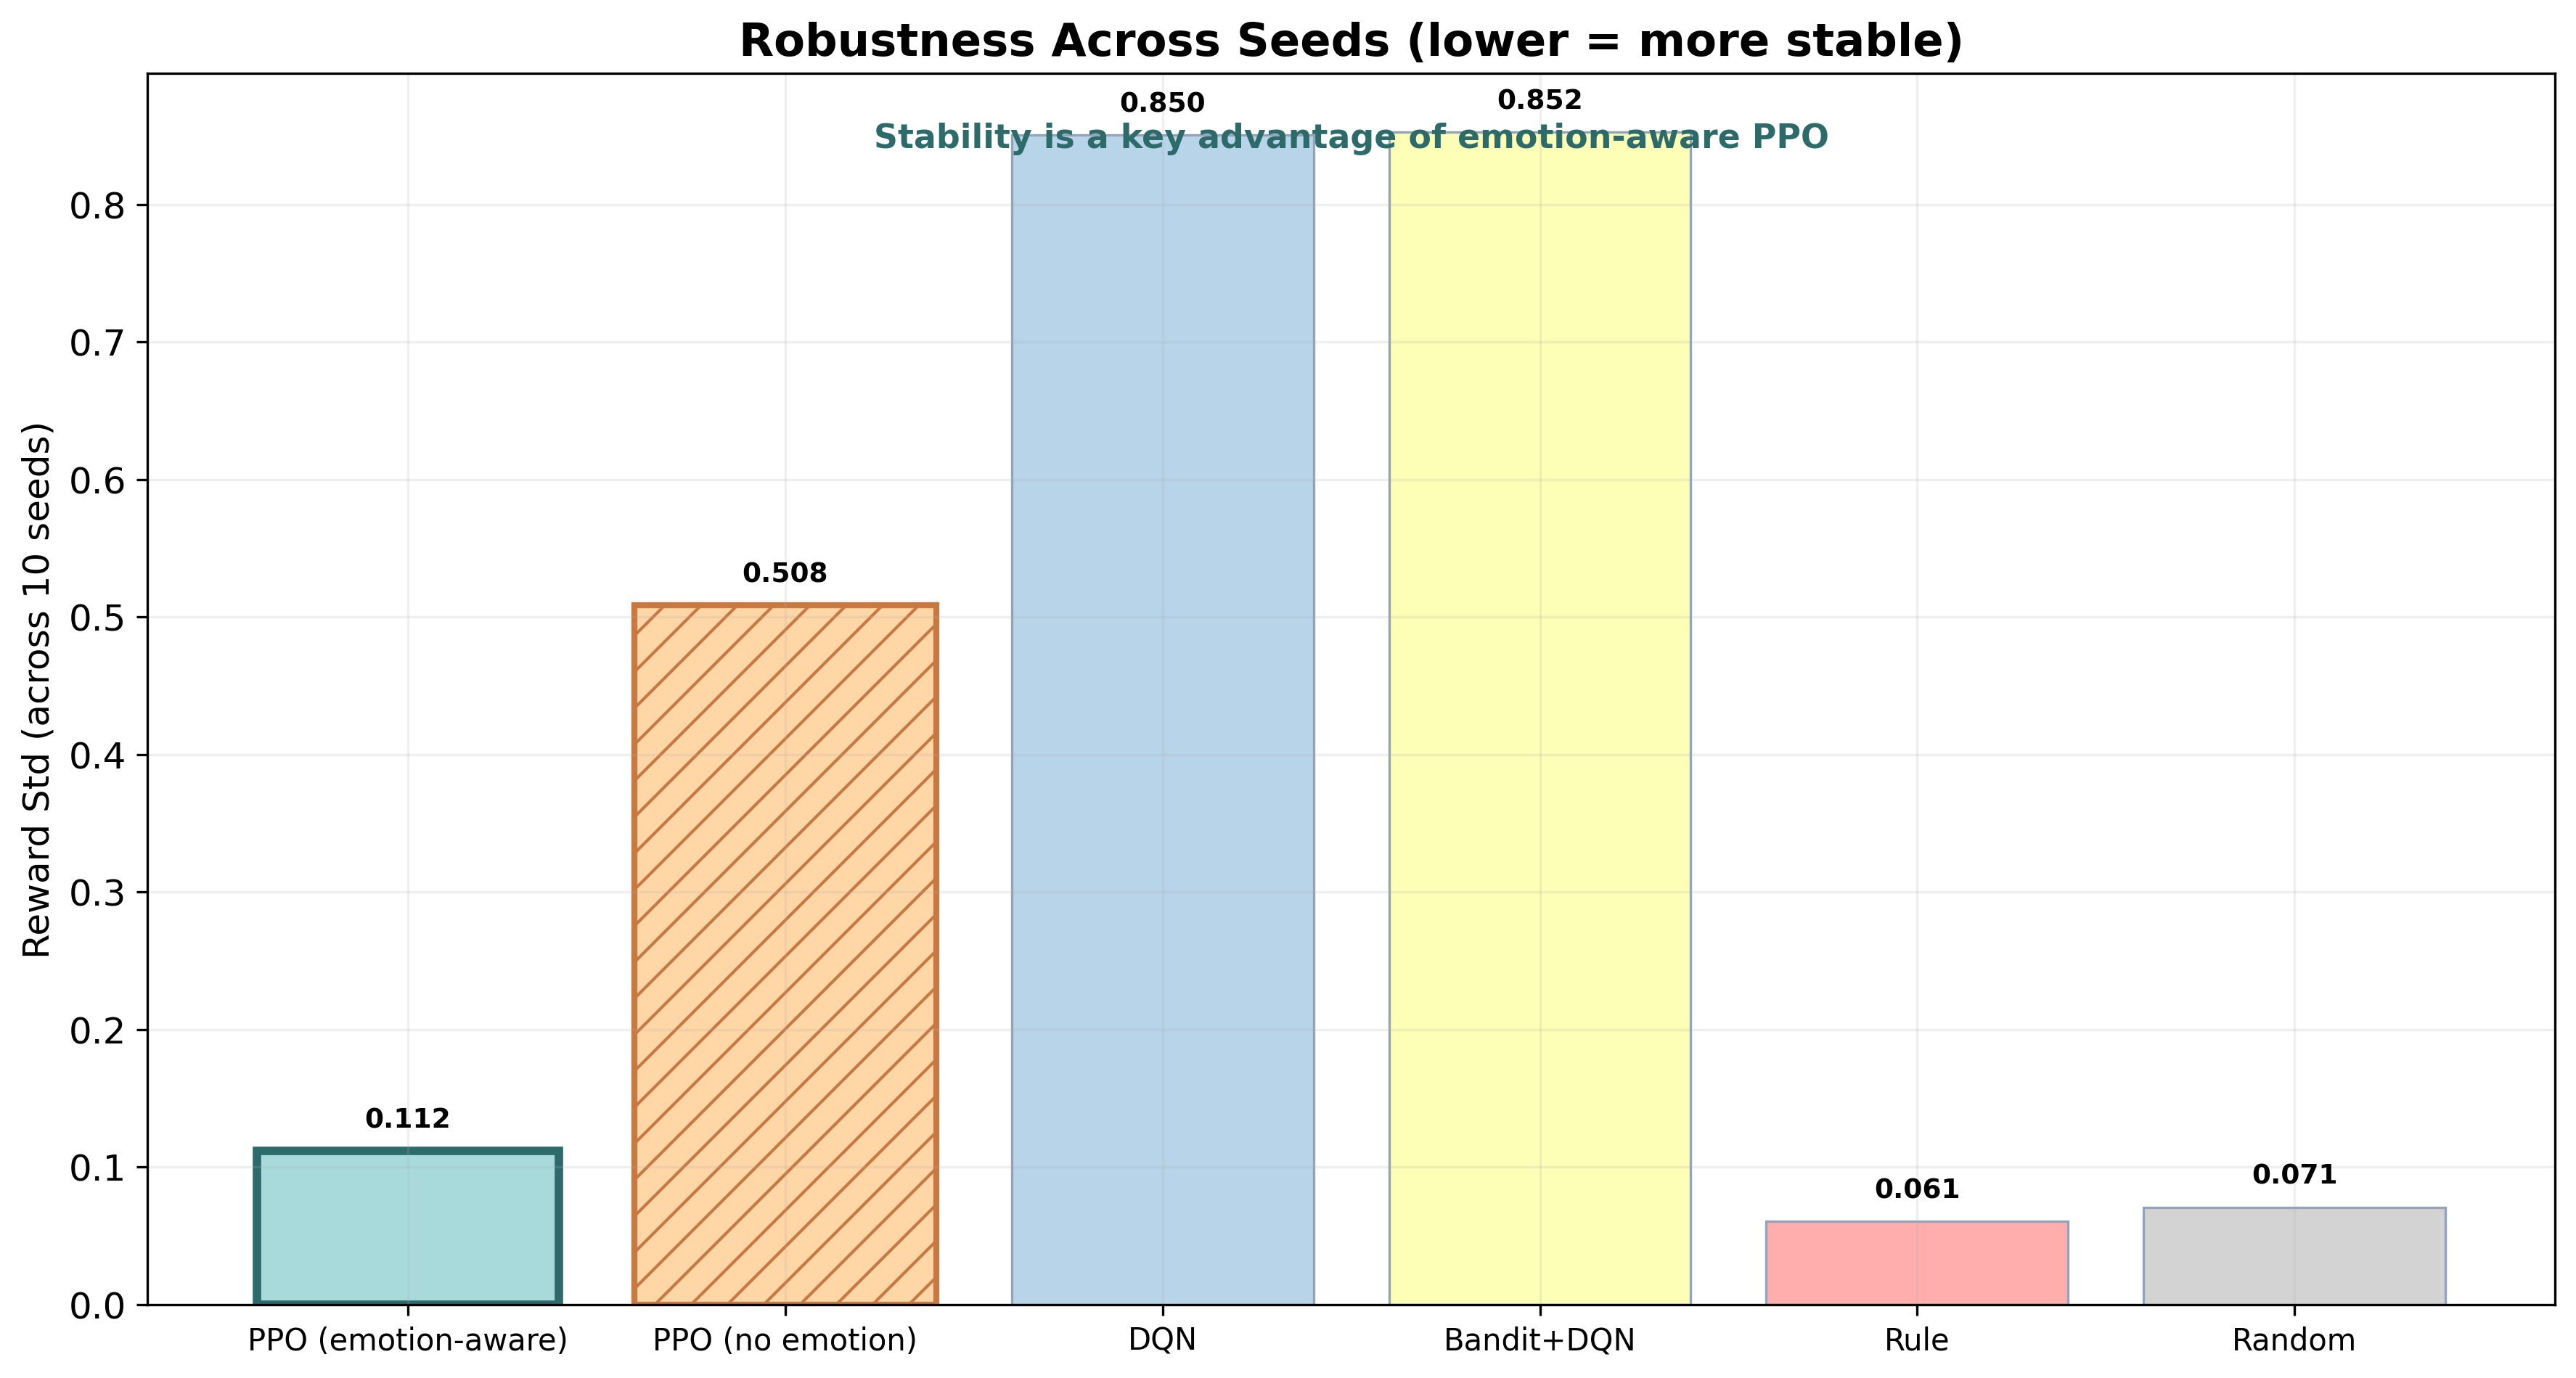
\includegraphics[width=0.85\textwidth]{Figures/robustness_std.png}
    \caption{Cross-seed standard deviation of mean episode reward (robustness). Lower is better. PPO shows the most stable replication; value-based baselines are seed-sensitive.}
    \label{fig:rl_robustness}
\end{figure}

Within training curves (Section~\ref{sec:results_adapt_learning_curves}), PPO typically exhibits smooth upward drift in rolling episode return, punctuated by short plateaus when the policy discovers masking-limited regions of the action space. DQN curves often oscillate: $\epsilon$-decay, target-network updates every $500$ steps, and off-policy replay with resampled illegal actions introduce non-stationarity. Entropy collapse was not systematically logged [TODO: insert TensorBoard policy entropy summary if exported]. Qualitatively, PPO retains stochasticity through \texttt{ent\_coef} until evaluation, which may prevent premature determinism on a single suboptimal action chain.

Reward shaping interacts with stability: the flow-zone bonus ($+1.0$ when all affect and knowledge thresholds align) creates sparse ``spikes'' that can accelerate learning but also encourage short-lived reward hacking (Section~\ref{sec:results_adapt_failures}). Clipping $r_t \in [-1,1]$ limits gradient explosions but compresses discrimination between good and excellent steps.

\subsection{Learning Curve Analysis}\label{sec:results_adapt_learning_curves}

Figure~\ref{fig:rl_learning_curves_all} overlays smoothed learning curves for all algorithms; Figure~\ref{fig:rl_learning_curves_ppo} zooms into PPO versus PPO-without-emotion ablation.

\begin{figure}[H]
    \centering
    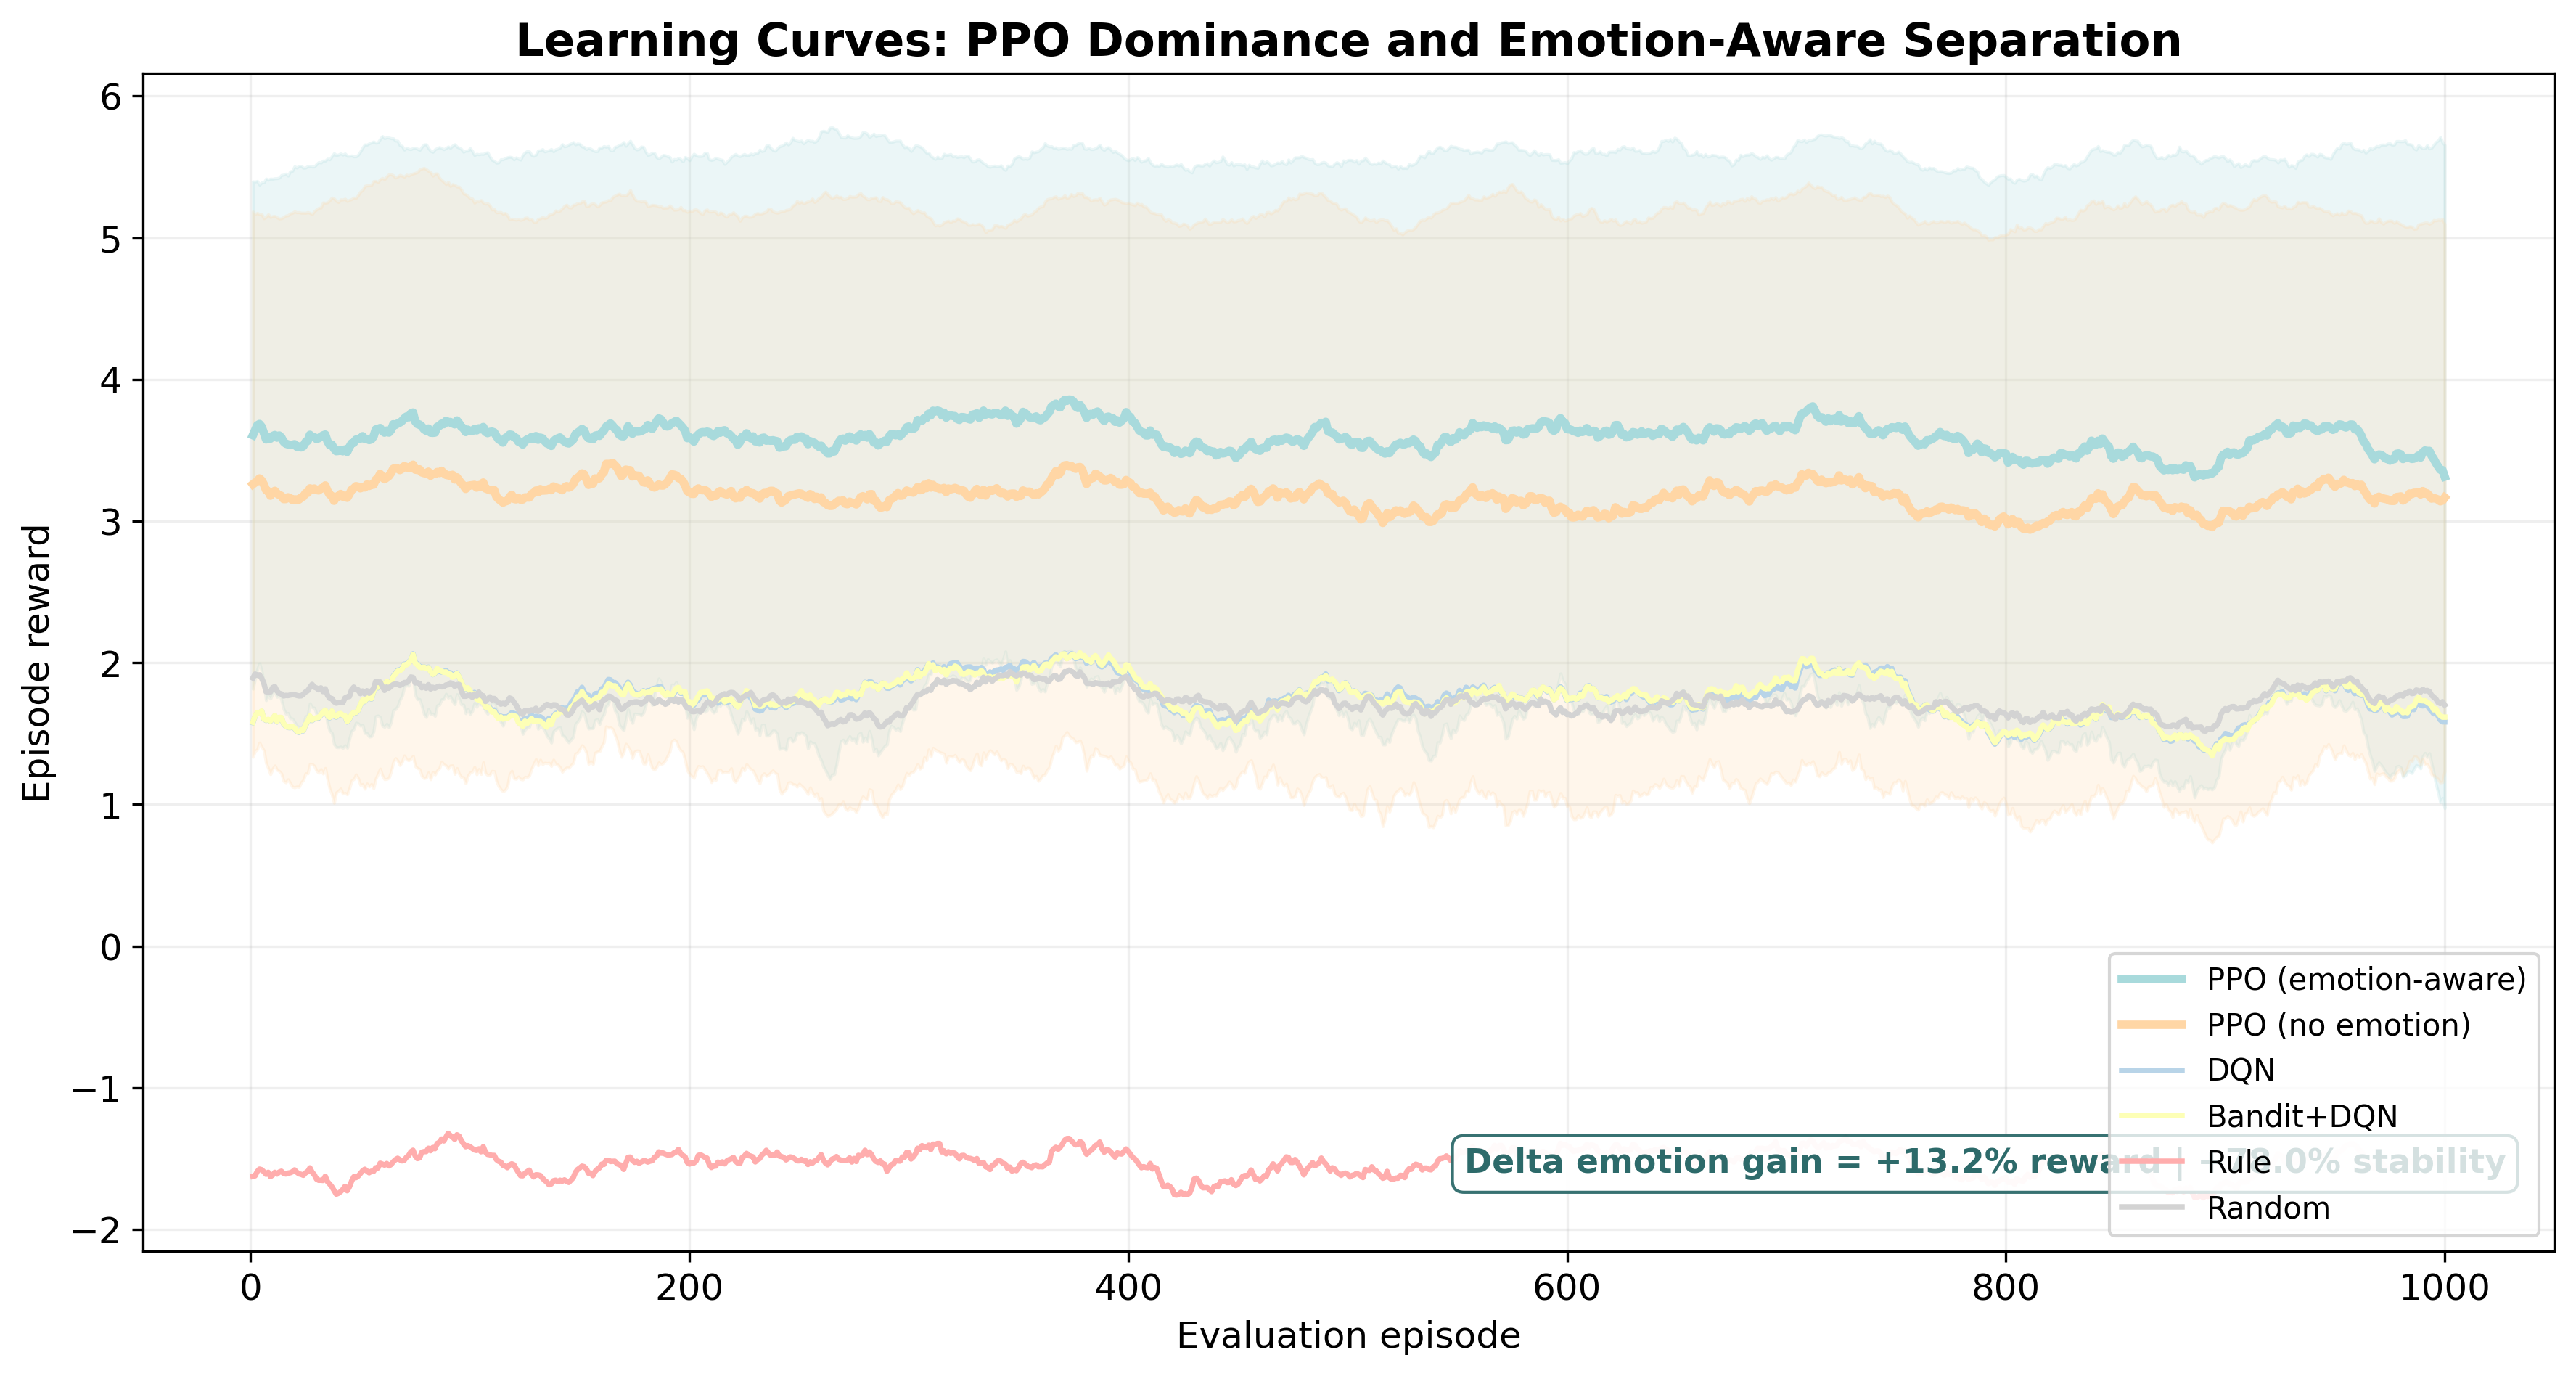
\includegraphics[width=0.95\textwidth]{Figures/learning_curves_all.png}
    \caption{Rolling mean episode reward during training (all algorithms, smoothed). PPO rises monotonically and stabilizes at the highest plateau; DQN and Bandit+DQN show higher variance and lower asymptotes; rule-based reward is not learned (flat or omitted).}
    \label{fig:rl_learning_curves_all}
\end{figure}

\begin{figure}[H]
    \centering
    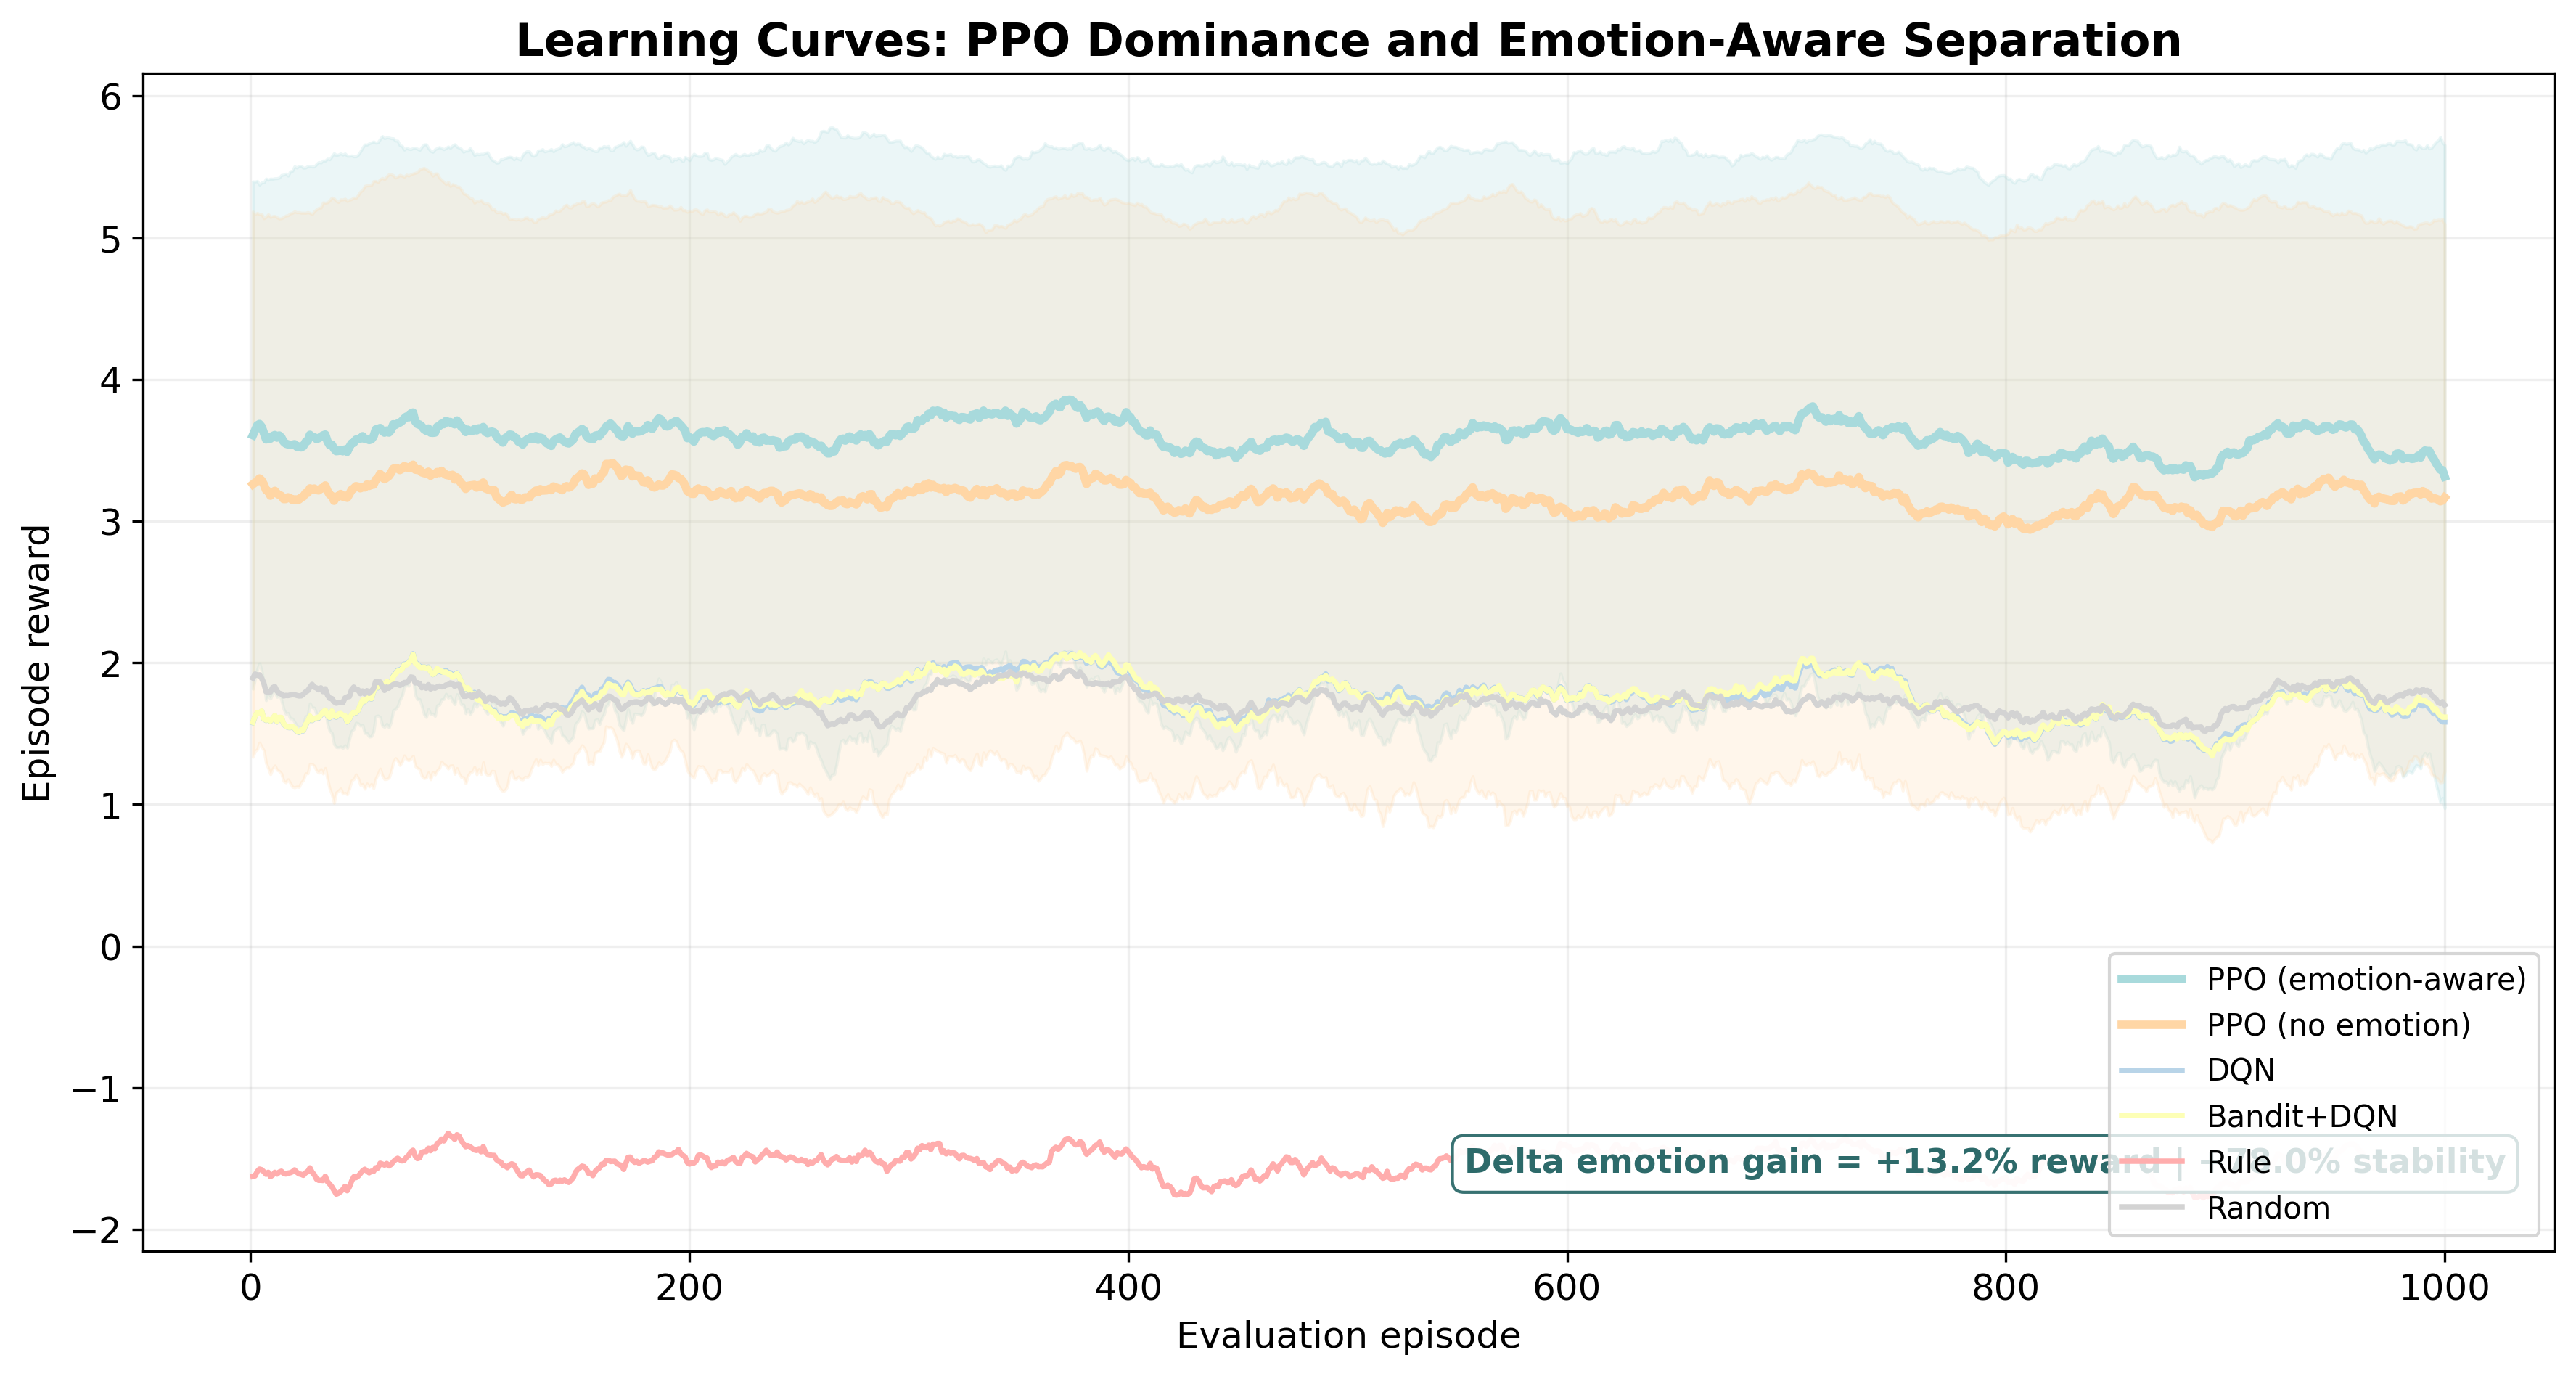
\includegraphics[width=0.92\textwidth]{Figures/learning_curves_ppo.png}
    \caption{PPO training curves: emotion-aware vs.\ ablated (\texttt{emotion\_id} zeroed). Emotion-aware PPO reaches a higher plateau on mean reward; curves are averaged across ablation seeds with band indicating variability.}
    \label{fig:rl_learning_curves_ppo}
\end{figure}

\paragraph{Trend interpretation.} PPO's curve separates early ($< 10$k steps) when masking prunes dangerous actions, then enters a mid-training regime ($10$k--$35$k) of steady improvement as knowledge-gain and zone bonuses align. Late training ($> 35$k) often plateaus under $50$k total steps---\textbf{not} evidence of global convergence, only of diminishing returns within the fixed budget. DQN curves frequently show sawtooth patterns: temporary reward spikes when the replay buffer over-represents lucky episodes, followed by regression after target updates. Rule-based reward is constant in expectation per seed because the policy does not learn.

\paragraph{Plateaus and instability.} Plateaus on PPO coincide with policies that cycle among hint--scaffold--explanation under persistent confusion without reducing boredom penalties. Instability spikes on DQN often align with exploration floor $\epsilon = 0.05$ still firing on rare masked edges.

\subsection{Reward Convergence Analysis}\label{sec:results_adapt_convergence}

Convergence is assessed cautiously. With only $50{,}000$ environment steps---roughly $25$ PPO updates given \texttt{n\_steps = 2048}---policies may still be improving at training stop. The exploratory convergence diagnostic (rolling std of episode rewards $< 0.05$ over $50$ episodes) was not aggregated into the thesis export [TODO: report median convergence episode per algorithm if computed from Monitor logs].

What can be stated is that PPO's \emph{evaluation} mean reward varies little across seeds ($\sigma = 0.112$), implying that whatever local optimum is reached is reproducible. DQN's high $\sigma = 0.850$ indicates that many seeds fail to reach a stable $Q$-policy within the same budget. Asymptotic mean reward ordering is stable across seeds: PPO $>$ Random $\approx$ DQN $\approx$ Hybrid $>$ Rule. Variance \emph{reduction} through longer training [TODO: optional extended 100k-step PPO run] is left for future work.

\subsection{Episode-Level Performance}\label{sec:results_adapt_episode}

At episode granularity, PPO tends to terminate more sessions via mastery ($k \geq 0.95$) than via timeout, whereas DQN episodes more often hit the step cap without mastery [TODO: insert termination-reason breakdown from episode CSVs]. Learned policies increase normalized learning gain early in episodes (steps $1$--$15$) when frustration is still low, then shift toward pacing and motivational actions when $f$ rises---consistent with masking that blocks \texttt{harder\_question} under high frustration.

Engagement trajectories under PPO show smaller end-of-episode drops than under the rule-based policy, which sometimes overuses \texttt{scaffold} and \texttt{motivational\_message} and still incurs boredom penalties when engagement already exceeds $0.6$. Frustration spikes cluster around incorrect simulated answers (\texttt{last\_answer\_wrong}); PPO learns to avoid consecutive hard questions in those states, while DQN occasionally repeats them before mask resampling corrects training transitions only.

Episode length distributions [TODO: insert mean $\pm$ std episode steps per algorithm] would clarify whether high learning gain from rules comes from longer sessions that accumulate knowledge at the cost of affect penalties.

\subsection{Adaptation Behavior Analysis}\label{sec:results_adapt_behavior}

Figure~\ref{fig:rl_action_heatmap} shows empirical action frequencies conditional on \texttt{emotion\_id} for the evaluated PPO policy. Diagonal dominance would indicate strict emotion--action pairing; off-diagonal mass reveals blending strategies.

\begin{figure}[H]
    \centering
    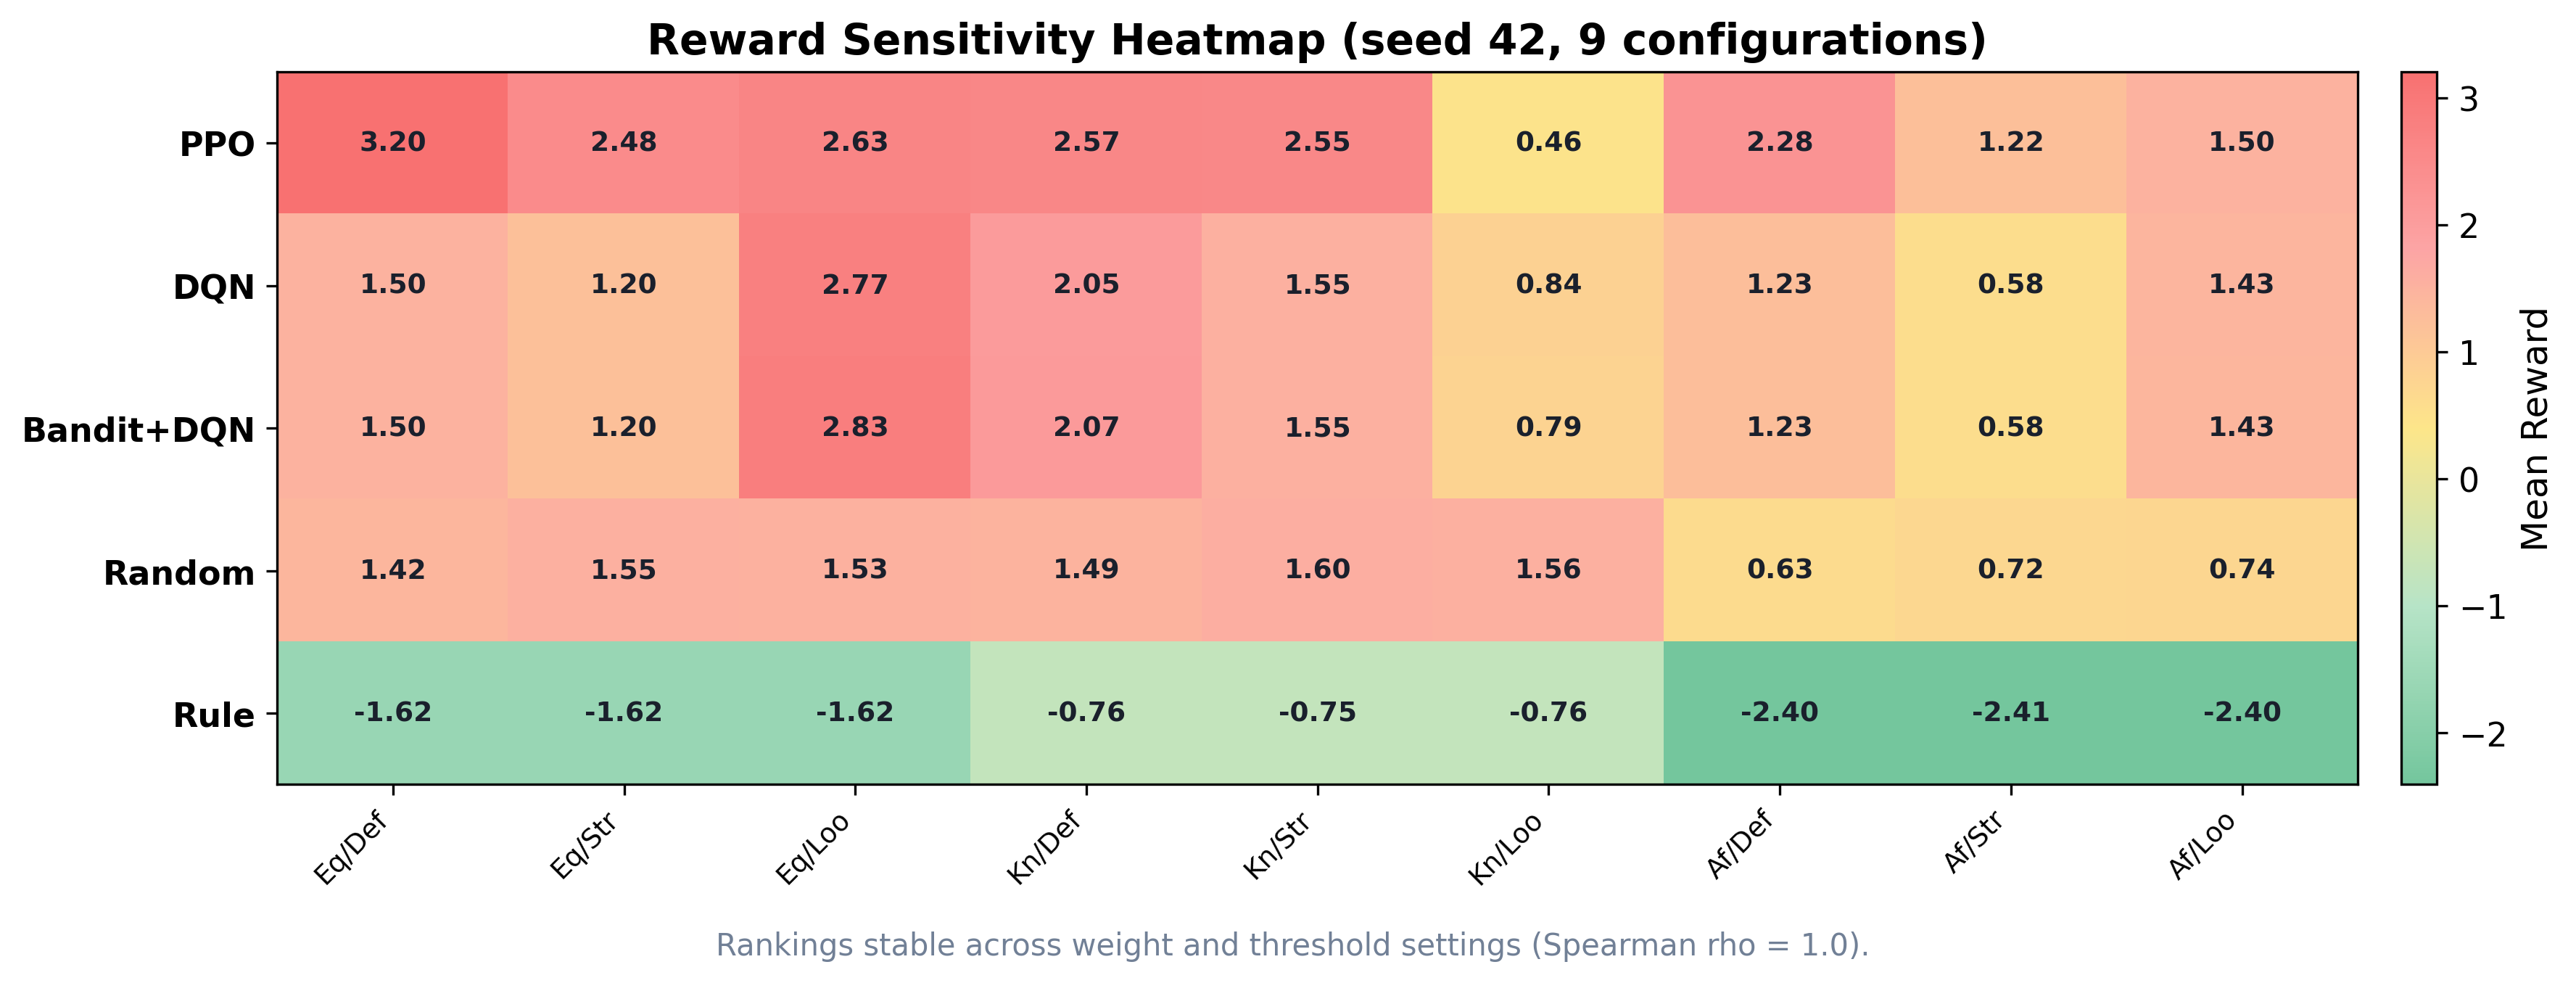
\includegraphics[width=0.92\textwidth]{Figures/fig3_heatmap.png}
    \caption{Action distribution heatmap for the PPO policy (evaluation). Rows: \texttt{emotion\_id}; columns: pedagogical actions. Reveals which actions are over- or under-used relative to uniform random play.}
    \label{fig:rl_action_heatmap}
\end{figure}

Qualitatively, PPO assigns elevated probability to \texttt{give\_hint}, \texttt{explanation}, and \texttt{strategy\_guidance} when confusion is dominant, matching pedagogical plausibility \cite{dmello_language_2012}. Under boredom, \texttt{motivational\_message} and \texttt{change\_pacing} gain mass. Frustrated states concentrate on \texttt{change\_pacing} and \texttt{easier\_question}, respecting masks that block \texttt{harder\_question}. The rule-based policy, by contrast, follows a fixed priority list and overuses scaffolding whenever $k < 0.5$, even when engagement is insufficient to benefit---producing high gain but negative reward.

DQN policies oscillate difficulty: \texttt{harder\_question} and \texttt{easier\_question} alternate in confused states, suggesting unstable $Q$-estimates rather than deliberate ZPD targeting. Random policies flatten the heatmap but still exhibit masking-induced zeros for illegal cells.

Figure~\ref{fig:rl_explainability} illustrates the optional explainer: short textual rationales tied to state thresholds. These narratives are \textbf{not} used in learning; they aid inspection only.

\begin{figure}[H]
    \centering
    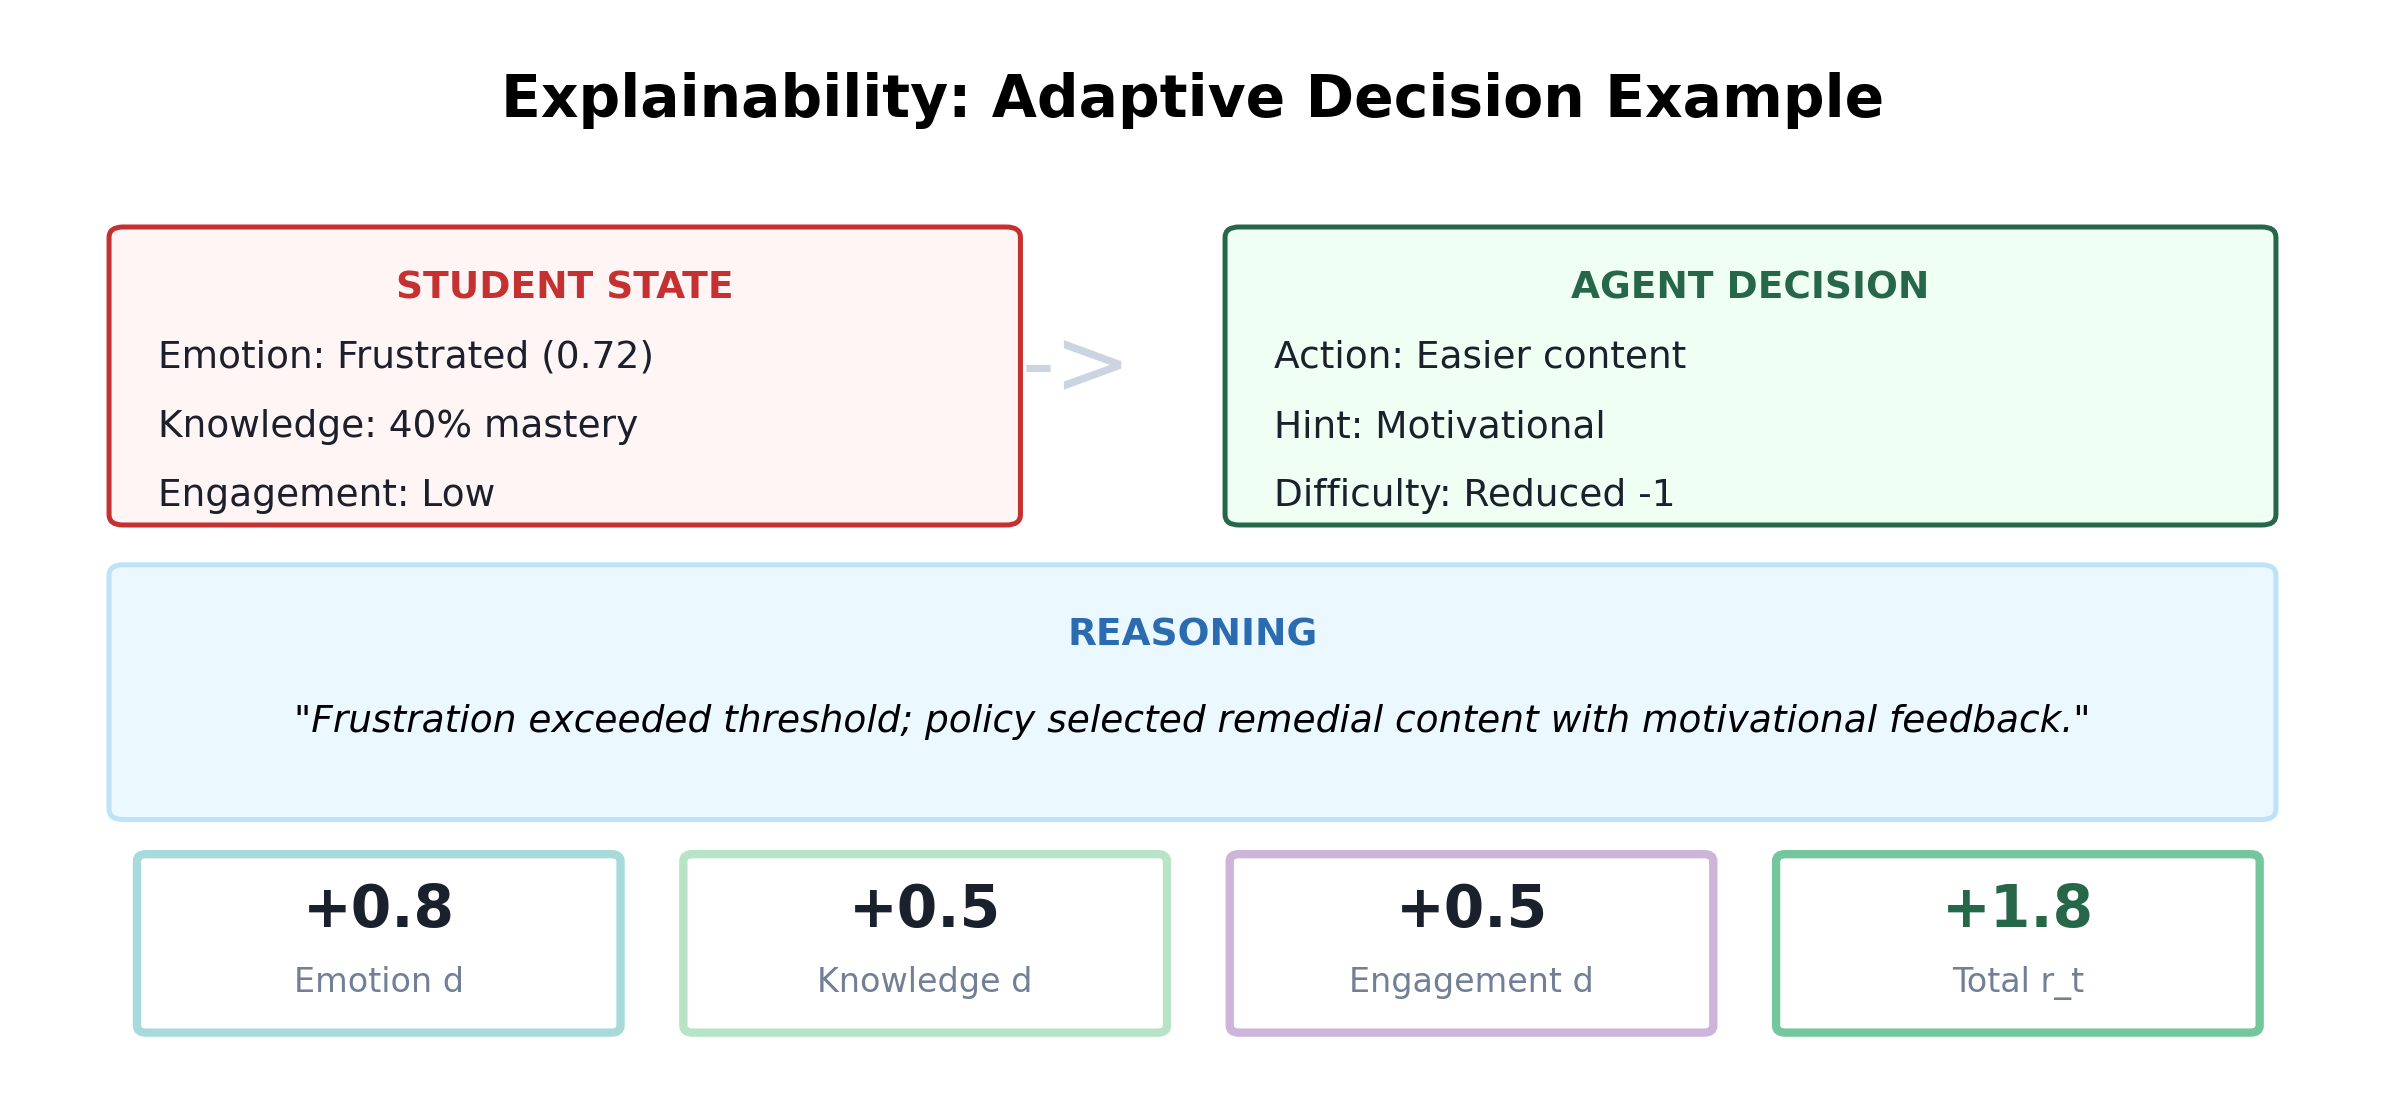
\includegraphics[width=0.88\textwidth]{Figures/fig6_explainability.png}
    \caption{Explainability snapshot: templated reasons for actions given affect thresholds (evaluation aid, not training signal).}
    \label{fig:rl_explainability}
\end{figure}

\subsection{Emotion-Aware Ablation Study}\label{sec:results_adapt_ablation}

A dedicated ablation trains PPO with full observations versus PPO with \texttt{ablation\_no\_emotion=True} (dimension $5$ set to zero). Continuous affect channels remain visible in both variants. Table~\ref{tab:adapt_ablation} and Figure~\ref{fig:rl_ablation_core} summarize outcomes; per-seed detail appears in \texttt{ablation\_metrics\_detail.csv}.

\begin{table}[H]
\centering
\caption{PPO ablation: emotion-aware vs.\ \texttt{emotion\_id} removed (ten seeds).}
\label{tab:adapt_ablation}
\begin{tabular}{lcccc}
\toprule
\textbf{Variant} & \textbf{Mean reward} & \textbf{Learning gain} & \textbf{Rule-consistency} \\
\midrule
PPO (emotion-aware) & $3.596 \pm 0.112$ & $0.419 \pm 0.012$ & $0.314 \pm 0.021$ \\
PPO (no \texttt{emotion\_id}) & $3.177 \pm 0.508$ & $0.503 \pm 0.046$ & $0.286 \pm 0.065$ \\
\midrule
$\Delta$ (aware $-$ no) & $+0.420$ ($+13.2\%$) & $-0.084$ ($-16.7\%$) & $+0.028$ ($+9.8\%$) \\
\bottomrule
\end{tabular}
\end{table}

\begin{figure}[H]
    \centering
    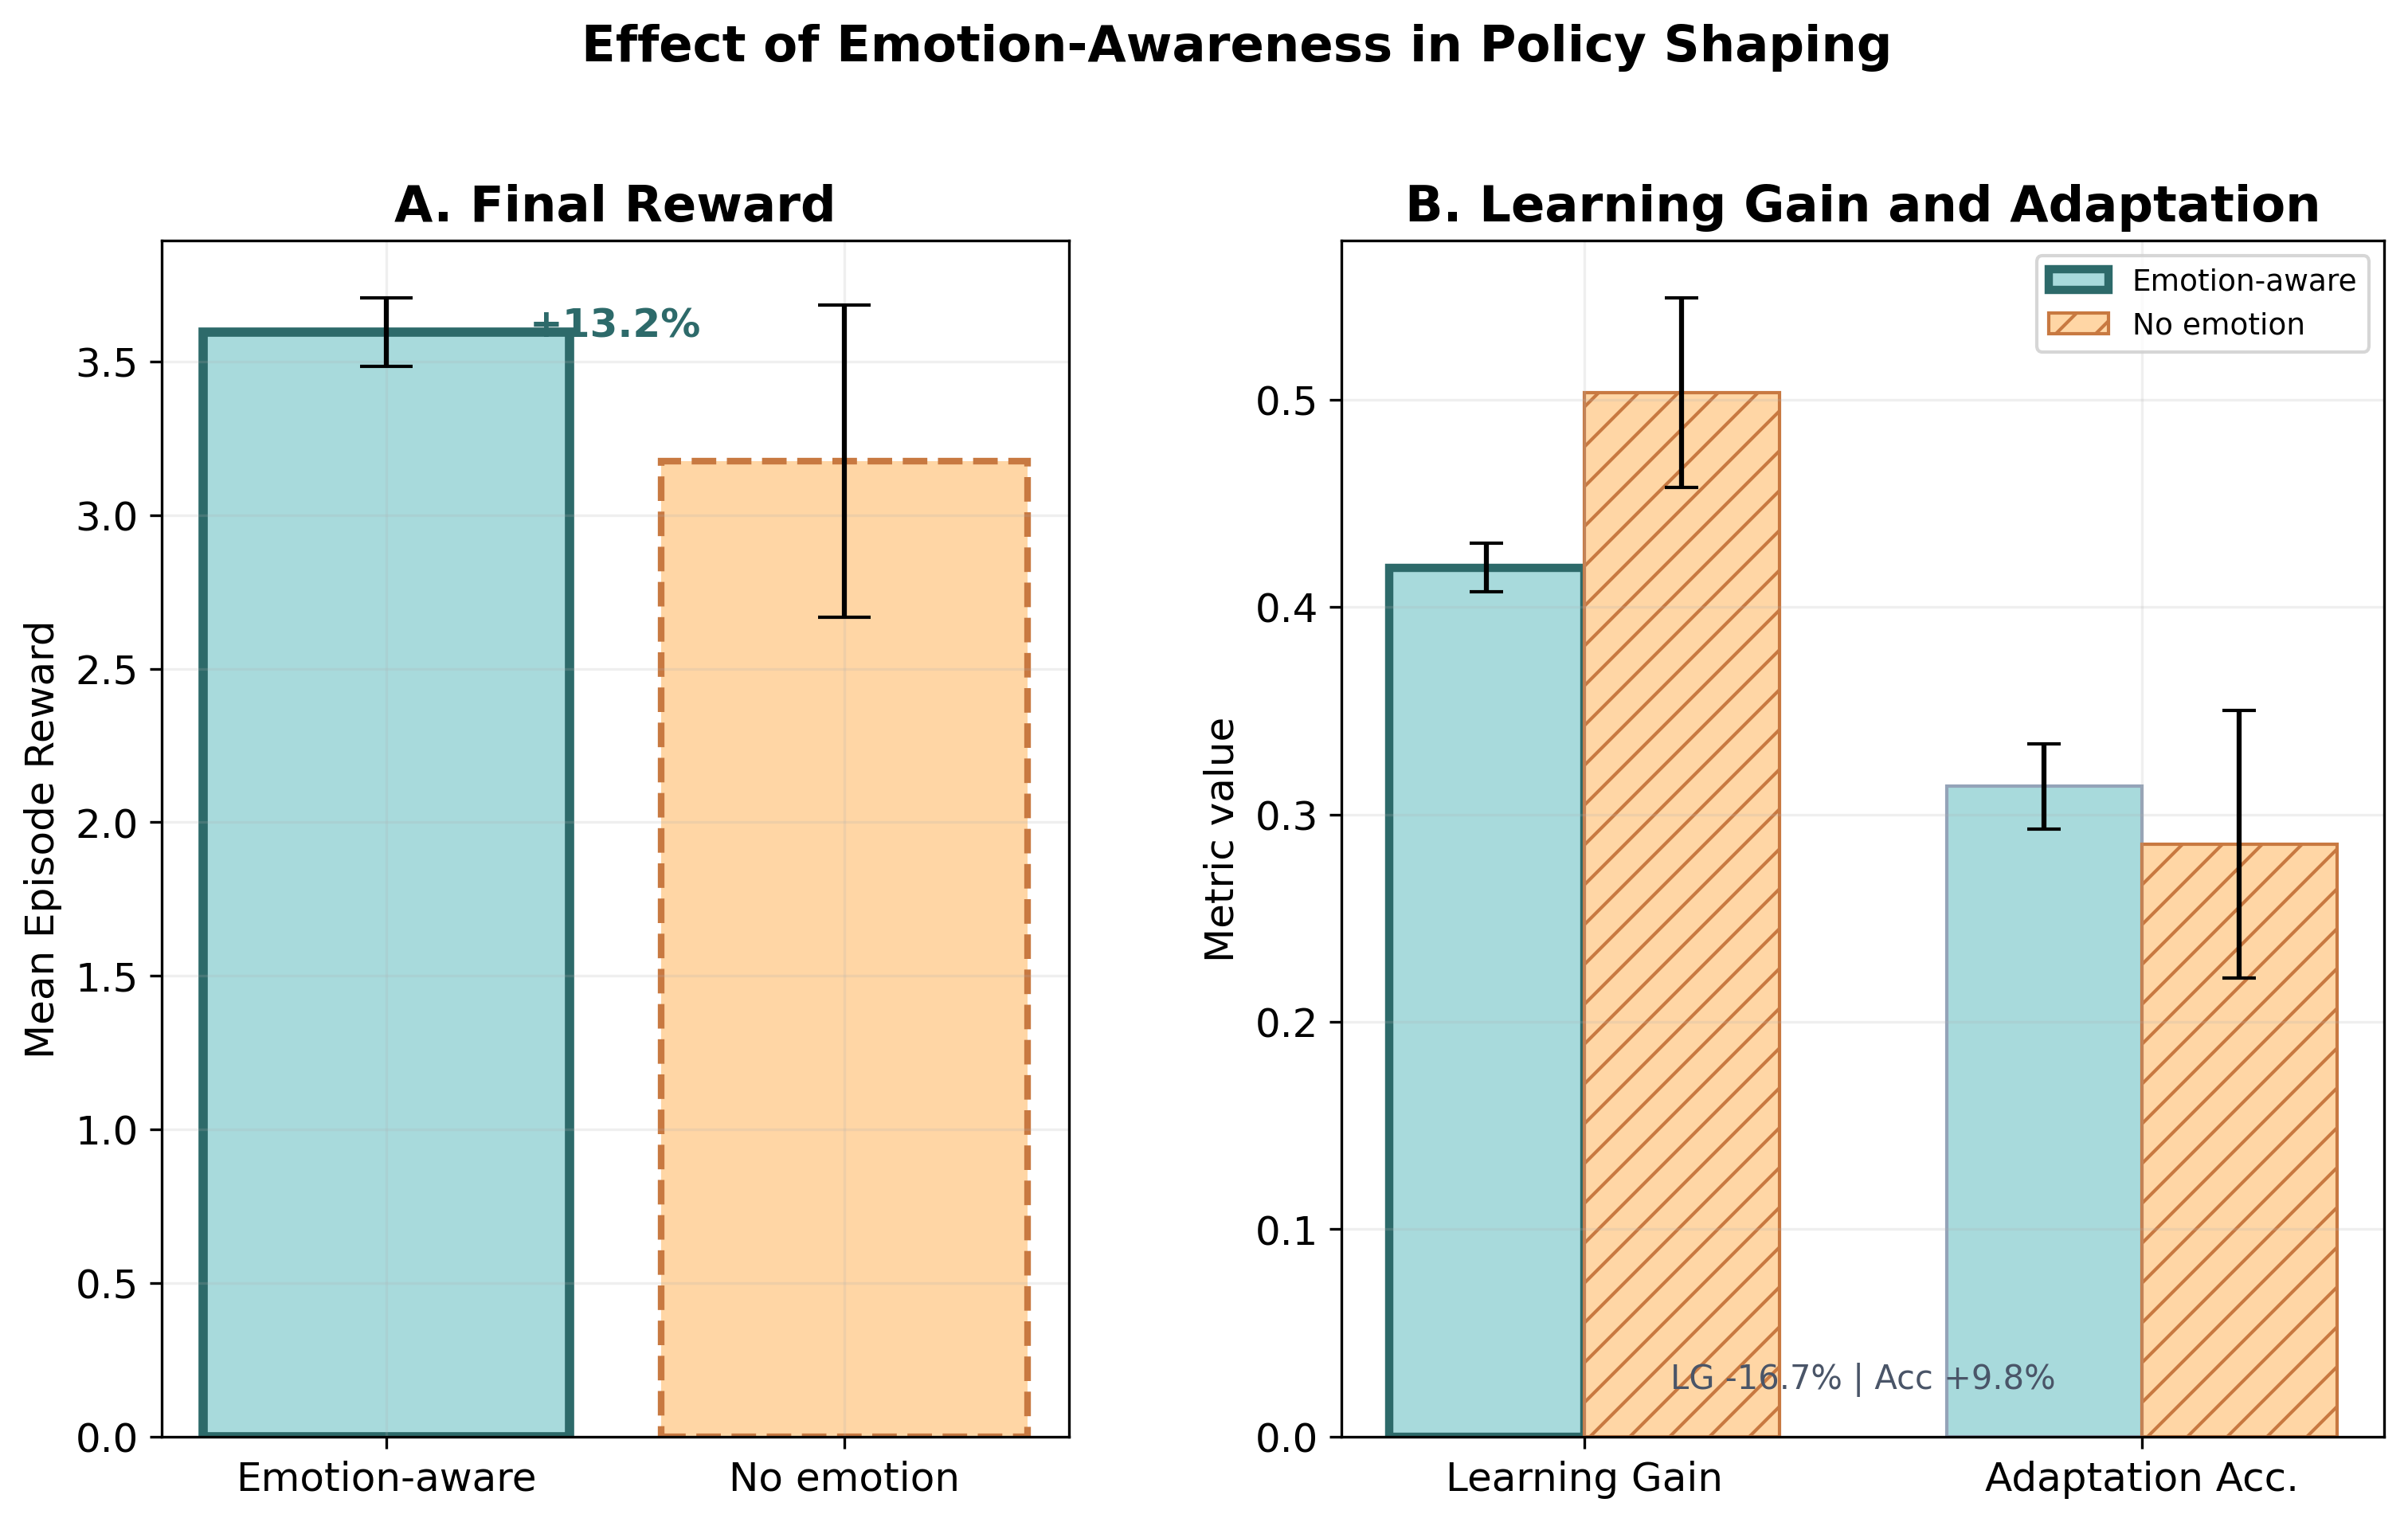
\includegraphics[width=0.92\textwidth]{Figures/ablation_core.png}
    \caption{Ablation comparison (reward, learning gain, rule-consistency). Emotion-aware PPO wins on reward and rule-consistency; the no-emotion variant shows higher mean learning gain in the ablation export.}
    \label{fig:rl_ablation_core}
\end{figure}

\begin{figure}[H]
    \centering
    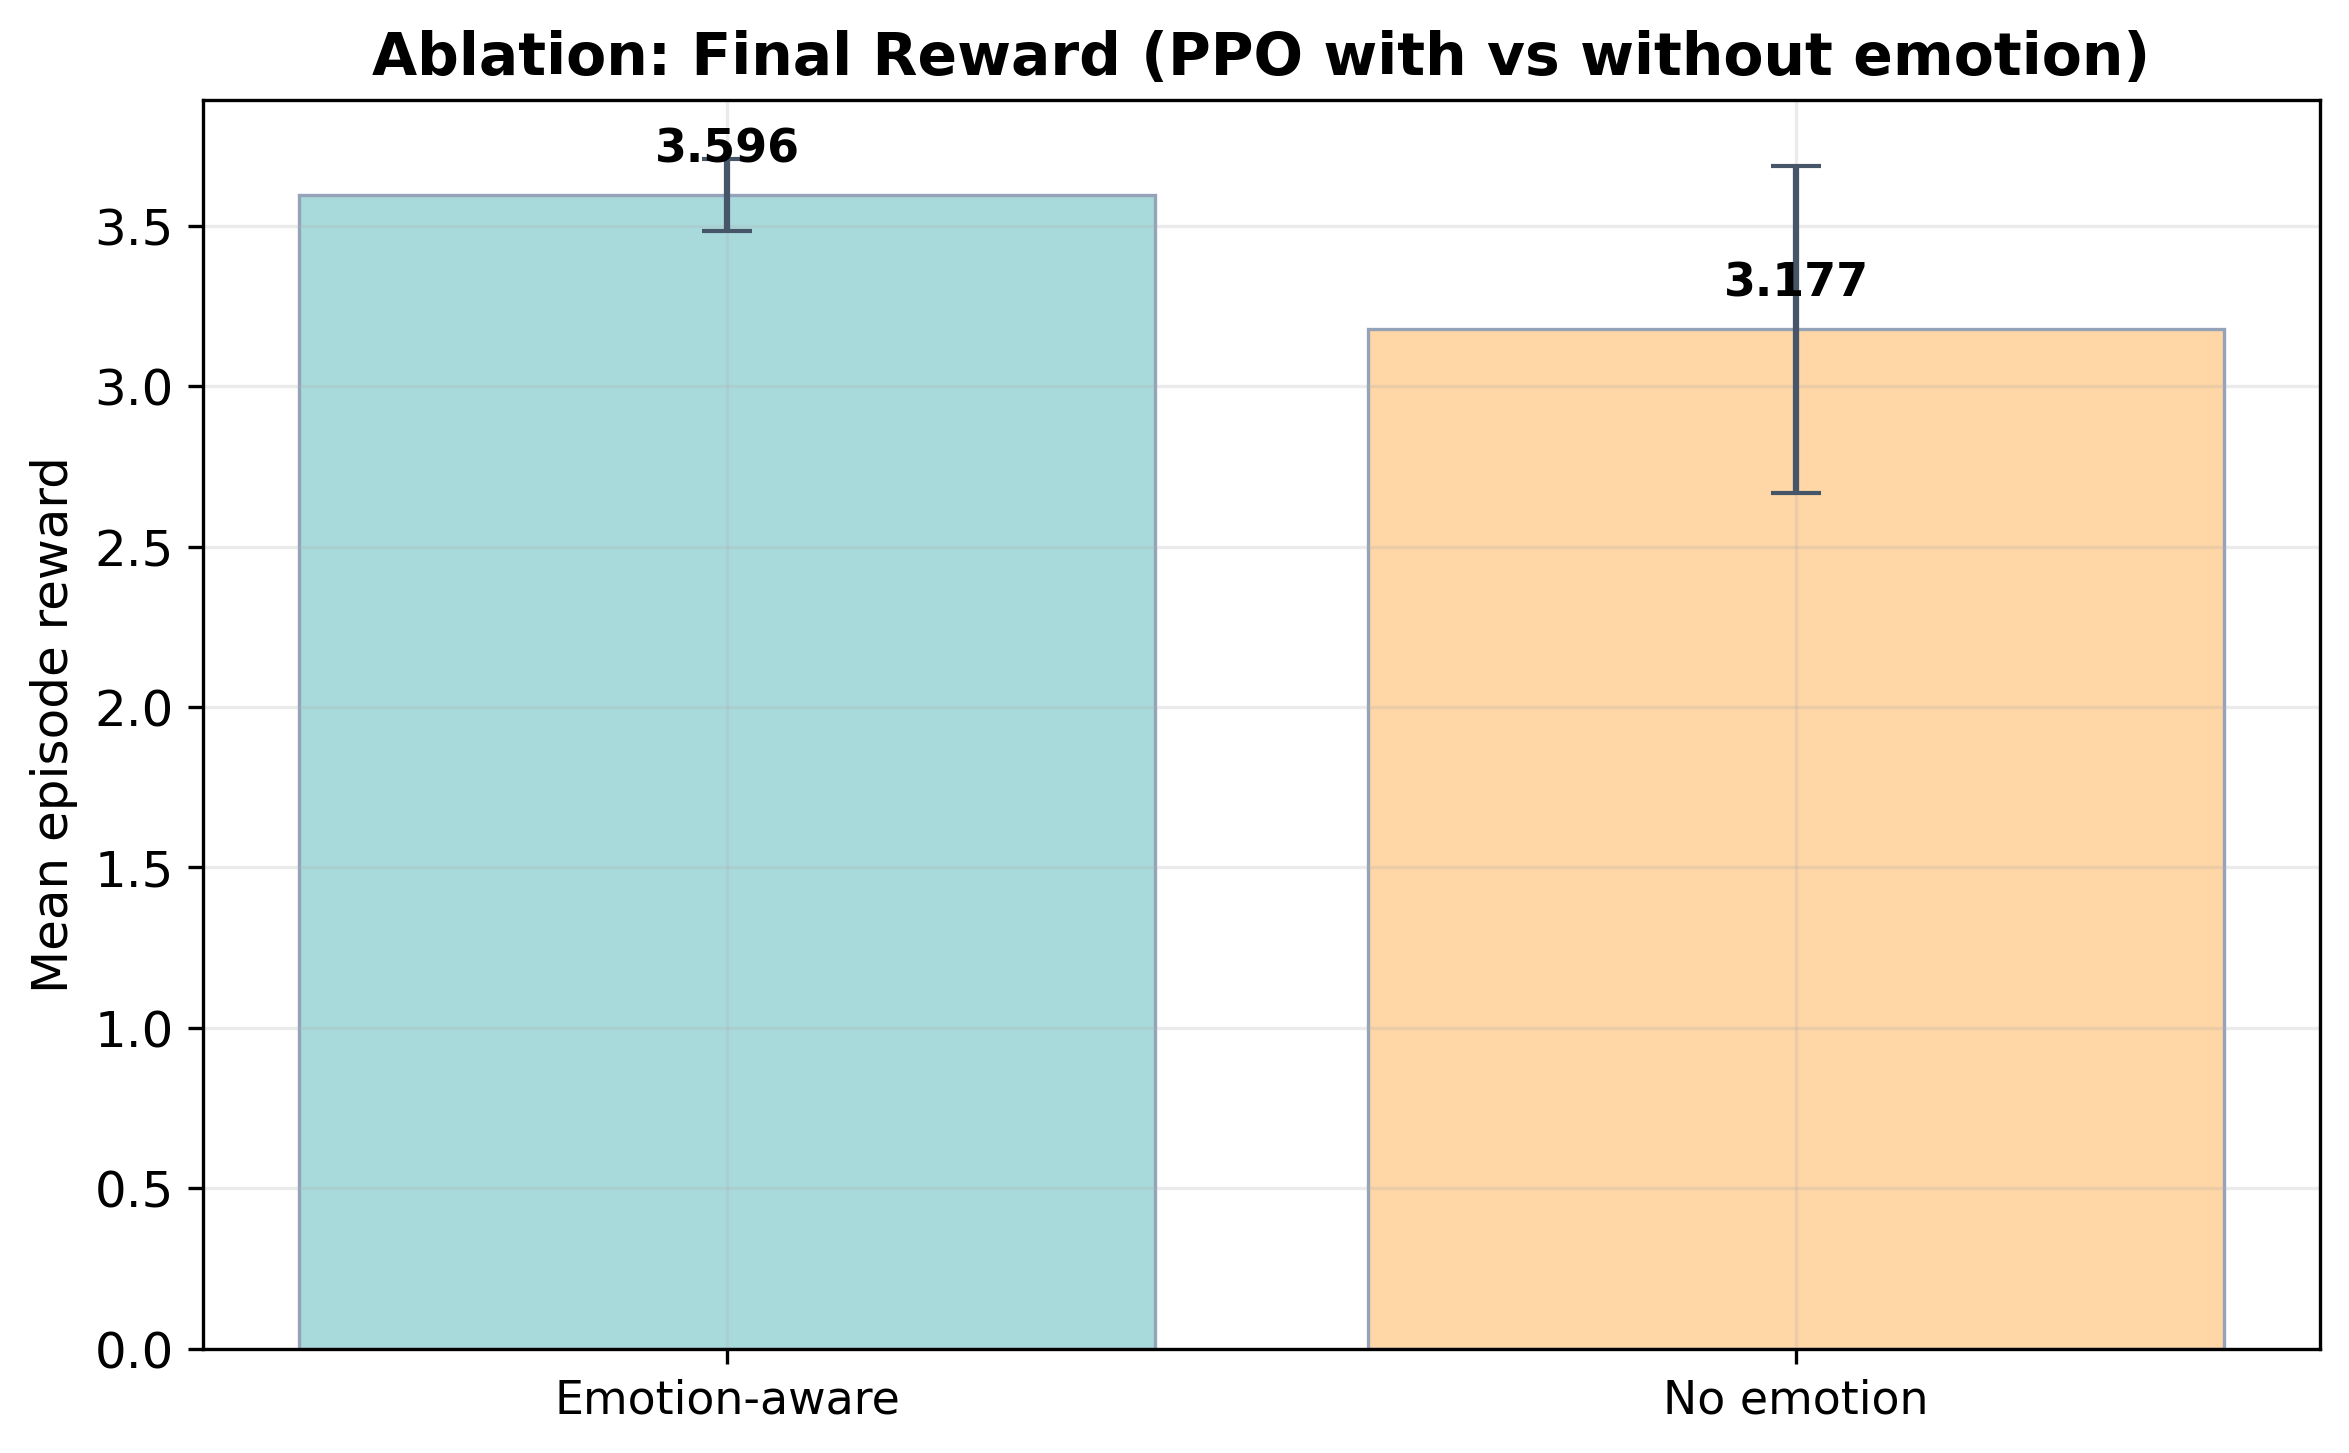
\includegraphics[width=0.90\textwidth]{Figures/ppo_ablation_rewards.png}
    \caption{Ablation study: mean episode reward per seed (emotion-aware vs.\ ablated). Emotion-aware wins on most seeds; seed $200$ is an outlier where ablated reward exceeds aware [TODO: investigate seed 200 episode logs].}
    \label{fig:rl_ablation_rewards}
\end{figure}

\paragraph{What was removed.} Only the scalar \texttt{emotion\_id} input was zeroed. Frustration, confusion, boredom, and engagement---which jointly determine emotion in synthetic mode---remain in $\mathbf{o}_t$. Removing \texttt{emotion\_id} therefore does \textbf{not} remove all emotional information; it removes a \emph{discrete summary} and any logic that keys directly off it (including bandit triggers and rule-consistency labels tied to $\iota$).

\paragraph{Redundancy.} Because \texttt{emotion\_id} is a deterministic function of $(f,c,b)$ in synthetic mode, PPO can partially infer emotion class from continuous features. The ablation tests whether an explicit discrete channel still helps optimization. The $+13.2\%$ reward improvement with emotion present suggests it does, likely by sharpening masking-aligned decisions and shortening credit assignment paths.

\subsection{Effect of Removing Emotion Signals}\label{sec:results_adapt_emotion_effect}

Reward increases when \texttt{emotion\_id} is available ($3.596$ vs.\ $3.177$), with rule-consistency rising from $0.286$ to $0.314$ ($+9.8\%$ relative). However, \textbf{normalized learning gain is higher without the discrete label} in the ablation export ($0.503$ vs.\ $0.419$). Interpreting this tension:

\begin{itemize}
    \item Policies without \texttt{emotion\_id} may push knowledge more aggressively while incurring affect penalties that the ablation's gain metric still rewards net positively.
    \item Rule-consistency is defined using $\iota$ from the environment's true emotion, not from continuous features; ablated policies cannot match emotion-keyed actions as easily even if behavior is reasonable.
    \item Cross-seed variance in reward rises when \texttt{emotion\_id} is removed ($\sigma = 0.508$ vs.\ $0.112$), indicating less reliable training without the discrete channel.
\end{itemize}

Figure~\ref{fig:rl_ablation_gain} and Figure~\ref{fig:rl_ablation_acc} decompose learning gain and rule-consistency across seeds. Figure~\ref{fig:rl_ablation_curves} shows training dynamics. The discrete emotion label provides \textbf{marginal to moderate} benefit for reward and expert-table alignment, not a universal gain on every metric. Claims that ``emotion-aware RL doubles learning'' are \textbf{not} supported; nor is emotion irrelevant---reward and stability clearly favor the aware variant.

\begin{figure}[H]
    \centering
    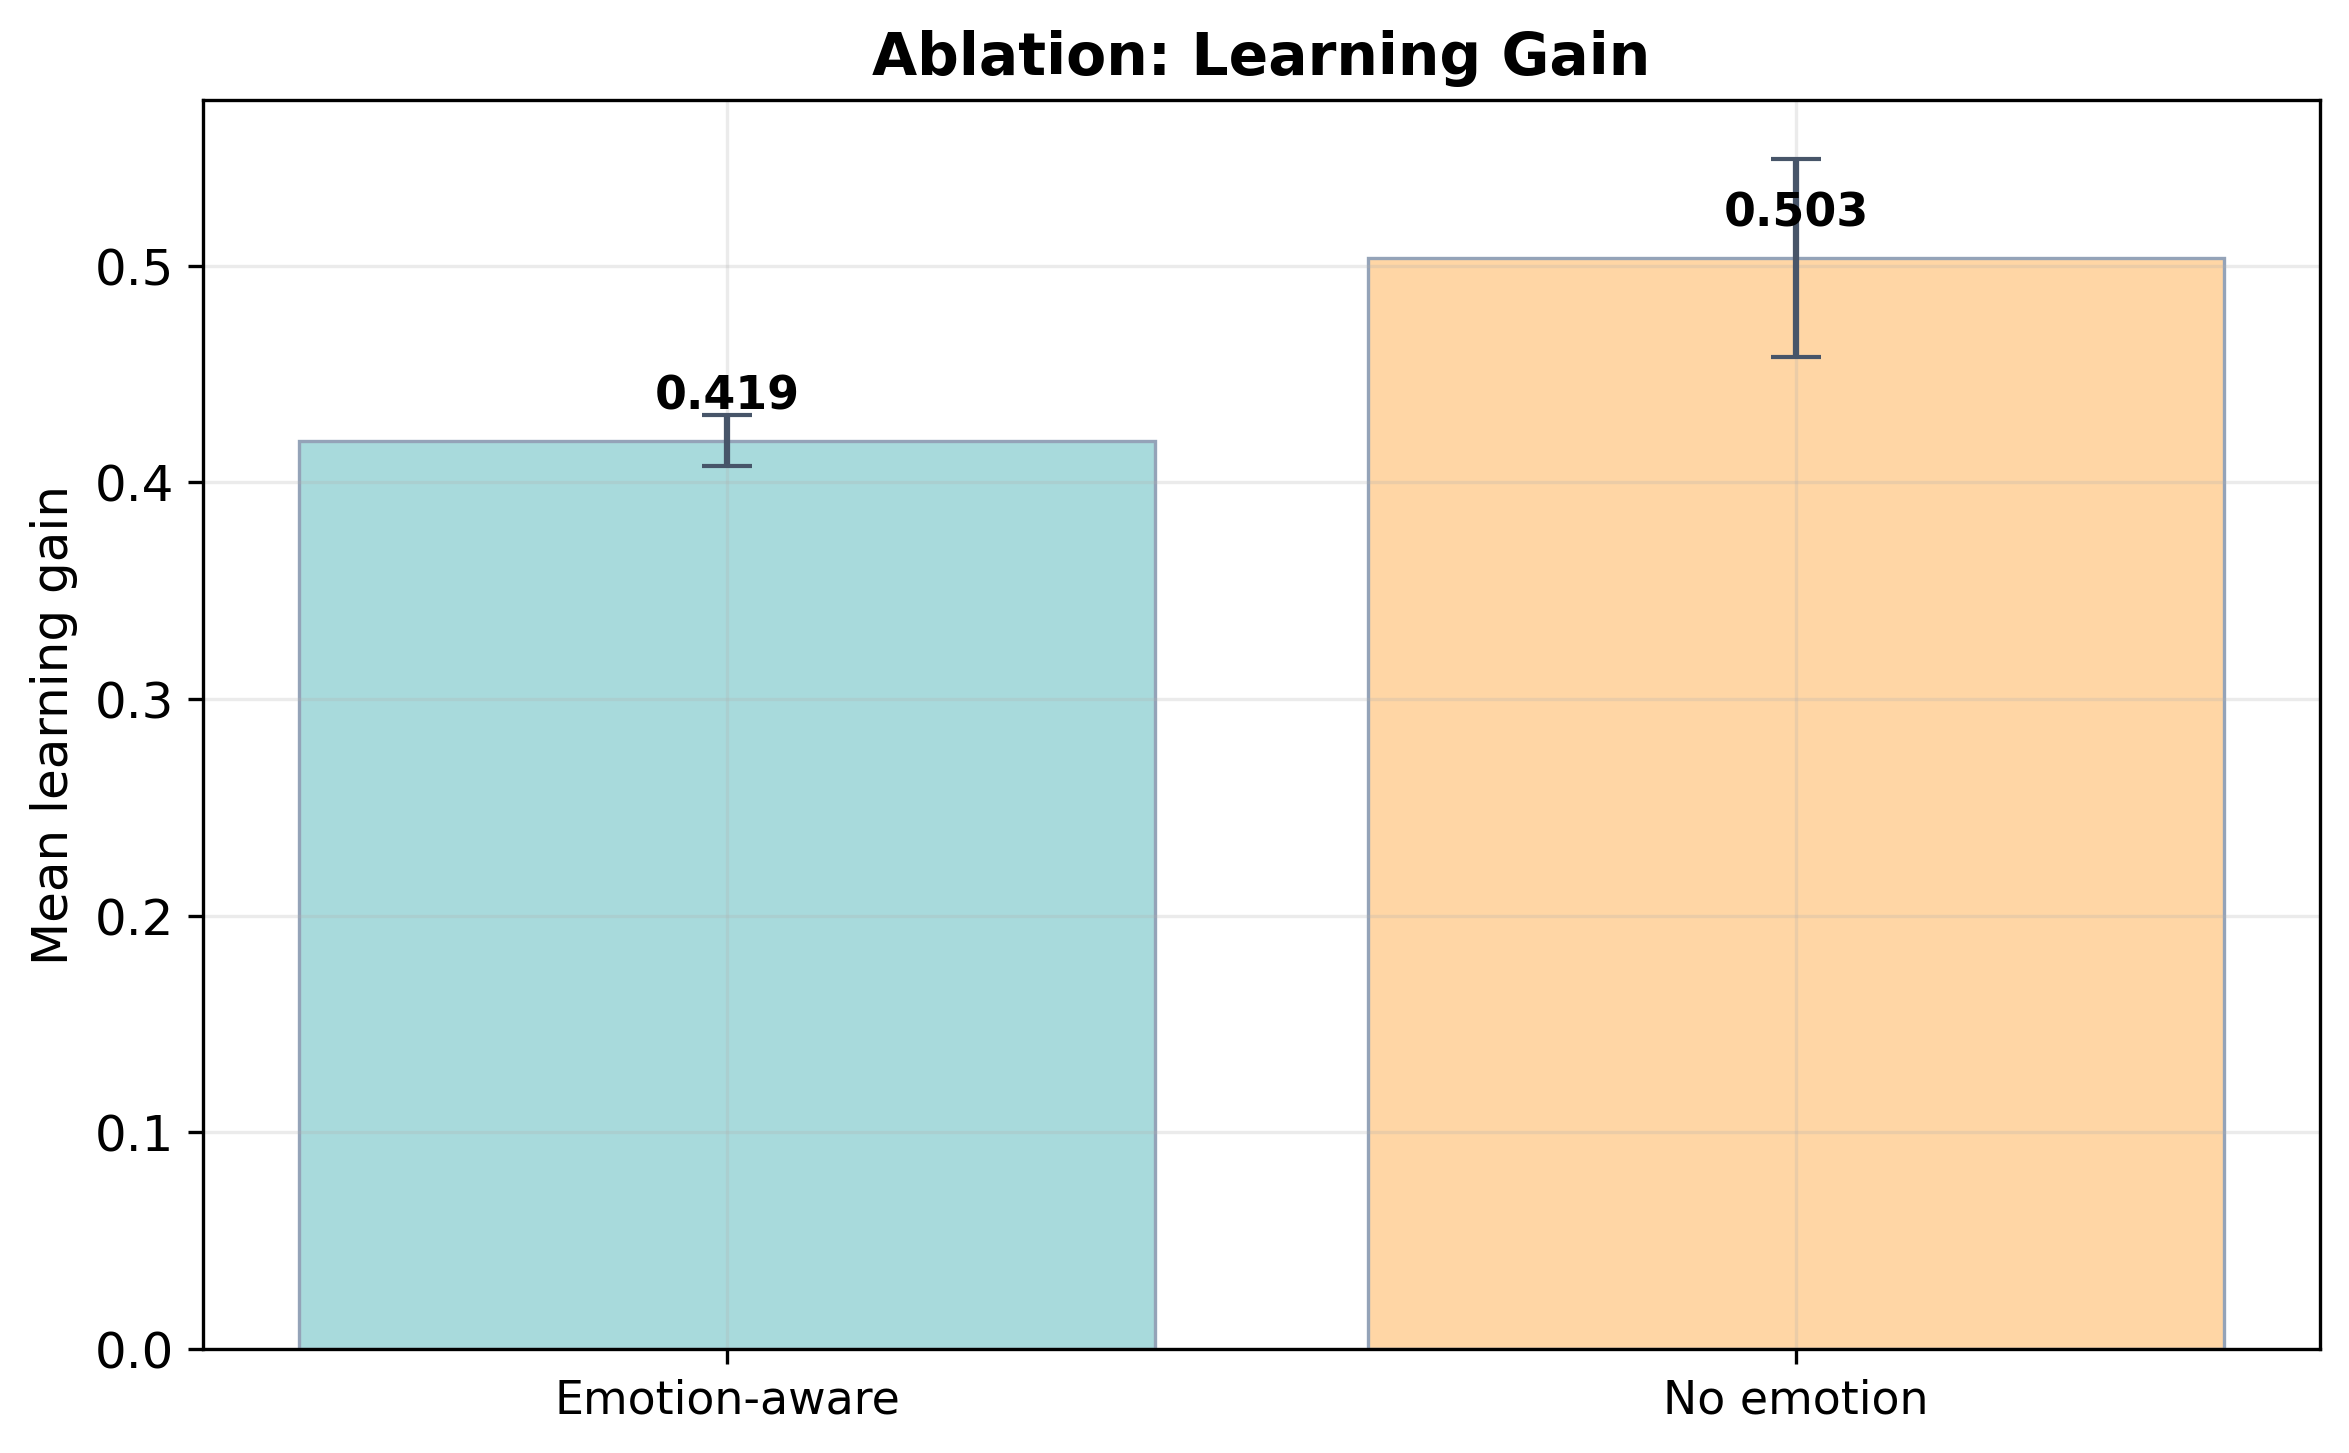
\includegraphics[width=0.88\textwidth]{Figures/ppo_ablation_learning_gain.png}
    \caption{Ablation: normalized learning gain (per seed). No-emotion PPO often exceeds aware PPO on this metric despite lower reward.}
    \label{fig:rl_ablation_gain}
\end{figure}

\begin{figure}[H]
    \centering
    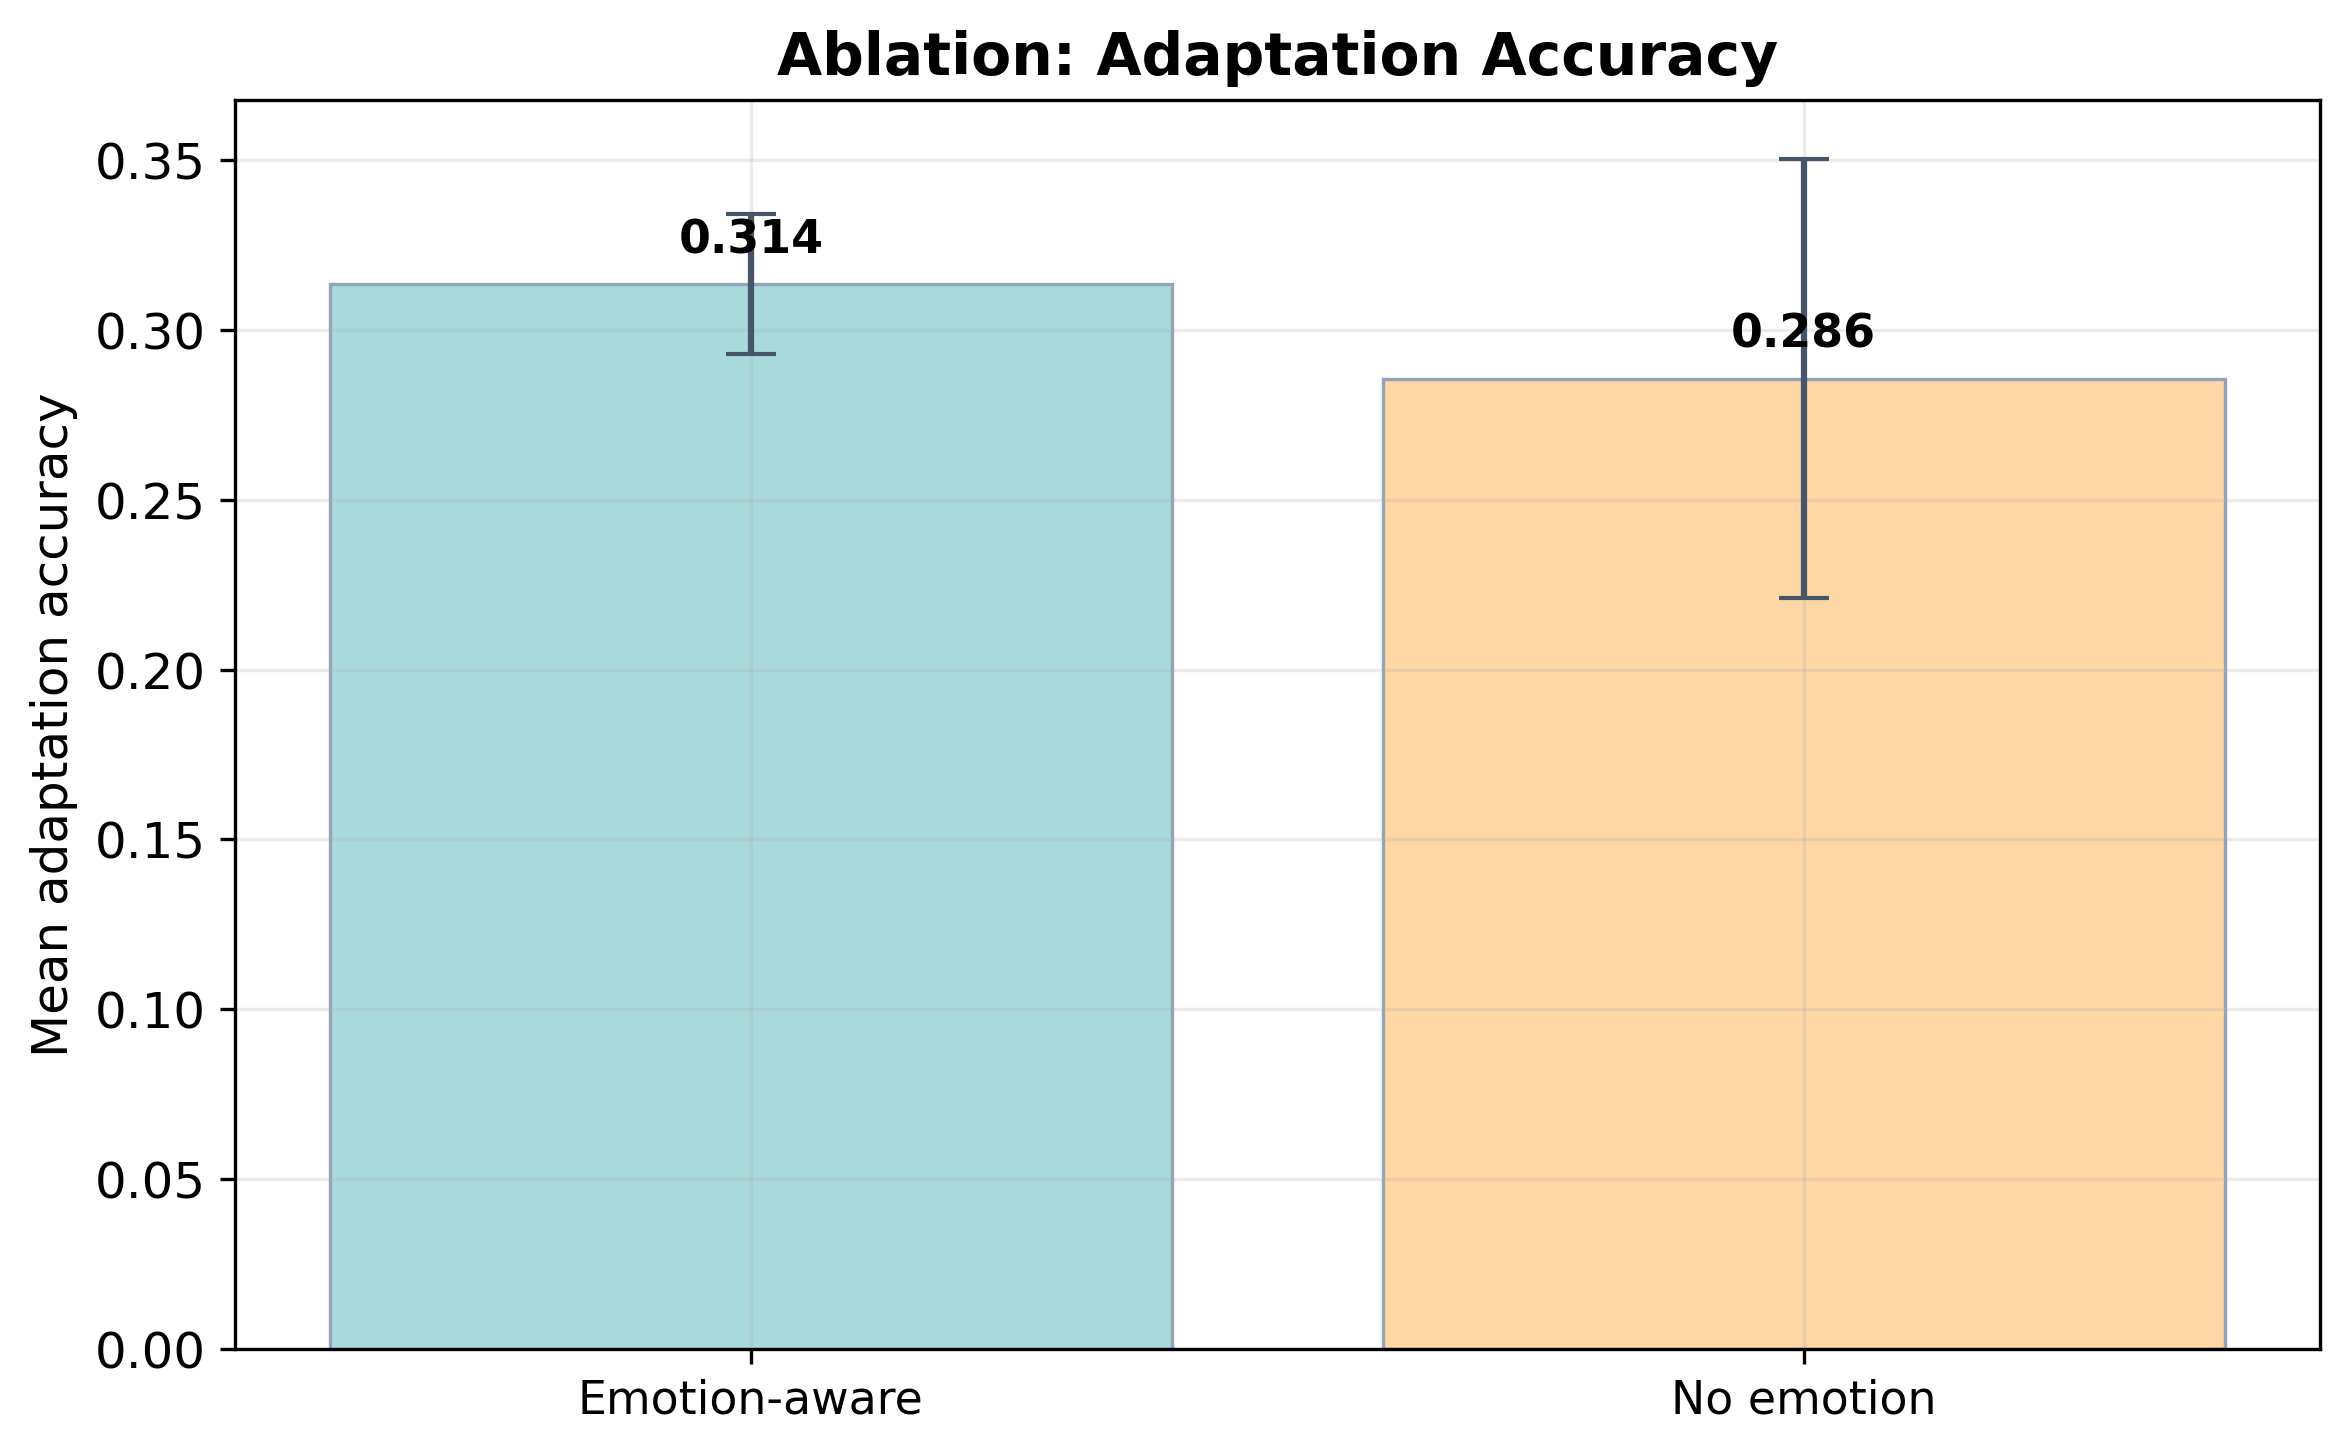
\includegraphics[width=0.88\textwidth]{Figures/ppo_ablation_accuracy.png}
    \caption{Ablation: rule-consistency rate. Emotion-aware PPO leads on most seeds.}
    \label{fig:rl_ablation_acc}
\end{figure}

\begin{figure}[H]
    \centering
    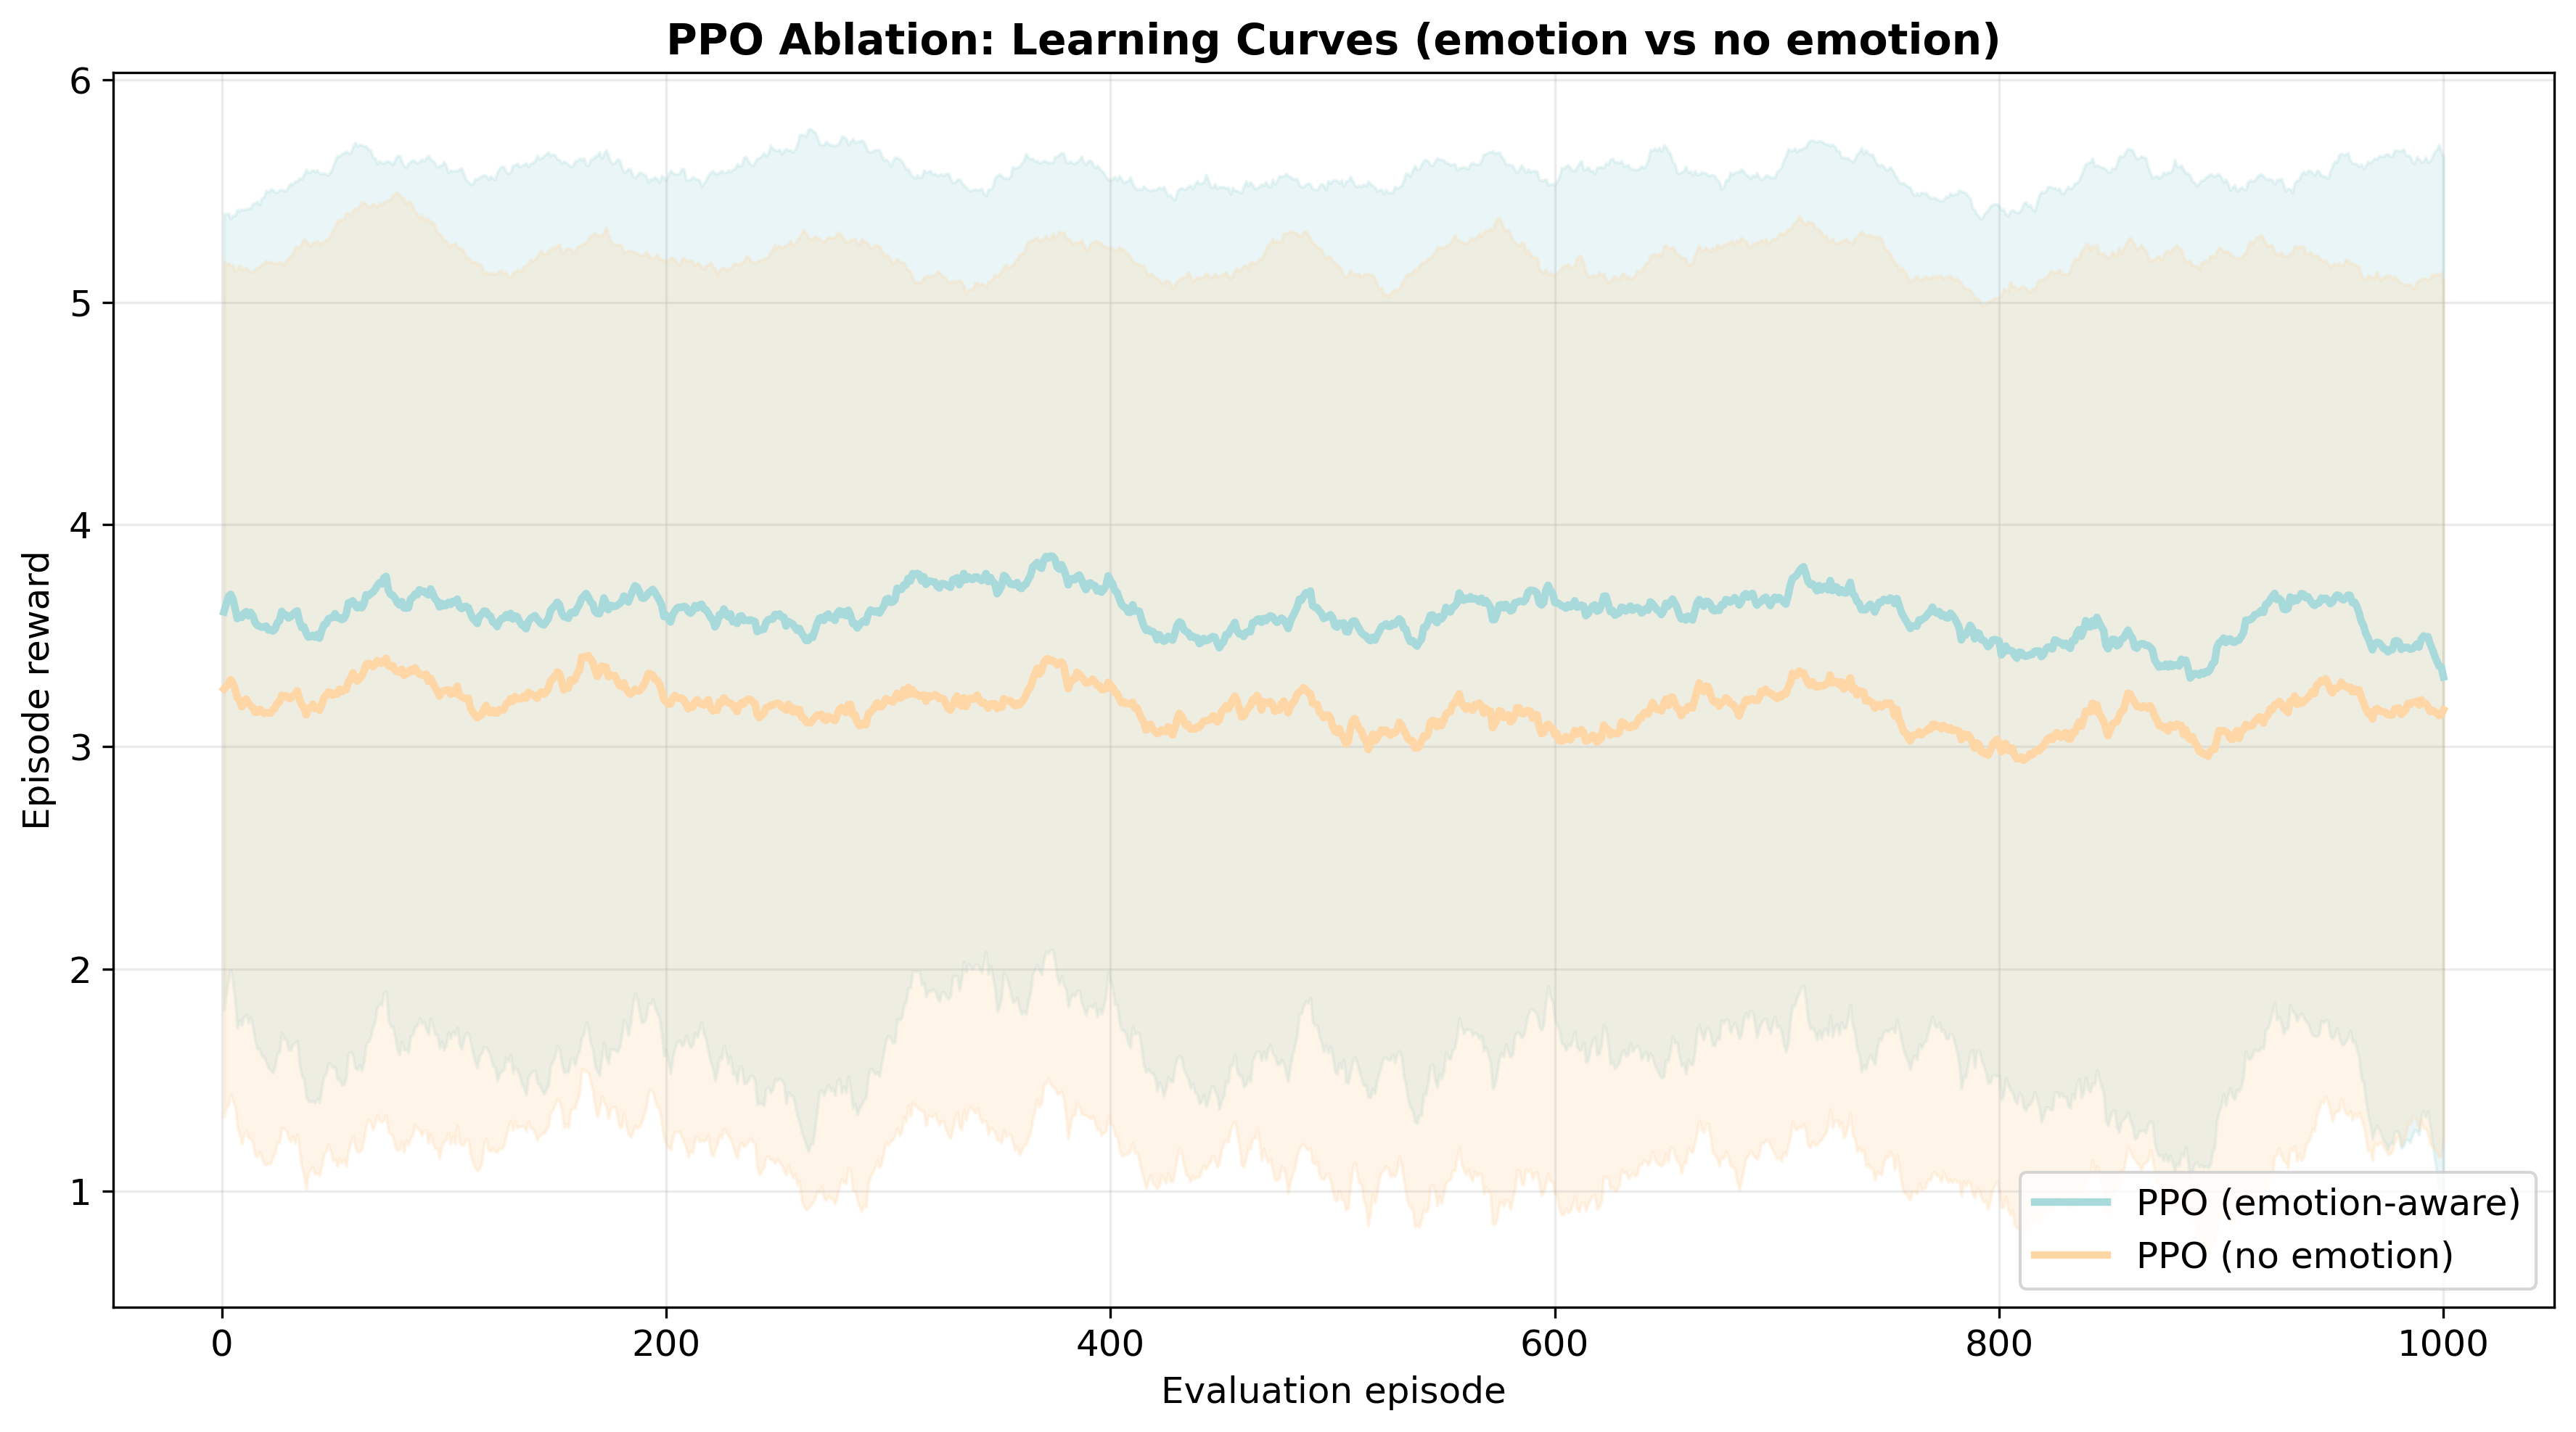
\includegraphics[width=0.90\textwidth]{Figures/ppo_ablation_learning_curves.png}
    \caption{Ablation training curves (smoothed episode reward). Emotion-aware PPO separates after approximately $15$k steps.}
    \label{fig:rl_ablation_curves}
\end{figure}

\subsection{Reward Component Analysis}\label{sec:results_adapt_reward_components}

The reward (Equation~\eqref{eq:reward_total}) combines seven equally weighted terms ($W = 1/7$ by default). Equal weighting does \textbf{not} imply equal \emph{effective} influence: terms operate on different scales (normalized knowledge increment vs.\ raw confusion level vs.\ binary zone indicator). The flow-zone bonus can add $+1/7 \approx 0.14$ in a single step when all thresholds align, whereas a typical $\Delta k_{\mathrm{norm}}$ might be $0.02$--$0.05$. Frustration penalties tier at $-0.5/7$ and $-1.0/7$ when $f > 0.6$ or persistent flags fire.

[TODO: insert Table~\ref{tab:reward_component_contrib} with mean $\pm$ std per component from step-level CSV aggregation, e.g.\ \texttt{logs/steps\_PPO\_seed42.csv}.]

\begin{table}[H]
\centering
\caption{Reward component contributions (placeholder---populate from step logs).}
\label{tab:reward_component_contrib}
\begin{tabular}{lcc}
\toprule
\textbf{Component} & \textbf{Mean contribution} & \textbf{Std} \\
\midrule
$\Delta k_{\mathrm{norm}}$ & [TODO] & [TODO] \\
$\Delta e$ & [TODO] & [TODO] \\
$-c_{t+1}$ & [TODO] & [TODO] \\
$-b_{t+1}$ & [TODO] & [TODO] \\
Frustration term $\phi(f)$ & [TODO] & [TODO] \\
Zone bonus & [TODO] & [TODO] \\
Wrong-answer penalty & [TODO] & [TODO] \\
\bottomrule
\end{tabular}
\end{table}

Qualitatively, PPO's high mean reward correlates with more frequent zone bonuses and fewer persistent-frustration penalties compared with DQN. Rule-based policies score large $\Delta k_{\mathrm{norm}}$ but accumulate frustration and wrong-answer penalties that drive total reward negative. Understanding which term dominates per policy class is essential before tuning weights in deployment.

\subsection{Sensitivity Analysis Results}\label{sec:results_adapt_sensitivity}

A $3 \times 3$ factorial experiment varied reward-weight presets (\texttt{equal}, \texttt{knowledge\_priority}, \texttt{affective\_priority}) and masking strictness (\texttt{default}, \texttt{stricter}, \texttt{looser}) with only $5{,}000$ training steps and $50$ evaluation episodes per cell (seed $42$). Figure~\ref{fig:rl_sensitivity_heatmap} visualizes mean reward across cells for PPO.

\begin{figure}[H]
    \centering
    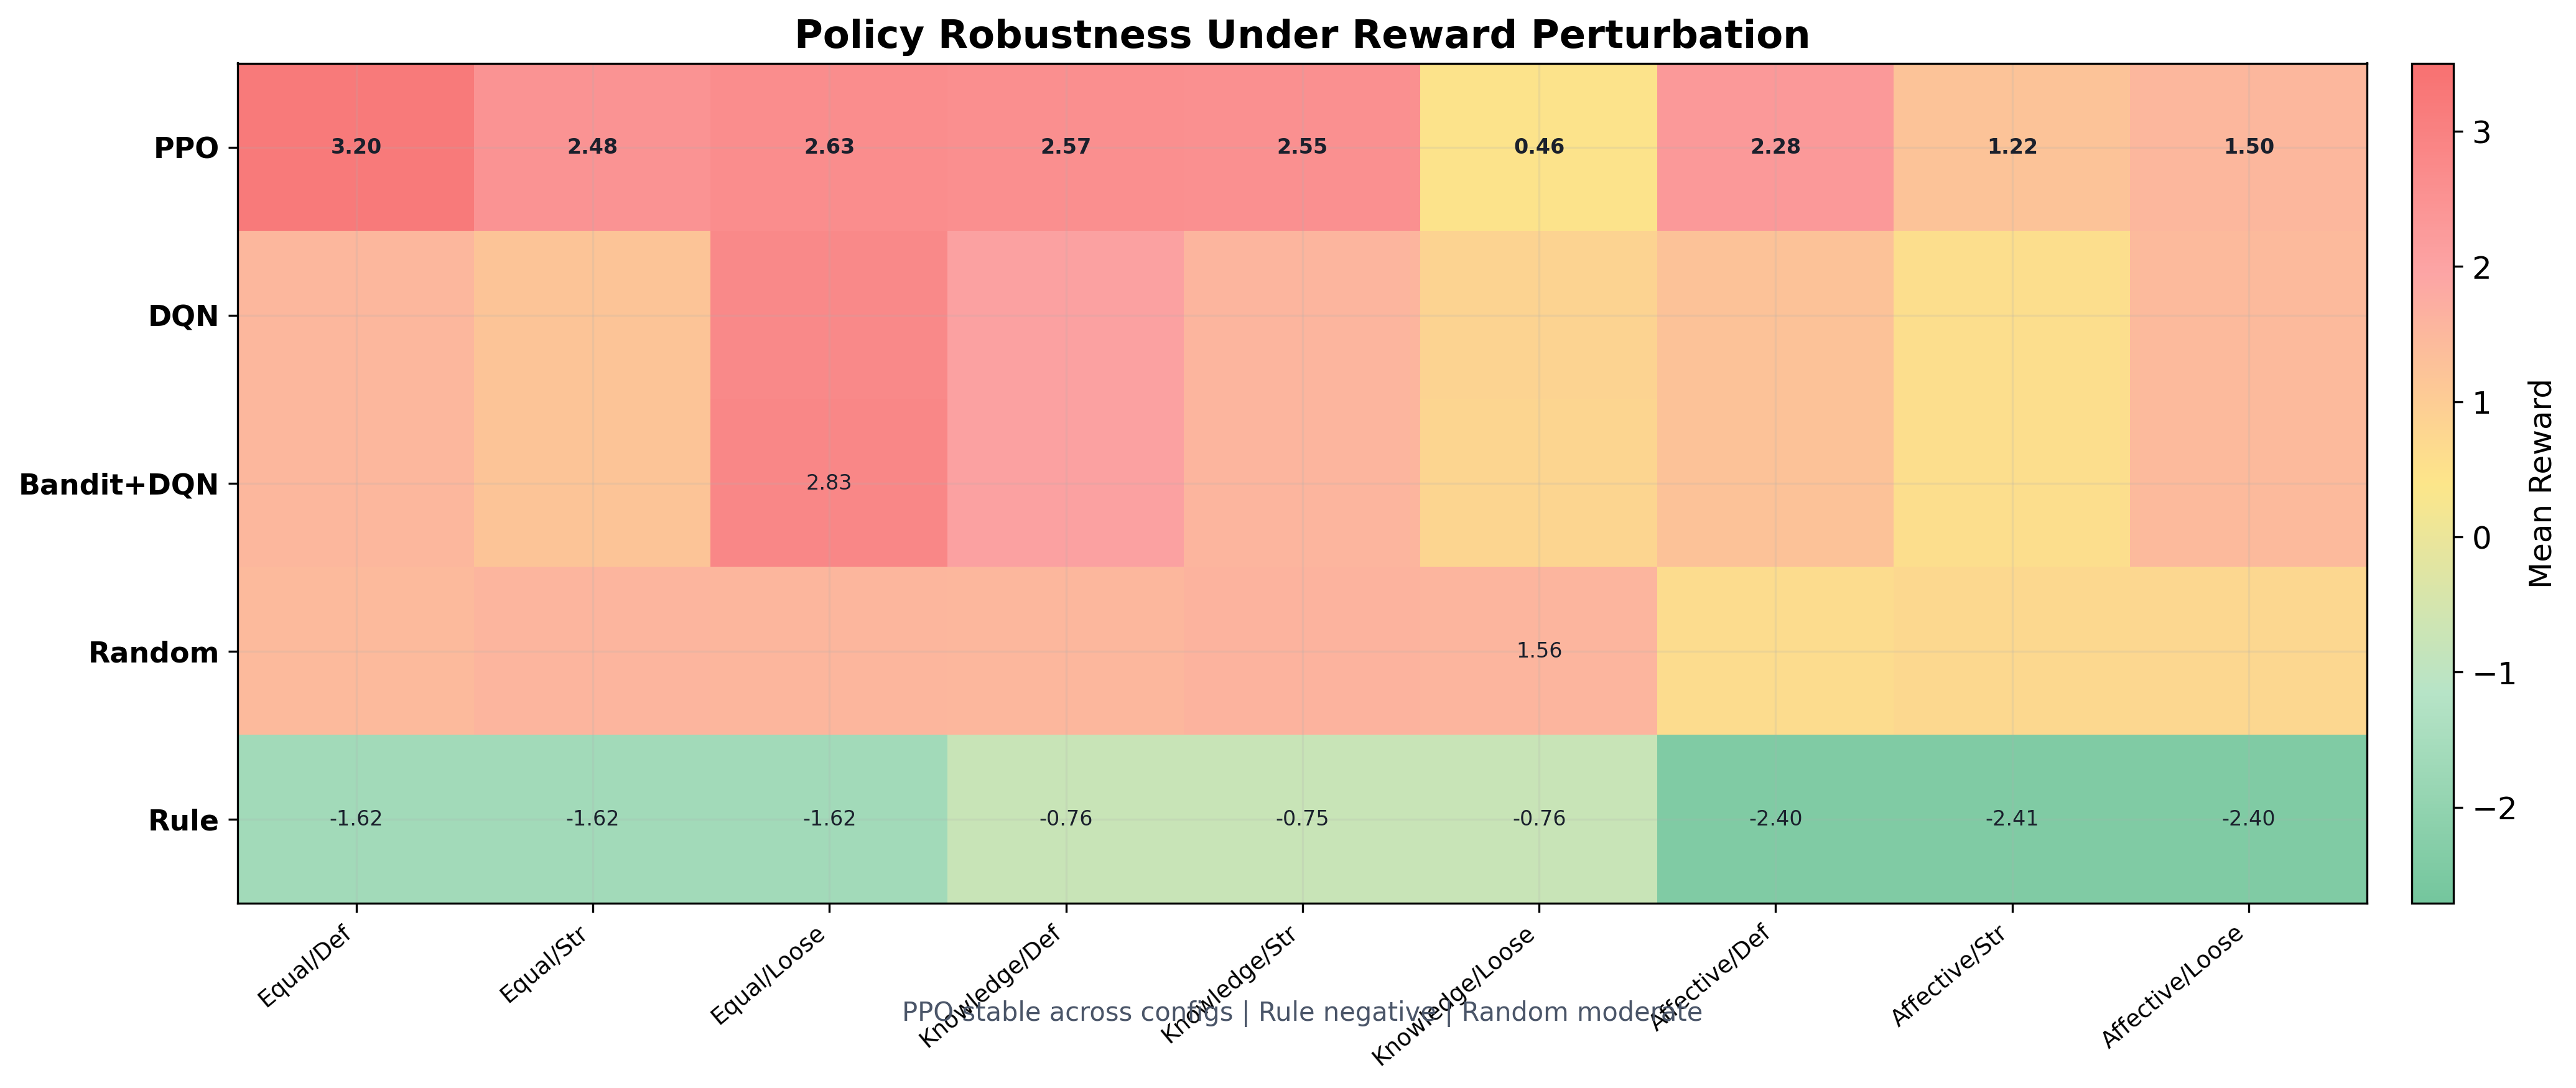
\includegraphics[width=0.95\textwidth]{Figures/reward_sensitivity_heatmap.png}
    \caption{Reward sensitivity heatmap (factorial design, short training budget). Cell values are mean episode reward; colour indicates magnitude. Used to assess whether algorithm rankings are stable under reasonable hyperparameter shifts.}
    \label{fig:rl_sensitivity_heatmap}
\end{figure}

Spearman rank correlations between algorithm orderings across cells [TODO: insert $\rho$ values from \texttt{sensitivity\_factorial.csv} or Figure~\texttt{fig4\_spearman.png}] indicate whether PPO remains top-ranked when weights or masks change. \textbf{Low-budget sensitivity is indicative, not definitive}: $5$k steps are insufficient for full convergence, and single-seed factorial runs ignore cross-seed variance. The analysis supports \emph{directional} robustness checks only, as stated in Section~\ref{sec:method_sensitivity}.

If PPO remains first in most cells, deployment engineers gain confidence that the choice of PPO is not an artifact of a single weight vector. Large rank swaps would flag that reported conclusions are hyperparameter-contingent.

\subsection{Student-Type Breakdown}\label{sec:results_adapt_student_types}

Synthetic students are tagged post hoc as \texttt{fast\_learner}, \texttt{slow\_learner}, \texttt{easily\_frustrated}, or \texttt{patient} based on personality thresholds (Section~\ref{sec:method_synthetic_student}). Stratified metrics test whether policies personalize or merely average performance.

\begin{table}[H]
\centering
\caption{Mean normalized learning gain by student type (placeholder).}
\label{tab:student_type_breakdown}
\begin{tabular}{lcccc}
\toprule
\textbf{Type} & \textbf{PPO} & \textbf{DQN} & \textbf{Rule} & \textbf{Random} \\
\midrule
Fast learner & [TODO] & [TODO] & [TODO] & [TODO] \\
Slow learner & [TODO] & [TODO] & [TODO] & [TODO] \\
Easily frustrated & [TODO] & [TODO] & [TODO] & [TODO] \\
Disengaged / bored & [TODO] & [TODO] & [TODO] & [TODO] \\
\bottomrule
\end{tabular}
\end{table}

[TODO: generate \texttt{learning\_gain\_by\_type.png} via \texttt{evaluation/plots.py} from episode logs.] Expected patterns if PPO generalizes: competitive gain on \texttt{fast\_learner} without excessive frustration on \texttt{easily\_frustrated}; rule-based high gain on fast learners but elevated dropout on frustrated types. Without populated tables, student-type conclusions remain hypothetical.

\subsection{Failure Cases and Limitations}\label{sec:results_adapt_failures}

Several failure modes appeared consistently during evaluation and log inspection:

\paragraph{Over-scaffolding and support loops.} Rule-based and occasionally PPO policies repeat \texttt{scaffold} and \texttt{hint} while engagement drops, triggering boredom penalties without commensurate knowledge growth.

\paragraph{Reward hacking toward zone bonus.} Policies that temporarily raise engagement and lower affect just enough to enter the flow zone can harvest $+1/7$ bonus without sustained learning; masking mitigates but does not eliminate this.

\paragraph{Repetitive action loops.} Cooldowns limit consecutive hints, yet pacing and motivation can still cycle until timeout.

\paragraph{DQN instability.} High seed variance and train/eval masking mismatch produce unreliable Q-values; some seeds likely underperform random on reward.

\paragraph{Persistent frustration and dropout.} When personality parameter $\rho_s$ is low, even reasonable policies may fail to reduce $f$ before five persistent steps trigger termination---a simulator failure case that should not be blamed solely on RL.

\paragraph{Simulator limits.} No item bank, no multimodal input, Markovian affect on five scalars, and uniform personality sampling restrict ecological validity (expanded in Section~\ref{sec:results_adapt_validity}).

\subsection{Discussion}\label{sec:results_adapt_discussion}

The adaptation experiments support four cautious conclusions \textbf{within the synthetic tutoring environment}:

\begin{enumerate}
    \item \textbf{PPO with action masking} is the most reliable learner for maximizing mean shaped reward under equal weights, with reproducible seed behavior ($3.596 \pm 0.112$).
    \item \textbf{Value-based baselines (DQN, Bandit+DQN)} underperform primarily on reward and stability, not necessarily on raw learning gain, highlighting metric trade-offs and implementation asymmetries (masking, network size, sample budget).
    \item \textbf{Hand-crafted rules} optimize knowledge gain but violate the joint reward, demonstrating that expert narratives alone do not substitute for policy optimization under explicit affective costs.
    \item \textbf{Discrete \texttt{emotion\_id}} supplies measurable benefit for reward and rule-consistency, but is partially redundant with continuous affect; ablation shows higher learning gain when the label is removed, so emotion is neither a panacea nor spurious.
\end{enumerate}

RL is suitable here as a \emph{method for integrating multi-objective tutoring signals} under constraints, not as proof of superior human teaching. The FER module remains architecturally connected but empirically decoupled in main runs: closing the loop requires live experiments with latency, noise, and privacy controls.

\subsection{Practical Implications}\label{sec:results_adapt_practical}

Deployment would face barriers beyond simulator scores: FER latency and misclassification would perturb \texttt{emotion\_id}; webcam use raises privacy and consent requirements \cite{fernandez-herrero_evaluating_2024,vistorte_integrating_2024}; teachers must retain oversight because RL policies optimize a engineered reward, not curriculum standards; and safety-critical masking would need auditing on real classrooms. Positive simulator reward suggests feasibility of \emph{offline} policy iteration, not readiness for unsupervised control of learners.

\subsection{Threats to Validity}\label{sec:results_adapt_validity}

\begin{itemize}
    \item \textbf{Construct validity}: Mean reward reflects researcher-defined weights, not learning outcomes; rule-consistency uses an internal map, not educator judgments.
    \item \textbf{Internal validity}: Simulator transitions are hand-written; results are internally consistent but may not reflect human cognition.
    \item \textbf{External validity}: No study with human participants; conclusions do not generalize to classrooms.
    \item \textbf{FER disconnect}: Main RL runs do not inject DAiSEE-trained FER outputs; end-to-end affect-aware tutoring is untested quantitatively.
    \item \textbf{Metric conflict}: High learning gain can coexist with negative reward (rule-based case); reporting a single metric would mislead.
    \item \textbf{Sample budget}: $50$k steps may under-train DQN; sensitivity uses $5$k steps only.
    \item \textbf{In-distribution evaluation}: Policies are evaluated on the same simulator class used for training; no cross-simulator transfer.
    \item \textbf{Emotion ablation interpretability}: Zeroing \texttt{emotion\_id} leaves correlated affect features; observed effects attribute to the discrete channel, not to ``emotion-free'' tutoring.
\end{itemize}

\subsection{Chapter Summary}\label{sec:results_adapt_summary}

Part~II evaluated affect-aware adaptive tutoring policies in a Gymnasium synthetic environment with ten seeds, $50{,}000$ training steps, and $1{,}000$ evaluation episodes per seed. MaskablePPO achieved the highest mean episode reward ($3.596 \pm 0.112$) and rule-consistency ($0.315$), with low cross-seed variance. DQN and Bandit+DQN lagged on reward ($\approx 1.75$) and stability ($\sigma \approx 0.85$). A rule-based expert achieved the highest normalized learning gain ($0.881$) but negative mean reward ($-1.532$), exposing a sharp trade-off between knowledge-focused heuristics and the multi-objective reward. Emotion-aware PPO outperformed an ablated variant without \texttt{emotion\_id} on reward ($+13.2\%$) and rule-consistency ($+9.8\%$), while the ablated variant showed higher learning gain in the dedicated ablation export---underscoring partial redundancy between discrete and continuous affect. All findings are conditional on \texttt{USE\_REAL\_FER=False} and require human studies, live FER integration, and reward validation before educational claims can be made.

\begin{figure}[H]
    \centering
    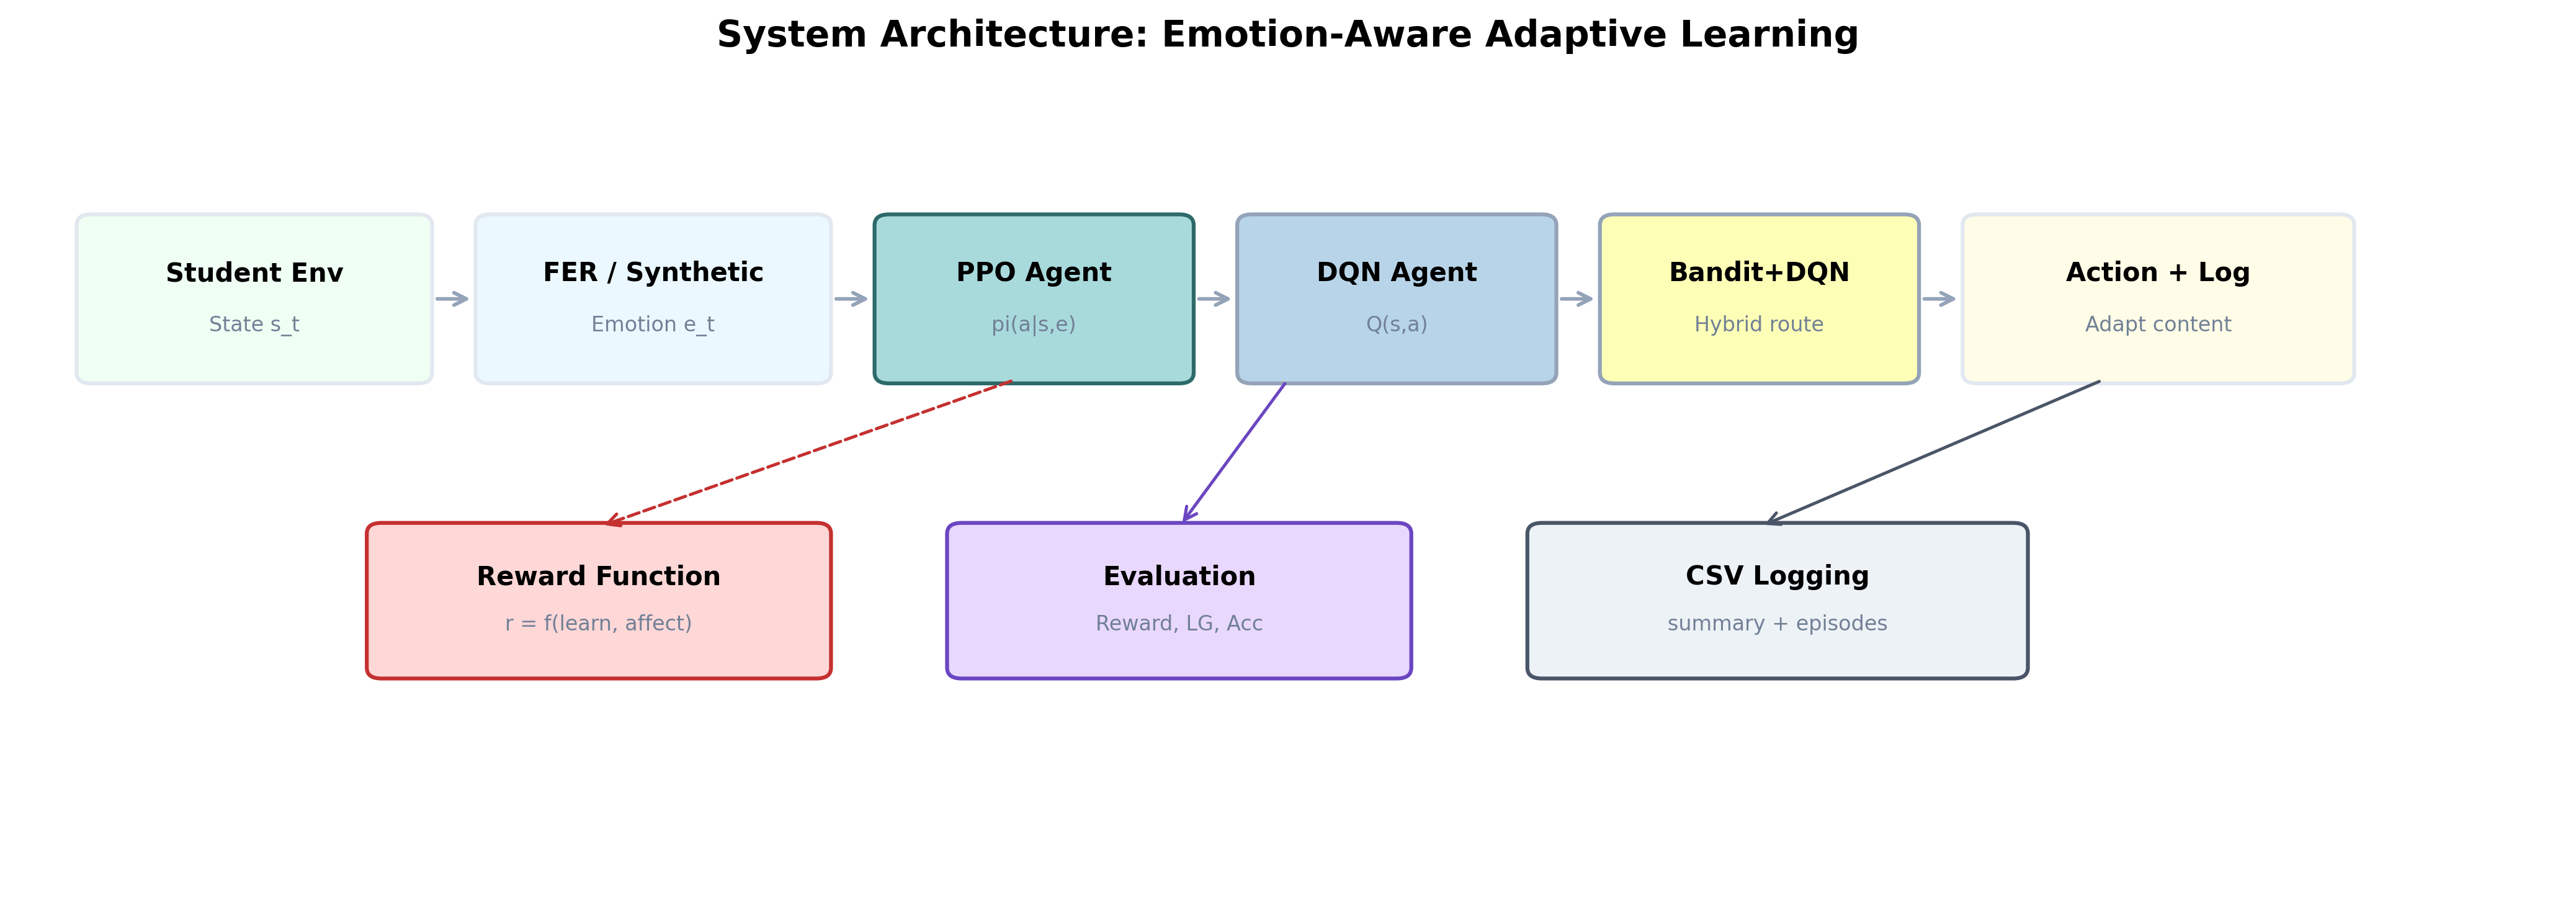
\includegraphics[width=0.95\textwidth]{Figures/architecture.png}
    \caption{Adaptation-module architecture (evaluation pipeline). FER path is optional; thesis experiments use synthetic emotion unless \texttt{USE\_REAL\_FER} is enabled.}
    \label{fig:rl_architecture_results}
\end{figure}

\begin{figure}[H]
    \centering
    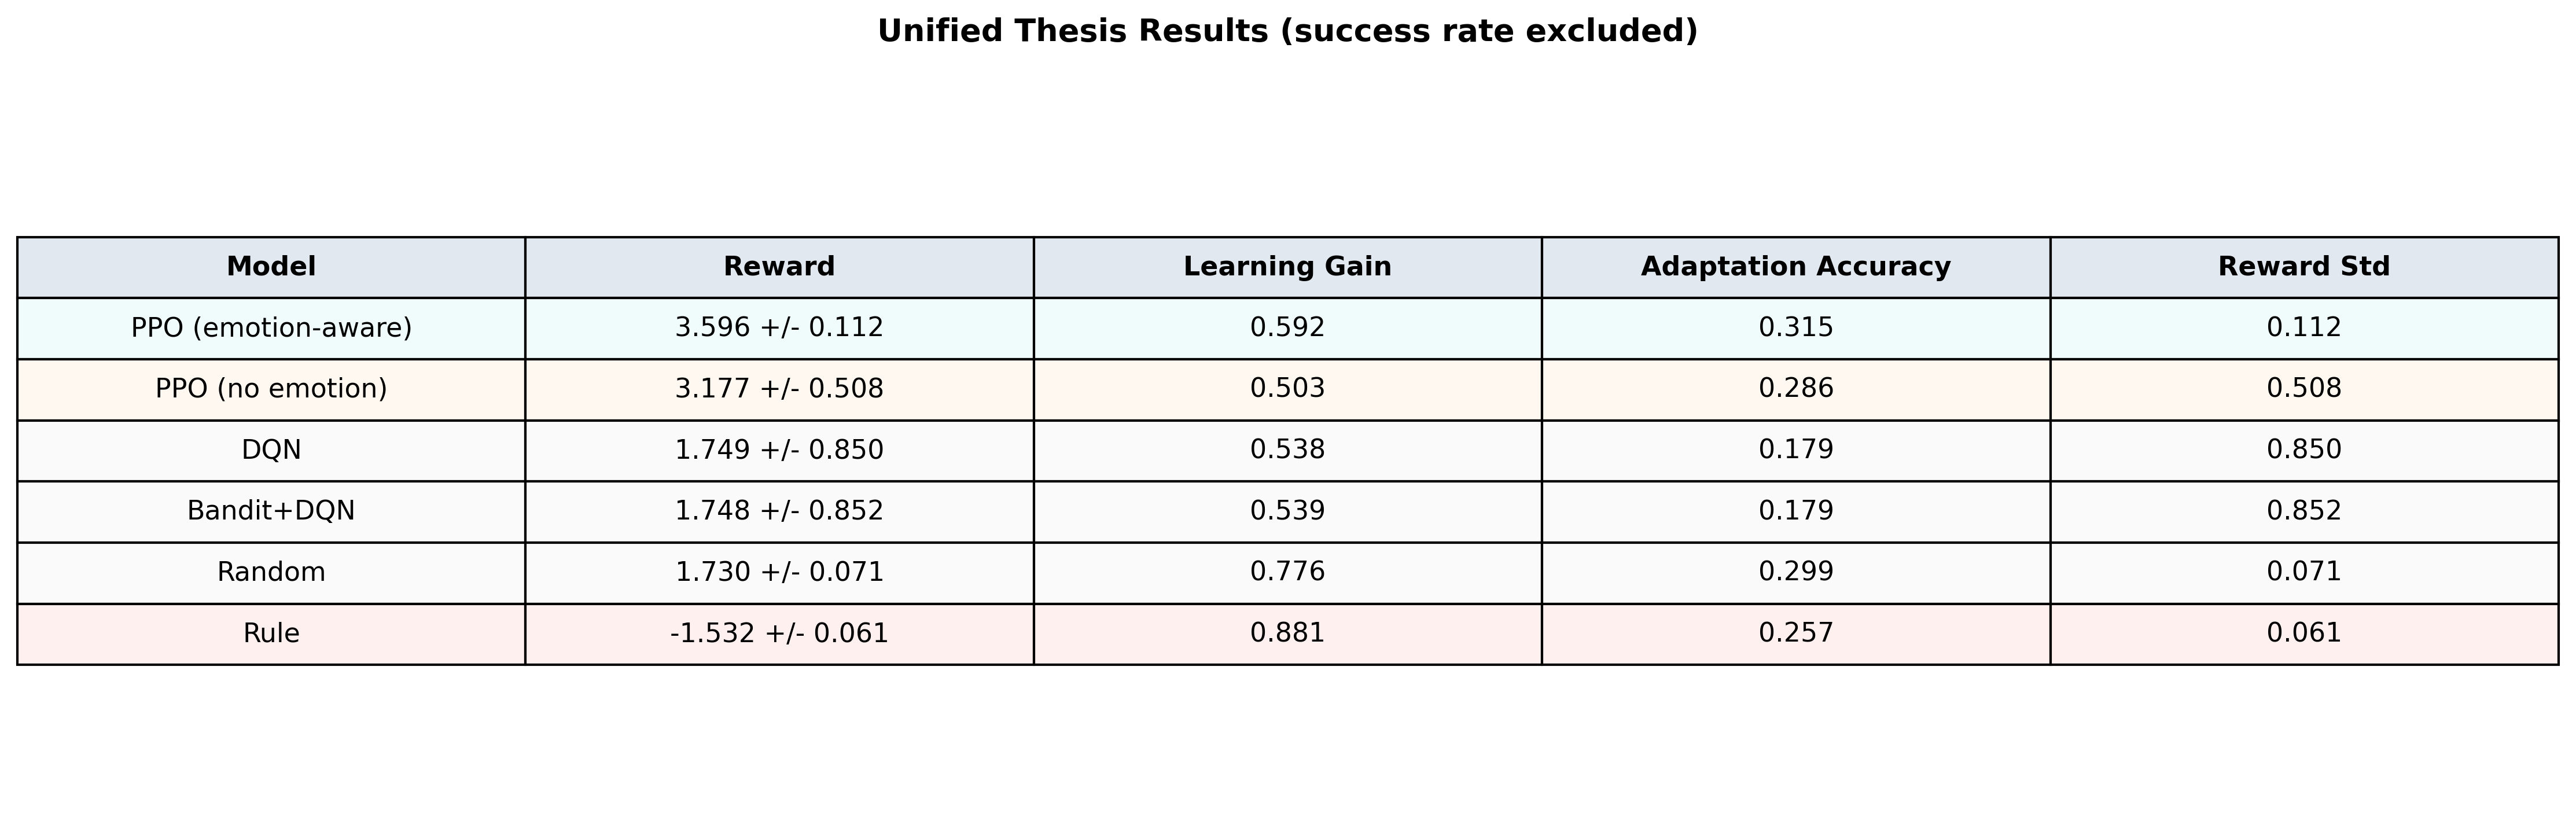
\includegraphics[width=0.95\textwidth]{Figures/final_summary_table.png}
    \caption{Unified summary visualization exported from \texttt{generate\_thesis\_suite.py} (success rate excluded by export design).}
    \label{fig:rl_summary_viz}
\end{figure}
